\documentclass[11pt,twocolumn]{article}
\usepackage{placeins}
\usepackage{fontspec}
\usepackage[margin=0.85in]{geometry}
\usepackage{amsmath,amssymb,amsthm}
\usepackage{booktabs}
\usepackage{graphicx}
\usepackage[authoryear,round]{natbib}
\usepackage{microtype}

\theoremstyle{plain}
\newtheorem{hypothesis}{Hypothesis}
\newtheorem{claim}{Claim}

\title{The DOCAS Framework: A Computational Model of Trust Dynamics as a Parallel Multi-Timescale Neuromodulatory Architecture}
\author{Devon Shigaki~(ORCID: 0009-0003-8977-8010)\\
\small The FreshCredit Lab --- Independent Research\\
\small Correspondence: freshcredit.xyz}
\date{}

% --- Float-page layout tuning: reduce white bands on float-dense pages ---
\renewcommand{\topfraction}{0.85}
\renewcommand{\bottomfraction}{0.70}
\renewcommand{\textfraction}{0.10}
\renewcommand{\floatpagefraction}{0.60}
\renewcommand{\dbltopfraction}{0.80}
\renewcommand{\dblfloatpagefraction}{0.55}
\setcounter{topnumber}{3}
\setcounter{bottomnumber}{2}
\setcounter{totalnumber}{5}
\raggedbottom


\begin{document}

\twocolumn[{%
\maketitle
\begin{abstract}
The companion theory preprint defines trust as the measurable relation between expectation (E) and validation (V), governed by the stability law $\Delta S_t = \lambda(V_t - E_t) = \lambda\varepsilon_t$, with the stack-wide convention $\varepsilon_t = V_t - E_t$ (validation-minus-expectation; positive $\varepsilon$ is a confirmation). This paper specifies the theory's biological instantiation. Because the five neuromodulatory systems involved operate on timescales spanning more than four orders of magnitude (0.1 s to $\sim$2,700 s; up to five if serotonergic tone is included) — phasic dopamine bursts of $\sim$100–400 ms versus the cortisol awakening response peaking 30–45 minutes after awakening — no serial five-step cascade is physiologically coherent. DOCAS is therefore framed here as a \textbf{parallel, multi-timescale modulation architecture}: five neuromodulatory channels — Dopamine, Oxytocin, Cortisol, Adrenergic/noradrenergic arousal, Serotonin — each carrying, predominantly, one of five computational functions that together constitute one trust measurement: Expectation, Validation, Recognition, Activation, Stabilization. The word ``stage\'\' is retained as the name of a \textit{functional role}, not a serial step; the five channels run concurrently and interact through a closed loop in which the stabilized model becomes the next expectation. Each channel is defined functionally, with explicit justification against common mislabelings (dopamine $\neq$ ``reward\'\'; oxytocin $\neq$ ``trust molecule\'\' or ``bonding hormone\'\'; cortisol $\neq$ generic ``stress\'\'; serotonin $\neq$ ``status/contentment\'\'). We formalize channel interactions through $\tau$ = -EFE, the negative of expected free energy as introduced in active inference \citep{friston2015,friston2017}, with valence $= \mathrm{sign}(\Delta\tau)$, arousal $= |\Delta\tau|$, dominance $= d(\Delta\tau)/dt$, situating the architecture within predictive-processing and constructed-emotion theory — engaging the latter where it agrees with DOCAS (anti-essentialism) and where it departs (a functional carrier mapping as a working coordinate system). A genetics section evaluates loci by modern evidentiary standards — genome-wide significance \textbf{and} independent replication. Under that two-gate standard, stated plainly: PDE4B does \textbf{not} pass. Its lead variant rs7528604 reached genome-wide significance for anxiety and stress-related disorders in the iPSYCH case-cohort ($p = 5.39 \times 10^{-11}$, OR = 0.89; \citealp{meier2019}) but failed its lookup in the largest independent anxiety GWAS ($p = .18$, OR = 0.97; \citealp{purves2020}). The PDE4B $\to$ cAMP $\to$ trust-sensitivity-$\lambda$ mechanism is therefore presented as a labeled hypothesis, not a supported mechanism. Historical candidate genes (OXTR, AVPR1A, DRD4, COMT, SLC6A4) are reviewed and set aside per the post-2019 replication consensus. A fully specified experimental protocol, pre-registered on OSF prior to data collection — freezing the channel mapping before data collection — is specified as the stack's decisive test of pipeline decodability and channel-signature separability (the carrier mapping itself is gated by pharmacological/PET-level perturbation, which the protocol's wearable streams cannot deliver). All in-silico evidence reported here is instrument-level: no neurochemistry was measured anywhere in this paper.
\end{abstract}
\medskip
\noindent\textbf{Keywords:} dopamine; oxytocin; cortisol; locus coeruleus–norepinephrine; serotonin; predictive processing; expected free energy; PDE4B; candidate-gene replication; pre-registration; neuromodulatory timescales
\par\medskip
{\footnotesize \textit{Epistemic labels used in this paper:} \textbf{[DERIVED]} (follows from stated assumptions), \textbf{[STANDARD]} (textbook results derived for self-containment), \textbf{[ANALOGY]}, \textbf{[HOMOLOGY]}, \textbf{[EMPIRICAL]}, \textbf{[HYPOTHESIS]}, \textbf{[SIMULATION]}.\par}
\bigskip\bigskip
}]
\medskip
\noindent\textbf{Contents}\\[3pt]
{\small\noindent
1. Introduction\\
2. The Five Carriers: Functional Definitions and Justifications\\
3. Formalization: $\tau$ and the Affective Readout\\
4. Genetic Architecture of Trust-Sensitivity\\
5. The DOCAS Experiment (Pre-registered Design)\\
6. Discussion\\
7. Conclusion\\
}
\medskip



\FloatBarrier
\section{Introduction}

The companion theory preprint provides the formal object — the trust vector T = [D, O, C, A, S] and its stability law — but is silent about how a biological observer computes it. That silence is by design: the theory claims scale-invariance, and the biological level is one coordinate system among several. This paper supplies the biological coordinates.

Its central claim, revised under the timescale constraint that forced this revision, is the following. One trust measurement decomposes into five computational functions — expectation, validation, recognition, activation, stabilization — and each function is carried predominantly (not exclusively) by a distinct neuromodulatory system. These five systems do \textbf{not} execute a serial sequence. Their characteristic dynamics span $\sim$100–400 ms (phasic dopamine, phasic locus-coeruleus norepinephrine), seconds (serotonergic patience signals; peripheral sympathetic drive), seconds-to-minutes (oxytocin release tracking social events; tonic LC modes), and tens of minutes (HPA-axis cortisol responses; the cortisol awakening response) — a range of more than four orders of magnitude (0.1 s to $\sim$2,700 s; up to five if serotonergic tone is included) within which a five-step serial cascade completing ``one measurement\'\' in biological real time is physiologically incoherent (see Table 1, \S{}2.8). What the physiology supports is \textbf{parallel, multi-timescale modulation}: five channels acting concurrently on the same expectation–validation loop, each at its own temporal grain, coupled through the loop's closure (the stabilized model becomes the next expectation). The framework is named DOCAS after the five carriers; ``stage\'\' is retained throughout as shorthand for \textit{functional role within the measurement}, never for a serial step.

Three commitments distinguish DOCAS from prior neurochemical accounts of social behavior. First, functional definitions: each system is named for its computational role in the measurement, not for a folk-psychological label. Second, evidentiary discipline: the post-2019 replication crisis in candidate-gene research \citep{border2019} is treated as binding; genetic claims are restricted to findings that pass a two-gate standard (genome-wide significance \textbf{and} independent replication), everything else is labeled hypothesis — and this paper applies that standard to its own lead candidate, which fails the replication gate (\S{}4.2). Third, testability: the channel mapping is frozen by pre-registration before data analysis, making the framework falsifiable in a way that post-hoc neurochemical narratives are not.

\subsection{Hypotheses and proof obligations}

\begin{hypothesis}[Null hypothesis, H0]
Emotions are innate, hardwired categories, and the five neurochemical systems are independent scalars: no cross-channel coordination, no correlation between the architecture's representational geometry and cortical or cross-linguistic geometry, and no near-critical cortical dynamics. The conjunction is stated with its evidential bookkeeping made explicit: the first conjunct (innate hardwired categories) is already rejected by the field consensus this paper itself cites (\citealp{lindquist2012}; Barrett's constructed-emotion program), so it carries no discriminative weight in either direction --- the test's weight sits entirely on the distinctive conjuncts: the channel-coherence (cross-channel coordination), geometry-correlation, and near-criticality claims.
\end{hypothesis}

\begin{hypothesis}[Alternative hypothesis, H1]
Emotions are constructed from prediction errors via the five DOCAS functions; the five neuromodulatory systems form a coordinated parallel architecture whose representational geometry \textbf{correlates measurably} (not ``is isometric to\'\') with cortical and cross-linguistic semantic geometry; and cortical dynamics are hypothesized — against an active and unresolved methodological controversy (\S{}4.4) — to operate near criticality. The H1 wording is deliberately matched to the evidence the stack has actually delivered: the delivered cross-geometry correspondence is Mantel r = 0.252 (cortical) and 0.240 (embedding), with a recorded null on out-of-distribution stimuli (\S{}4.6) — correlation, not isometry.
\end{hypothesis}

The framework's proof obligations, mapped to their tests: (1) TRIBE — DOCAS-labeled naturalistic stimuli produce separable predicted cortical patterns (TRIBE, the Algonauts 2025-winning fMRI-prediction model; \citealp{dascoli2025,dascoli2026}, supplies the prediction engine; discharged in silico with the released TRIBE v2 weights in \S{}5.2); (2) Gallant/Huth — predicted cortical vectors align with the semantic atlas of natural speech \citep{huth2016}; (3) CLICS — cross-linguistic colexification distances (CLICS 4.0, 3,000+ languages; \citealp{rzymski2020}) correlate with cortical distances under Mantel test; (4) vec2vec — the geometries are partially translatable through the shared latent space demonstrated by \citet{jha2025}; discharged at instrument level in \S{}5.2 (released translators verified with real transfer; the DOCAS-specific LLaMA $\leftrightarrow$ eng1000 bridge built and validated as a supervised ridge map, so vec2vec GAN training is unnecessary in this paired setting); (5) criticality — avalanche statistics evaluated against the contested critical-brain literature with its negative results included (\citealp{beggs2003}; \citealp{touboul2010,touboul2017}; \citealp{destexhe2021}; \citealp{srinivasan2024}; \S{}4.4); (6) PDE4B — now a \textbf{hypothesis} that cAMP gain control contributes to individual differences in the trust-sensitivity coefficient $\lambda$, the discovery association having failed independent replication (\S{}4.2); (7) cooperation — the social coupling term is validated by the evolutionary-game-theoretic record \citep{axelrod1984,imhof2007}.

Obligations 1–4 constitute a single empirical claim: that cortical, semantic, and linguistic geometries share measurable mutual information — that their pairwise distance matrices correlate beyond chance under Mantel test with frozen stimuli and frozen thresholds. That is the ``trust is the basis of meaning\'\' thesis stated so it can fail — and, on current evidence, it is partially supported at effect sizes far below any isometry claim (\S{}4.6, \S{}5.2), with two pre-registered nulls (Sim D8 multilingual arms; Sim D9 second encoder) and one forked result (Sim D11 null $\to$ Sim D13 marginal positive) recorded as such.


\FloatBarrier
\section{The Five Carriers: Functional Definitions and Justifications}

\subsection{D — Dopamine as Expectation}

Dopamine carries the Expectation function: phasic dopaminergic signaling encodes reward prediction errors — the signed difference between anticipated and received outcomes \citep{schultz1997}. ``Expectation\'\' is preferred to ``reward\'\' because the dopaminergic signal tracks the predictive model itself, not hedonic value: momentary subjective well-being is explained by the recent history of expectations and prediction errors, with model weights significant at Z > 3.3, p < 0.001 \citep{rutledge2014}, and pharmacological dopamine manipulation causally shifts even abstract, non-survival rewards such as music \citep{ferreri2019}. In the trust architecture, dopamine carries E — the precision-weighted anticipation of the counterparty's behavior.

Two qualifications from the dopamine literature itself. First, the phasic signal is temporally fine: RPE bursts have $\sim$100–300 ms latency and $\sim$100–400 ms duration \citep{schultz1998}, and sub-second striatal dopamine transients are confirmed in humans \citep{kishida2011} — while tonic dopamine (minutes) does different work (motivation, vigor). ``Expectation\'\' therefore names the fast phasic channel of the D system, not the whole of dopaminergic function. Second, the phasic response is itself composite: \citet{schultz2016} now frames it as an initial unselective salience/detection component followed by a value-coded RPE component, which undercuts any clean ``expectation-only\'\' label. Dopamine also encodes salience, risk, and novelty. The DOCAS claim is the weaker, defensible one: the \textit{predominant} computational role of phasic midbrain dopamine, under naturalistic conditions, is precision-weighted prediction-error signaling — which is what the Expectation function requires. This update rule family — a leaky delta rule driven by signed prediction error — is isomorphic to Rescorla–Wagner learning \citep{rescorla1972} and constant-step-size temporal-difference learning \citep{sutton2018,daw2014}; the framework's contribution is not the update rule but the coupling of five such error-driven channels into one measurement loop, and its fixed-$\lambda$ simplification is knowingly behind the volatility-adaptive Bayesian learners of \citet{behrens2008} (\S{}6, limitations).

\subsection{O — Oxytocin as Validation}

Oxytocin carries the Validation function: the gating of social feedback that registers whether the environment confirmed the expectation. This requires explicit departure from two legacies, now stated completely.

\textit{Against the ``trust molecule\'\' framing:} the foundational intranasal-oxytocin trust effect \citep{kosfeld2005} is dead. Meta-analysis of the trust-game literature (pooled n = 481) finds a combined effect statistically indistinguishable from zero — d = 0.077, 95\% CI $[-0.124,\ 0.278]$, p = .45 \citep{nave2015} — and a pre-registered, high-powered, double-blind registered replication found no effect \citep{declerck2020}. A mechanistic critique compounds the statistical one: only $\sim$0.005\% of an intranasal dose reaches CSF \citep{leng2016}. \textit{Against the ``bonding hormone\'\' framing:} oxytocin's effects are context- and person-dependent \citep{bartz2011}, amplifying the salience of social cues for good or ill — envy and in-group bias alongside prosociality — the social-salience account \citep{shamay2016}; a related reframing casts oxytocin as an allostatic/flexibility regulator \citep{quintana2020}.

Validation, in DOCAS, is precisely a salience-gated confirmation signal: oxytocinergic modulation determines whether returned feedback is registered as validating, and from whom — the O component of the trust vector. The framework's oxytocin claim therefore does not rest on the failed Kosfeld-line literature; it rests on the salience literature that superseded it. What the relationship literature adds is the validation loop's persistence: oxytocinergic signaling is central to the formation and maintenance of social relationships, and its disruption by the loss of affectionate bonds contributes to emotional disequilibrium and elevated risk for stress-related disorders \citep{hurlemann2016} — the biological cost of a validation channel going silent. The timescale honesty applies here too: endogenous oxytocin release tracks social events over seconds to minutes, and exogenous intranasal effects peak $\sim$30–90 min post-administration \citep{leng2016} — nothing supports oxytocin as a fast, millisecond-scale signal, and DOCAS does not claim one.

\subsection{C — Cortisol as Recognition}

Cortisol carries the Recognition function: the HPA-axis precision signal that flags mismatch between expectation and validation. ``Recognition\'\' is preferred to ``stress\'\' because glucocorticoid release tracks novelty, uncertainty, and salience — the detection of discrepancy — rather than a unitary aversive state \citep{ulrichlai2009}. The empirical signature is specific: meta-analytically, cortisol elevations are elicited by unpredictability, uncontrollability, and social-evaluative threat — precisely the conditions of model mismatch — not by generic demand \citep{dickerson2004}. Elevated glucocorticoids increase vigilance and promote exploratory or corrective action \citep{grupe2013}; successful recognition — restoration of predictability and control — terminates the cortisol response \citep{dickerson2004}; and persistent recognition failure produces chronic stress and allostatic load \citep{mcewen1998}.

The timescale caveat is sharpest here. Cortisol has no fast dynamics: acute-stress cortisol peaks $\sim$20–40 min after stressor onset \citep{dickerson2004}, and the cortisol awakening response — a superimposed 50–60\% rise peaking $\sim$30–45 min after awakening, anticipating the day's demands — is a robust, dissociable diurnal component \citep{fries2009,stalder2016}. Cortisol is therefore a \textbf{slow integrative} recognition signal, not a discrete event detector; in a parallel architecture this is a feature (the C channel integrates mismatch evidence over minutes, feeding the retention dynamics of the S channel) rather than a stage in a second-scale sequence. In the formalism of \S{}2.9, C's output is the recognition gate $r_t \in [0,1]$ — the fraction of the mismatch admitted into the stabilization update — not an event timestamp.

This is the function whose absence distinguishes failed trust strategies: tit-for-tat, which mechanically mirrors without re-estimation, is never selected under noise, while win-stay/lose-shift — the strategy with a functioning recognition step — is selected \citep{imhof2007}.

\subsection{A — Adrenergic/noradrenergic Activation}

Epinephrine is a peripheral adrenal-medulla hormone; norepinephrine is the central neuromodulator released by the locus coeruleus (LC). They are distinct systems, and catecholamines do not cross the blood–brain barrier \citep{kostrzewa2007,tank2015}: circulating epinephrine cannot be the carrier of a central activation signal. Peripheral epinephrine influences brain function only indirectly, via vagal afferents (peripheral $\beta$-receptors $\to$ nucleus tractus solitarius $\to$ LC; \citealp{miyashita2006}).

The A channel is therefore defined as \textbf{central noradrenergic arousal}, with peripheral sympathoadrenal activation as a coupled but distinct somatic channel. The locus-coeruleus–norepinephrine system exhibits the clearest \textit{mode-switching} dynamics of any neuromodulator: phasic LC bursts ($\sim$100–200 ms latency, task-event-locked) support exploitation and focused performance, while tonic LC mode (seconds–minutes) supports disengagement and exploration, with transitions driven by utility assessments in ACC/OFC — the adaptive-gain theory \citep{astonjones2005,berridge2003}. The label A is retained — now read as \textit{adrenergic/noradrenergic arousal} — and the modulator vector of \S{}2.9 carries NA (norepinephrine), not epinephrine, as its fourth component; peripheral epinephrine enters the model only as a vagally relayed somatic input to the LC.

The Activation function converts recognized mismatch into action selection. ``Activation\'\' is preferred to ``arousal\'\' because the channel's repertoire is structured by the organism's model confidence, not by a single reflex: fight/flight reflects high-confidence model mismatch triggering immediate motor output to reduce prediction error via approach or avoidance \citep{cannon1929,fanselow1988}, while freeze is a controlled, adaptive immobility — not passive shutdown — induced when prediction error is high and model confidence is low; it functions as a data-gathering action that suppresses premature output, maximizes sensory intake, and accelerates model updating \citep{blanchard1988,deberker2016}. Activation is the behavioral output channel of the architecture and corresponds to the corrective term that dissipates $\varepsilon$ at rate $\mu$ in the theory's dynamics (companion theory preprint, \S{}3.2).

\subsection{S — Serotonin as Stabilization}

Serotonin carries the Stabilization function: the serotonergic systems implicated in patience and behavioral inhibition implement S — the updated prior that the stabilized interaction leaves behind. The defensible evidence is specific, and the pop-science framing is dropped: ``status\'\' and ``contentment\'\' claims trace to popular accounts, not to any citable mechanism, and are not used here.

The positive evidence: optogenetic activation of dorsal raphe 5-HT neurons extends waiting for delayed reward, modulated by reward probability and timing uncertainty \citep{miyazaki2014,miyazaki2018}; and the behavioral-inhibition tradition argues that 5-HT restrains premature responding \citep{soubrie1986}, with prefrontal 5-HT depletion causing reversal-learning inflexibility \citep{clarke2004} and acute tryptophan depletion increasing punishment-driven rejection of unfair offers \citep{crockett2008}. The contrary evidence, which must be cited with it: \citet{fonseca2015} showed DRN 5-HT activation promotes waiting \textbf{but is not reinforcing} — directly contradicting any ``stabilization-as-reward/contentment\'\' reading; serotonin reduces harm-aversion costs in moral decision-making rather than simply encoding punishment \citep{crockett2015}, undercutting the opponent-aversive-channel account \citep{daw2002}; and newer accounts assign 5-HT to cognitive flexibility rather than stability per se \citep{matias2017}. ``Stabilization\'\' is thus defensible specifically as \textbf{patience/behavioral inhibition} — the retention horizon over which outcomes revise the baseline — and is labeled a working interpretation, not an established one.

Stabilization closes the recursive loop: today's S becomes tomorrow's E, which is why trust dynamics compound — stability begets stability at rate $\lambda$, and instability likewise.

\subsection{Functions, not essences: why this is not a ``one chemical = one emotion\'\' claim}

DOCAS must be distinguished from the essentialist program that affective neuroscience has spent two decades dismantling. The locationist hypothesis — that discrete emotion categories are consistently and specifically localized to dedicated brain circuits — failed meta-analytic test: no emotion category maps to a dedicated locale \citep{lindquist2012}. Network neuroscience converges on the same verdict from a second direction: cognitive and emotional capacities are properties of distributed, overlapping network interactions rather than of dedicated substrates \citep{bassett2017}, and emotion specifically is better modeled as large-scale cortical–subcortical network integration spanning the neuroaxis than as localized circuits \citep{pessoa2017}. The chemical version of that hypothesis (``dopamine = pleasure\'\', ``oxytocin = love\'\', ``cortisol = stress\'\') fails with it, and DOCAS does not revive it. The framework makes three weaker, different claims:

1. 	extbf{Each channel is a function, not a feeling.} The five functions are operations in a measurement process — predict, compare, flag, mobilize, consolidate. A function is defined by what it does to the trust vector, not by any phenomenal quality it supposedly contains. Whether a function ``feels like\'\' anything is outside the framework's scope.
2. \textbf{Each named neuromodulator is the predominant carrier of its function, not its sole or sufficient cause.} Every function is modulated by other systems: validation is dopaminergically gated as well as oxytocinergic; recognition recruits noradrenergic and serotonergic co-modulation; activation is HPA-coupled. ``Predominantly, not exclusively\'\' is a claim about relative contribution under naturalistic conditions — falsifiable by measuring the minority contributions — not a claim of molecular exclusivity.
3. \textbf{The carrier-to-function mapping is a working coordinate system, justified by explanatory yield, not by anatomical identity.} The same humility applies that the framework demands of its critics: the mapping stands or falls on whether separable channel signatures are found --- and the pre-registered protocol (Section 5) tests only pipeline decodability and separable channel signatures, \textbf{not} the carrier mapping itself: HRV, sleep, and activity measures are several inference steps from neuromodulatory tone and cannot distinguish the named carriers; pharmacological or PET-level perturbation is the actual gate for carrier claims --- not on whether any chemical is ``really\'\' expectation. (The relationship of this claim to constructed-emotion theory — which licenses the anti-essentialism and predicts degeneracy against it — is engaged directly in \S{}3.)

\subsection{The regulatory parallel: minority activation is the rule at the genetic level too}

The predominant-carrier claim has a precise analog in the framework's own genetics. Section 4 sets aside the historical candidate genes (OXTR, AVPR1A, DRD4, COMT, SLC6A4) not because those loci are inert but because they fail the genome-wide significance gate as primary determinants — they remain plausible minority modulators with small, context-dependent, or interaction effects below the detection threshold of current GWAS power \citep[major depression; the trust-relevant candidate literature shares the same methodology and era]{border2019}. The structure is the same at both levels of the stack: one predominant carrier per function, many minority contributors. And the same discipline applies symmetrically: PDE4B, the framework's lead genetic candidate, passes the discovery gate but \textbf{fails the replication gate} (\S{}4.2), and is accordingly demoted from ``best-supported mechanism\'\' to labeled hypothesis — the two-gate standard (\S{}4.1) is a current-evidence filter, revisable as power increases, and it binds this paper first.

\subsection{One measurement, five parallel timescales}

The five channels are not five independent phenomena, and — the correction this revision makes explicit — not five serial steps either. They are five concurrent modulations of a single measurement act on the trust vector, operating at radically different temporal grains. Table 1 states the constraint quantitatively.

\begin{table*}[t]
\centering\small
\caption{Timescales of the five DOCAS systems (sources in \S{}2.1--2.5).}
\label{tab:timescales}
\begin{tabular}{@{}p{0.16\textwidth}p{0.26\textwidth}p{0.28\textwidth}p{0.22\textwidth}@{}}
\toprule
System (channel) & Fast dynamic & Slow dynamic & Key sources \\
\midrule
Dopamine (D) & phasic bursts $\sim$100–400 ms (RPE) & tonic, minutes (motivation/vigor) & \citealp{schultz1998,schultz2016}; \citealp{kishida2011} \\
\addlinespace
Oxytocin (O) & release tracks social events, seconds–minutes & exogenous effects peak 30–90 min & \citealp{leng2016} \\
\addlinespace
Cortisol (C) & none — no fast dynamics & acute stress peak 20–40 min; CAR peaks 30–45 min post-awakening & \citealp{dickerson2004}; \citealp{fries2009}; \citealp{stalder2016} \\
\addlinespace
LC–norepinephrine (A, central) & phasic bursts $\sim$100–500 ms, event-locked & tonic modes, seconds–minutes & \citealp{astonjones2005}; \citealp{berridge2003} \\
\addlinespace
Peripheral epinephrine (A, somatic) & seconds (sympathetic drive) & minutes; BBB-excluded, vagal afferents only & \citealp{tank2015}; \citealp{kostrzewa2007}; \citealp{miyashita2006} \\
\addlinespace
Serotonin (S) & seconds (waiting promotion) & tonic, hours (mood/flexibility) & \citealp{miyazaki2014}; \citealp{fonseca2015} \\
\addlinespace
\bottomrule
\end{tabular}
\end{table*}

The span — roughly $10^{-1}$ s to $10^{3}$ s — is why a serial five-step sequence is physiologically incoherent and why the architecture is framed as parallel. ``Stage,\'\' wherever the word survives in this paper and its figures, denotes a \textit{functional role in the measurement} (which operation on the trust vector a channel performs), not a temporal step; the channels overlap continuously, and their coupling is given by the loop closure (stabilized S becomes the next E) and by the cross-channel gain structure formalized in \S{}2.9. Figure 1 presents the architecture and its recursive closure. Individual differences in the loop's gain — how violently $\varepsilon$ perturbs S — are parameterized by the theory's trust-sensitivity coefficient $\lambda$; Section 4 evaluates the genetic evidence for its mechanistic substrate, and finds it hypothesis-grade (\S{}4.2).

\subsection{The five functions as mathematical operators}

The functional definitions of \S{}2.1–2.5 can be written exactly. Let $E_{t}$ be the observer's prediction, $V_{t}$ the registered validation, and $\varepsilon_t = V_t - E_t$ the signed mismatch (validation-minus-expectation, so that positive $\varepsilon$ is a confirmation). This is the stack-wide convention; the companion theory preprint now uses the same convention, and the composed law derived below is identical by construction (Technical Appendix, \S{}M4 — the Technical Appendix collects the stack's simulation batteries and mathematical development and is bundled with the Supporting Document (deposit pending); it is cited below as ``Technical Appendix, \S{}M\'\' and ``Technical Appendix, Sim-Battery A/B, Study N\'\'). Each function is one operator on one named channel of the loop:

\begin{itemize}

\item \textbf{D — error-precision gain.} $E_{t+1} = E_t + \alpha_D\,\Pi_t\,\varepsilon_t$, where $\Pi_t > 0$ is the precision (inverse variance) assigned to the error channel. Dopaminergic function is the multiplicative gain on the prediction-error term: the signal scales how much the observed mismatch moves the model (\citealp{schultz1997}; precision-weighting in predictive processing; \citealp{rutledge2014}).
- \textbf{O — social-channel coupling.} $V_t = \gamma_O\,s_t + (1-\gamma_O)\,v_t^{0}$, where $s_{t}$ is the conspecific validation signal, $v_{t}^{{0}}$ the default (unsocial) observation, and $\gamma_O \in [0,1]$ the coupling coefficient. Oxytocinergic function is setting $\gamma_O$ for social sources — the gate that decides which signals count as validation and from whom.
- \textbf{C — mismatch-salience detection.} $C_t = \mathrm{logistic}\!\left(\beta_C\,\left(|\varepsilon_t| - \theta_C\right)\right)$, with $\mathrm{logistic}(\cdot)$ the logistic function. Recognition is a thresholded readout of unsigned mismatch; corticosteroid state translates the threshold $\theta_C$ and slope $\beta_C$. The recognition gate $r_t$ of the master law is a monotone readout of $C_{t}$: the fraction of the mismatch admitted downstream.
- \textbf{A — output gain.} $A_t = g_A \cdot f(\Delta\tau_t)$, $g_{A}$ > 0 scaling the slope that converts recognized mismatch into behavioral output — noradrenergic adaptive gain \citep{astonjones2005} — corresponding to the corrective term that dissipates $\varepsilon$ at rate $\mu$ in the theory's dynamics.
- \textbf{S — integration time-constant.} Serotonergic function is setting the retention horizon $h_{S}$ — the number of steps over which outcomes revise the stabilized baseline — entering the update as the leak $\delta_S = 1/h_S$ (\citealp{shine2021}, map serotonin onto the gain of higher-order belief updating).

\end{itemize}
\textbf{The master update law, DOCAS preset.} The stack's master update law (Technical Appendix, \S{}M4) is

\begin{equation}
\begin{split}
S_{t+1} = {}& S_t + \lambda^{+}\!\cdot\max(\varepsilon_t, 0)\cdot r_t + \lambda^{-}\!\cdot\min(\varepsilon_t, 0)\cdot r_t\\
&- \delta_S\cdot(S_t - S_{\mathrm{base}})
\end{split}
\tag{ML}\label{eq:ml}
\end{equation}

with $\lambda^{+}, \lambda^{-} \geq 0$ the confirmation/betrayal sensitivities, $r_t \in [0,1]$ the recognition gate, $\delta_S \geq 0$ the retention leak, and $S_{base}$ the baseline toward which stabilization decays. The DOCAS biological layer is the preset $\lambda^{+} = \lambda^{-} = \lambda$, $r_t \in [0,1]$, $\delta_S > 0$, \textbf{$S_{base}$ = the homeostatic prior} — the no-information trust state toward which stabilization reverts absent new evidence:

\begin{equation}
S_{t+1} = S_t + \lambda\, r_t\, \varepsilon_t - \delta_S (S_t - S_{\mathrm{base}}).
\tag{DOCAS preset}\label{eq:preset}
\end{equation}

The baseline-restoring form of the leak is not cosmetic. The earlier pure-leak version (decay toward zero) decays trust to zero without events — simulated half-life $\approx$ 69 events at $\delta = 0.01$, exactly matching theory $\ln 2/\delta$ (Technical Appendix, Sim-Battery A, Study 1, fig1a) — which punishes precisely the quiet, thin-file users the stack's cold-start analysis cares about; the baseline-restoring leak avoids the pathology, recovering to within 10\% of $S_{base}$ in 207 events ($-20$ shock; 69/138 for $-5$/$-10$) after a shock-then-silence probe (Technical Appendix, Sim-Battery A, fig1a, fig2). The theory's physics layer is recovered as the \textbf{proven limit} $\delta_S \to 0$, $r \to 1$ of (ML) (Technical Appendix, \S{}M4.2) — the exact statement replacing the earlier, unproven claim that the biological layer ``reduces to the physics layer by construction.\'\' The protocol layer is the further extension $\lambda^{-} > \lambda^{+}$ (break/build asymmetry), an explicitly labeled extension, not part of the DOCAS preset.

Collect the channel gains as $g = (\Pi,\ \gamma_O,\ (\theta_C, \beta_C),\ g_A,\ h_S)$ and the neuromodulatory state as $m = (\mathrm{DA}, \mathrm{OT}, \mathrm{CORT}, \mathrm{NA}, \mathrm{5\mathord{-}HT})$; the modulators act on the loop through a gain matrix $g = M\,m$. The component-wise non-negative vector $a(t) = (\Pi_t, \gamma_{O,t}, C_t, g_A f(\Delta\tau_t), \lambda r_t)$ is what the theory's Fisher–Rao construction normalizes into the stage-mix simplex coordinate $\theta$ (Technical Appendix, \S{}M6.2) — the simplex applies to these non-negative activities, not to the signed components of T.

\begin{claim}[DOCAS, exact form]
M is \textbf{diagonal-dominant} — under naturalistic conditions each modulator's largest-magnitude effect falls on its named channel, $|M_{ii}| > \sum_{j \neq i} |M_{ij}|$ row-wise, and the off-diagonal entries are the framework's named minority activations: measurable, expected nonzero, and the falsification route. If any row's off-diagonal mass exceeds its diagonal entry, that channel assignment is wrong. ``One chemical, one primary function, with minority activations\'\' is thereby a statement about the spectrum of a matrix, not about molecules having single effects.
\end{claim}

Two properties follow immediately and are exercised in \S{}5.3. First, the operators compose into the DOCAS preset of the master law: substituting the D, O, C, and S operators yields (DOCAS preset) above — the stability law with recognition gating and baseline-restoring leak made explicit, whose physics-layer limit is proven, not constructed. Second, because the channels form a closed loop (S feeds tomorrow's E), single-operator lesions propagate along the loop's edges — D reads O's output, S integrates what C passes, and A acts on $\varepsilon$, which is downstream of D — so the framework predicts an \textbf{ordered-cascade lesion signature} rather than five cleanly independent deficits. Whether that cascade signature was a prediction or a post-hoc rationalization is answered in \S{}5.3: as a pre-registered double-dissociation criterion it failed; as post-hoc hypothesis generation it is the next experiment's target.

\begin{figure*}[!tp]
\centering
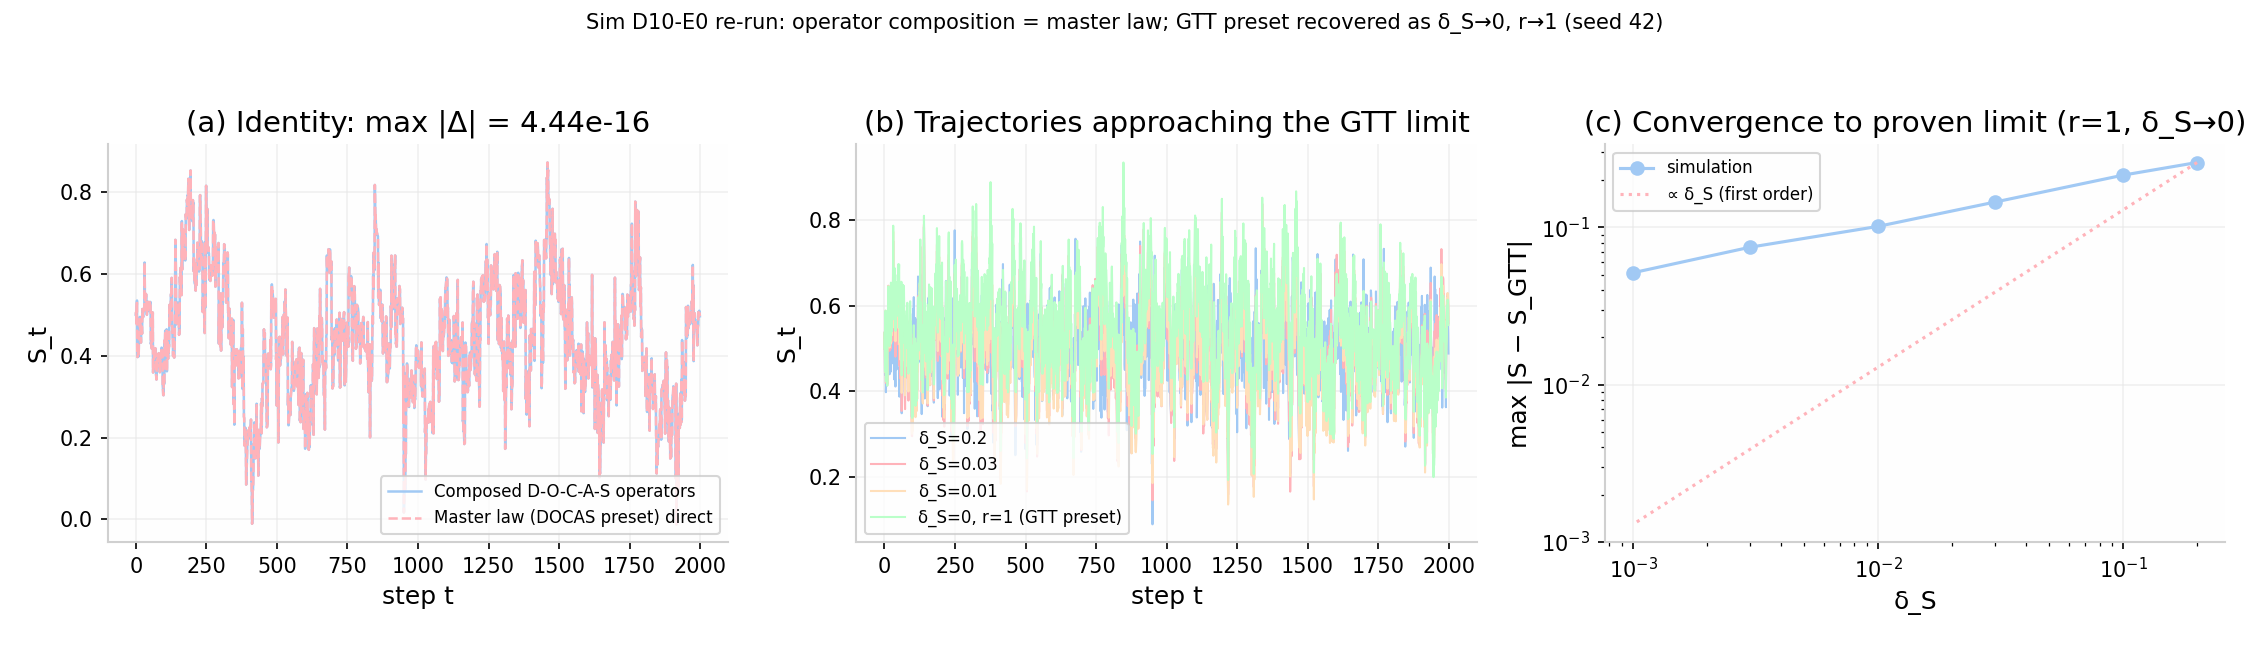
\includegraphics[width=0.92\textwidth]{figures/figD_operators_masterlaw.png}
\caption{Operator composition and master-law verification (independent verification re-run, numpy, seed 42). The composed D$\to$O$\to$C$\to$A$\to$S operator loop reproduces the master-law DOCAS preset to machine precision (max $|\Delta S| = 4.4\times 10^{-16}$ over 2{,}000 steps), and the trajectories approach the theory's physics-layer limit as $\delta_S \to 0$, $r \to 1$. Self-consistency check of the definitions; not evidence about biology.}
\label{fig:operators}
\end{figure*}


\FloatBarrier
\section{Formalization: $\tau$ and the Affective Readout}

Following the free-energy formulation of action and perception, define $\tau$ = -EFE, the \textbf{negative of expected free energy} — precision-weighted confidence that the current policy keeps the organism within expected states. The attribution is explicit: expected free energy, decomposed into epistemic value (information gain) and pragmatic value (expected log-preference), with policies a priori more probable the lower their EFE, is the quantity introduced in active inference by \citet{friston2015} (\textit{Cognitive Neuroscience}) and \citet{friston2017} (\textit{Neural Computation}), building on the free-energy principle \citep{friston2010}. $\tau$ is that quantity with its sign and functional role unchanged; DOCAS's use is an application, not a modification, of the active-inference formalism. Channel interactions in the DOCAS architecture are transitions in $\tau$, and the standard affective dimensions fall out as readouts of its trajectory:

\begin{equation}
\begin{split}
&\mathrm{valence} = \mathrm{sign}(\Delta\tau); \qquad \mathrm{arousal} = |\Delta\tau|;\\
&\mathrm{dominance} = d(\Delta\tau)/dt
\end{split}
\tag{1}\label{eq:readout}
\end{equation}

The three-dimensional readout itself is a re-parameterization of the Pleasure–Arousal–Dominance (PAD) model of \citet{mehrabian1974}, with valence corresponding to pleasure–displeasure; DOCAS adopts the PAD dimensionalization and its established measurement instruments rather than introducing new affective axes.

\textbf{Units and measurability — stated, not waved at.} EFE is a normative computational objective, not a measurable neurochemical signal; no current method measures the expected free energy of a biological policy directly. What equation (1) requires empirically is therefore an estimator chain, and its links differ in quality. $\Delta\tau$ is estimable only through a fitted generative model (behavioral choice data under an active-inference model, with precisions fixed a priori); valence and arousal are directly measurable by PAD self-report and autonomic indices; and the third term is the most fragile: dominance = $d(\Delta\tau)/dt$ is a derivative of a model-estimated quantity, and its value is \textbf{sampling-rate dependent} — the estimated derivative changes magnitude, and can change sign-stability, with the observation cadence, so cross-condition and cross-study comparisons are meaningful only at matched sampling rates and stated estimator settings. What is not measurable at all: the EFE of a policy the organism did not take, and any direct molecular correlate of $\tau$. The framework claims readout structure, not molecular identity.

Emotion, on this account, is the experienced derivative of the trust measurement. Here the relationship to constructed-emotion theory must be stated precisely. Constructed-emotion theory holds that emotions are constructed categories built from interoceptive predictions and learned concepts, with no dedicated biological fingerprint per emotion and with \textbf{degeneracy} — many neural patterns realizing the same emotion category \citep{barrett2017a,barrett2017b,barrett2015}. That theory licenses anti-essentialism; it does not license a fixed five-carrier biochemical mapping, and citing it as support for one is backwards. The statement is in two parts. \textbf{Where DOCAS agrees:} against folk-essentialism — there is no ``fear circuit\'\' or ``trust molecule,\'\' the carrier-to-function mapping is not a claim about essences, and \S{}2.6's three commitments are exactly the anti-essentialist discipline Barrett's program established. \textbf{Where DOCAS departs:} the framework posits a \textit{functional} carrier mapping — predominant, not exclusive, channel assignments (\S{}2.9's diagonal-dominance of M) — as a working coordinate system for measurement. Constructed-emotion theory predicts this mapping should exhibit degeneracy (multiple neuromodulatory realizations of the same functional state); DOCAS's diagonal-dominance claim is therefore in direct, testable tension with full degeneracy, and the pre-registered protocol of Section 5 is precisely where that tension is resolved: if measured stage profiles show many-to-one realizations with no dominant carrier per function, the coordinate system fails and the Barrett-side position wins. Equation (1) retains a lawful affective mapping that pure constructionism under-specifies — while conceding that under-specification may be a feature of the phenomenon, not a gap in the theory.

Equation (1) generates testable correspondences: a confirmed expectation ($V \geq E$) produces $\Delta\tau > 0$ — positive valence with arousal scaled by surprise; a detected mismatch with low coping precision produces negative valence, high arousal, falling dominance — the phenomenal signature of the C channel. Each term of equation (1) is falsifiable separately, and the third is the most exposed: if measured dominance (PAD self-report scales or behavioral control/agency measures) tracks the \textbf{level} of $\tau$ rather than the signed rate of change of $\Delta\tau$, the derivative term is wrong and the readout collapses to two dimensions. The pre-registered signature that keeps the term alive: $\Delta\tau > 0$ with $d(\Delta\tau)/dt$ < 0 must present as positive valence with diminishing agency (the phenomenology of relief subsiding into resignation), and a C-channel mismatch with recovering coping precision must show dominance rising before valence turns. If the empirical order is reversed — valence moving first, dominance following as a lagged consequence — dominance is a downstream readout of valence, not an independent derivative, and equation (1) must be revised.

The framework also yields a principled account of cross-modal trust domains. Music, for instance, is a pure expectation–validation instrument: compositional structure generates predictions whose confirmation or violation drives affect, with dopaminergic transmission causally mediating the reward \citep{ferreri2019,blood2001}. Linguistic communication is another — though the citation must be read in its actual direction: epistemic vigilance \citep{sperber2010} is a theory of \textit{calibrated distrust} — listeners gate comprehension through checks on the source's competence and benevolence, accepting content only insofar as the source passes them. In DOCAS terms, that is the validation function applied to incoming meaning: comprehending a message requires the O channel to admit the source's signal, which is exactly the gate \S{}2.2 formalizes as $\gamma_O$. Recent machine-learning results show that representations of meaning align across independently trained models — vec2vec demonstrates unsupervised translation between language-model embedding spaces via a shared latent structure \citep{jha2025} — consistent with a common geometric substrate on which expectation–validation loops in different modalities could be jointly measured. These cross-modal correspondences are offered as convergent evidence for the measurement framing, not as independent validations of the architecture.


\FloatBarrier
\section{Genetic Architecture of Trust-Sensitivity}

\subsection{Evidentiary standard}

The candidate-gene era produced a literature of small-sample associations between social phenotypes and common variants in OXTR, AVPR1A, DRD4, COMT, and SLC6A4. That literature did not survive genome-wide standards: adequately powered studies find no support for historical candidate-gene hypotheses in behavioral traits \citep[major depression; the trust-relevant candidate literature shares the same methodology and era]{border2019}, and the administration-effects literature is likewise null at meta-analytic scale \citep{nave2015,declerck2020}; the OXTR candidate-gene associations specifically are covered by the post-2019 replication consensus reviewed above. DOCAS therefore adopts a two-gate standard: a locus must show (i) genome-wide significant association with a mechanism-relevant phenotype \textbf{and} (ii) independent replication — with mechanistic plausibility in a trust-relevant pathway required before any mechanism language is used. Both gates are binding on this paper's own candidate.

\subsection{PDE4B and cAMP gain control [EMPIRICAL — two-gate standard NOT met; mechanism claim = HYPOTHESIS]}

Phosphodiesterase 4B hydrolyses cAMP, the second messenger through which dopaminergic, adrenergic, and serotonergic signals are integrated — a molecular gain-control on exactly the pathways that carry the DOCAS functions. The evidence, stated with its failure in the same paragraph as its success: in the Danish iPSYCH2012 case-cohort (12,655 cases, 19,225 controls; register-based diagnoses of combined anxiety \textbf{and} stress-related disorders — not questionnaire anxiety), variants in PDE4B were associated at genome-wide significance: lead SNP rs7528604, $p = 5.39 \times 10^{-11}$, OR = 0.89 (95\% CI 0.86–0.92) — the A allele protective — robust across sensitivity analyses adjusting for psychiatric comorbidity, with SNP-heritability of the phenotype estimated at 28\%, and with a mouse-model arm showing altered Pde4b expression after chronic stress \citep{meier2019}. \textbf{And:} the lead variant failed its lookup in the largest independent anxiety GWAS — UK Biobank, five phenotypes, $\sim$28k–31k cases: rs7528604 $p = .18$, OR = 0.97 (95\% CI 0.93–1.02), attenuated toward null (\citealp{purves2020}; reported by Meier et al. themselves). The framework's own two-gate standard is therefore \textbf{not met}: gate (i) passed, gate (ii) failed. PDE4B is a hypothesis-generating candidate for cAMP-mediated stress/psychiatric vulnerability — not a validated marker of individual differences in stress reactivity, and it licenses no quantitative claims about neuromodulatory channel dynamics. Regulatory-plausibility annotation of the locus adds a mechanistic prior and nothing more: under the pre-registered Sim~D14 gate (criterion frozen before any score was inspected; OSF deposit), AlphaGenome variant-effect scoring \citep{avsec2026} (GRCh38; brain-relevant tracks; the model's common-variant-calibrated quantile scores) places the lead variant and all 23 EUR linkage-disequilibrium proxies ($r^2 \geq 0.8$) in the top-5\% impact band for common SNVs ($|$quantile$| \geq 0.95$; lead $|$quantile$| = 0.9857/0.9852$ for the A/C alleles; band minimum across the set $0.9694$) --- instrument-level, hypothesis-generating evidence that the locus is regulatory-active, which has no bearing on the replication gate above. The measured-tissue leg then fails: in GTEx v8 adult brain \citep{gtex2020,kerimov2023} (all 13 regions; official significant-pair lists plus full summary statistics; pre-registered Sim~D15, criterion frozen before data access; OSF deposit), no variant in the frozen locus set is a significant cis-eQTL or cis-sQTL for PDE4B --- indeed PDE4B has no significant brain eQTL/sQTL pairs at all --- and the strongest nominal association is $p = 1.8 \times 10^{-3}$ (rs11208779, frontal cortex BA9; lead rs7528604 $p = .025$--$.049$), so the Sim~D14 band placement is annotation-only and the hypothesis is downgraded a further notch.

The remaining evidence, with its contradictions intact:

\begin{itemize}

\item \textbf{Mechanism.} PDE4B binds DISC1, an independently identified risk factor for major mental illness; DISC1 sequesters PDE4B at rest and releases it under elevated cAMP/PKA to terminate cAMP signaling, with PDE4B itself disrupted by a familial t(1;16) translocation segregating with psychiatric illness \citep{millar2005}; the cAMP-dependent dissociation differs across DISC1 isoforms and PDE4 subfamilies, an isoform-selectivity caveat (\citealp{murdoch2007}; review: \citealp{millar2007}).
- \textbf{Expression — and the direction contradiction, flagged not resolved.} PDE4B polymorphisms and \textbf{decreased} PDE4B expression are associated with schizophrenia in postmortem brain \citep{fatemi2008}, corroborated by a systematic meta-analysis of ten brain datasets (437 samples), validated in the CommonMind consortium (515 samples) — with the important caveat that the downregulation signal concentrates in a patient subgroup, and that blood and iPSC-derived neuron signals run in the \textit{opposite} direction \citep{burrack2024}. Association studies in schizophrenia are inconsistent in direction and replication across populations. This collides head-on with the framework's model arrow (\S{}4.4): the model maps PDE4B $\downarrow$ $\to$ cAMP $\uparrow$ $\to$ higher effective learning rate / nearer-critical dynamics $\to$ the flexible-updating, high-trust side — yet schizophrenia, a phenotype characterized by paranoia and low social trust, shows PDE4B \textit{downregulation}. The arrow, as stated, points the wrong way for that phenotype. The contradiction is explicitly unresolved: candidate explanations (subgroup concentration of the expression signal; opposite-direction peripheral signals; developmental vs. adult regulation; the anxiety-discovery allele being protective, i.e. \textit{raising} effective PDE4B function) are conjectures, and none is adopted. The $\mathrm{PDE4B} \to \lambda$ mechanism survives only as the labeled hypothesis below.
- \textbf{Functional role in learning.} As the cAMP-degrading enzyme, PDE4B sets the gain on experience-dependent plasticity: reduced PDE4B activity prolongs cAMP signaling, effectively raising the learning rate — a molecular candidate for the theory's trust-sensitivity coefficient $\lambda$. Pharmacologically, PDE4B inhibition shows antidepressant and anxiolytic profiles in animal models.

\end{itemize}
\begin{hypothesis}
Common regulatory variation at PDE4B (including the rs7528604 locus) modulates $\lambda$, the rate at which expectation–validation mismatch revises stabilization. This is a hypothesis, not a supported mechanism: the discovery association did not replicate in the largest independent anxiety GWAS, and the schizophrenia expression data run counter to the model's predicted direction. The specific eQTL effect size and the ancestry-stratified allele-frequency structure of this locus are treated as quantities to be estimated in the pre-registered study (Section 5), not as established values; constraint metrics for the gene will be reported from gnomAD v4 at analysis time. The verified GWAS statistics above are the entire genetic claim; no population-genetic simulation is offered as evidence.
\end{hypothesis}

\subsection{Historical candidate genes: reviewed and set aside [EMPIRICAL — gates failed]}

\begin{table*}[t]
\centering\footnotesize
\caption{Historical candidate genes, and the framework's own lead candidate, under the two-gate standard of \S{}4.1.}
\label{tab:genes}
\begin{tabular}{@{}p{0.07\textwidth}p{0.34\textwidth}p{0.34\textwidth}p{0.17\textwidth}@{}}
\toprule
Gene & GWAS support & Status per post-2019 consensus & Prior claim \\
\midrule
PDE4B & GWS in discovery cohort ($p = 5.39 \times 10^{-11}$; \citealp{meier2019}); \textbf{failed replication} in the largest anxiety GWAS ($p = .18$; \citealp{purves2020}) & Hypothesis-generating only; two-gate standard not met & cAMP gain-control on the architecture \\
\addlinespace
OXTR & No GWS & Small-n, mixed replication; administration-effects meta-analytic null \citep{nave2015}; registered administration replication null \citep{declerck2020} & ``trust/bonding locus\'\' \\
\addlinespace
AVPR1A & No GWS & Repeat-based associations; low variance explained & bonding locus \\
\addlinespace
DRD4 & No GWS & Fails replication & novelty-seeking locus \\
\addlinespace
COMT & No GWS & ``Warrior/worrier\'\' framing debunked at scale & cognitive-stress locus \\
\addlinespace
SLC6A4 & No GWS & G $\times$ E claims heavily qualified & mood/stress locus \\
\addlinespace
\bottomrule
\end{tabular}
\end{table*}

This table is retained deliberately: stating plainly why the famous loci are excluded — and why the framework's own lead candidate is demoted — is part of the framework's falsifiability. Trust-sensitivity is treated as polygenic, with twin-based heritability of mechanism-relevant traits (dopaminergic function, HPA regulation, serotonergic stabilization) moderate but distributed across many loci — consistent with the meta-analytic finding that behavioral trust is only 7–17\% heritable while stated trust is $\sim$33\% \citep{kettlewell2024}.

\subsection{Criticality: a contested operating-point hypothesis [ANALOGY; contested empirical status]}

This section carries a hypothesis of the framework, stated against its own negative literature — not an ornament, and not an established grounding. The founding evidence: cortical networks exhibit avalanche statistics consistent with operation near a critical point — a branching parameter $\nu \approx 1$ , at which each active neuron activates one successor on average \citep{beggs2003} — and dynamic range, information capacity, and information transmission are reported as maximized near that point in model and in-vitro work \citep{kinouchi2006,shew2009,shew2011}. The two sides of the critical point map onto two failure modes of trust. Sub-critical dynamics ($\nu < 1$): activity dies out, prediction error cannot propagate, expectation is frozen regardless of validation — the rigid state produced by chronic C-channel allostatic load, in which E never updates toward V. Super-critical dynamics ($\nu > 1$): activity explodes, noise swamps validation, no expectation survives long enough to be validated — the A-channel runaway state. Convergence $E \to V$ is dynamically realizable, on this hypothesis, only between these regimes.

The contested status must now be stated as plainly as the hypothesis, because the demolitions are substantial and come from both outside and inside the criticality camp. (i) 1/f spectral scaling arises from filtered Poisson processes without any critical state \citep{bedard2006}. (ii) Avalanche power laws arise from random-walk-through-threshold dynamics without criticality \citep{touboul2010}. (iii) Power-law phase-locking intervals arise from thresholding finite data, in empty-room MEG recordings as well \citep{botcharova2012}. (iv) Even the strongest classical signatures — exponent relations plus universal shape collapse — are reproduced by uncoupled neurons driven by correlated noise, and the standard E/I network model shows no information-capacity peak at its transition \citep{touboul2017}; the programmatic conclusion that existing evidence is insufficient is stated in \citet{destexhe2021}. (v) Subsampling alone can manufacture apparent critical exponents: subsampled directed-percolation models reproduce the experimental exponent range \citep{carvalho2021}. (vi) Most pointedly, from Plenz's own group: the crackling-noise relation and the deviation-from-criticality coefficient (DCC) fail under the spatial subsampling unavoidable in real recordings — an unbiased random walk satisfies the crackling-noise relation (DCC = 0) without being critical, and the DCC develops singularities under fractional sampling \citep{srinivasan2024}. The counter-response exists and is recorded for balance: the pro-criticality camp argues the noise-driven counterexamples lack collective interactions, long-range temporal correlations, and information-processing function \citep{beggs2022}, and the standard review verdict is ``established results, open controversies\'\' \citep{wilting2019}. The 2026 position for this paper: heavy-tailed, avalanche-like event structure in neural activity is uncontested; power-law statistics alone do not establish criticality, a point now conceded on both sides; and ``the cortex operates near a critical point\'\' is a \textbf{hypothesis under active debate}, cited here as a contested dynamical framework — never as validated biological grounding, and never in the present tense as a ``maintained reality.\'\'

One dimensionality clarification, imported from the companion theory preprint (\S{}2.3a there), disciplines every piece of evidence just reviewed: nothing in this section bears on whether the cortical state is high- or low-dimensional, because each criticality signature cited above is a \textbf{scalar observable of a vector dynamics}. The avalanche size distribution $P(s)$, the branching parameter $\nu$, the 1/f spectrum, and the DCC are scalar statistics computed from a high-dimensional population state; criticality is a property of the \textit{dynamics} --- of where the system sits relative to a transition --- not of the state's dimensionality. Scalar power laws therefore cannot adjudicate the dimensionality of the cortical state, just as they cannot by themselves establish criticality \citep{bedard2006,touboul2017}: a scalar observable can be scale-invariant under a high-dimensional generator, and a high-dimensional generator can produce scalar power laws far from any critical point. What the hypothesis of this section asserts is dynamical ($\nu \approx 1$), and what would falsify it is dynamical too (the crackling-noise test below) --- not any measurement of dimension.

The mapping onto DOCAS, offered as analogy with testable consequences: dopamine tunes gain on prediction-error propagation; cortisol pushes the system away from the edge (sub-critical under allostatic load); noradrenergic activation modulates avalanche size and gain \citep{berridge2003}; serotonin stabilizes the network's excitation/inhibition operating point \citep{shew2011}, with direct in vivo support from cell-type-resolved whole-population imaging of the zebrafish optic tectum, where avalanche statistics approach criticality at balanced E/I ratios and degrade when imbalanced \citep{janbon2025}. The PDE4B criticality-tuning relation ($\mathrm{PDE4B}\uparrow \to \mathrm{cAMP}\downarrow \to \nu\downarrow \to$ sub-critical rigidity; $\mathrm{PDE4B}\downarrow \to \mathrm{cAMP}\uparrow \to \nu \to 1 \to$ flexible updating) is \textbf{[HYPOTHESIS]} and carries the unresolved schizophrenia-direction contradiction of \S{}4.4's genetics counterpart (\S{}4.2): PDE4B is \textit{downregulated} in schizophrenia brain, a low-trust phenotype — opposite to the model's naive arrow. Three unmeasured arrows; stated as hypothesis, not mechanism.

The claim is stated so it can fail — and its sharpest test has been weakened by the very group that built it, which the pre-registration must absorb. The registered test is the crackling-noise scaling relation \citep{sethna2001}: avalanche size and duration exponents jointly satisfying the scaling relation with universal shape collapse of avalanche profiles across durations \citep{friedman2012}. \citet{srinivasan2024}, the DCC alone is not evidence: the registered protocol must report the temporal coarse-graining rescue (which recovers the critical scaling exponent down to 0.1\% sampling and — importantly — succeeds only near criticality, failing for near sub- or super-critical dynamics, making it a sharper discriminator than the raw relation) alongside the DCC. The framework predicts (i) exponents satisfying the relation, with shape collapse, in healthy high-trust-baseline recordings under the coarse-graining rescue; (ii) measurable deviation toward sub-critical scaling under induced allostatic load, covarying with C-channel markers; (iii) covariation of exponent deviation with PDE4B-linked regulatory variation — prediction (iii) demoted to hypothesis grade with its parent mechanism (\S{}4.2). If exponents do not move with C-channel markers, the channel–criticality coupling is wrong; if the relation fails at baseline \textit{under the rescue}, the near-criticality claim is wrong for these data.

\citet{kitzbichler2009} — power-law phase-synchronization intervals in fMRI/MEG reproduced by a Kuramoto model at its critical point — is retained as \textbf{motivation only}: it illustrates that synchronization statistics in human neuroimaging can be described by oscillator models near criticality, but per (iii) above such power laws arise without critical dynamics, and no identity between the critical-brain formalism and the theory's collective-trust formalism is claimed. No ``one mathematical object at two scales\'\' claim is made; what is claimed is a formal analogy between mean-field oscillator criticality ($K_c = 2/\pi g(0)$ — a mean-field reference value under stated assumptions, not a prediction; Technical Appendix, \S{}M7) and the collective-synchronization threshold the theory posits for trust networks (companion theory preprint, \S{}3.4, [ANALOGY]). Finally, the internal/external bridge, labeled analogy: the default-mode network — whose reactivity and connectivity track reciprocated versus violated trust in economic exchange, scaling with social closeness \citep{fareri2020} — is the network level at which the D–O–C–A–S loop's expectancy states are cortically represented; and the proposal that micro-scale trust updates aggregate into macro-scale critical regimes via self-organized criticality is [ANALOGY], not mechanism.

\subsection{Convention, meaning, and shared expectation [EMPIRICAL]}

The architecture's output is not private: stabilization of expectation–validation loops across individuals produces conventions — shared semantic, linguistic, and behavioral expectations enabling common meaning and coordinated action \citep{lewis1969,grice1975}. Emotion categories themselves are constructed from conceptual knowledge and language, integrating interoception with semantic priors \citep{piaget1952,barrett2017a}, and cortical mapping of natural language shows a continuous, high-dimensional semantic manifold rather than discrete emotion modules \citep{huth2016,lindquist2012}. In the theory's terms, trust rises as these priors align with validation; \emph{meaning is what stabilized trust feels like from the inside} [INTERPRETATION --- informal phenomenological gloss, not a theoretical claim].

Language is not the only — nor the broadest — channel on which such conventions form. Music is the superset channel [HYPOTHESIS]. Systematic cross-cultural analysis (315 societies; Natural History of Song) finds music present in every observed society, with more variation within than between societies, acoustic features systematically related to behavioral function, and melodies and rhythms balanced between monotony and chaos \citep{mehr2019} — an acoustic-domain analogue of \S{}4.4's contested operating-point band between strongly contracting and weakly contracting regimes around the alignment manifold. Music is pre-linguistic (infant-directed song is one of its universal forms), engages the reward and social-approach circuitry directly \citep{blood2001}, and synchronizes expectation across listeners without propositional content: rhythm is, functionally, a shared expectation stream whose validation events arrive on the beat. Where language transmits expectations about states of affairs, music transmits the temporal structure of expectation itself. The DOCAS claim is correspondingly scoped: the D–O–C–A–S functions can run on auditory expectations without lexical mediation, which is why music coordinates groups that share no language — and why the semantic manifold of \S{}4.6 is a submanifold of a broader acoustic one.

Emoji occupy a middle position: an emerging global visual lexicon with documented \textbf{partial} universality. The defensible version of the claim matters: negative-valence emoji are interpreted consistently across cultures (low Jensen–Shannon divergence between Turkish and English emotional profiles), while positive and relational emoji diverge — the same thumbs-up is approval in the United States and an insult in parts of the Middle East; cross-cultural emoji/convention studies are preliminary. Emoji therefore function as a young colexification system in fast-forward: high-frequency glyphs are converging toward shared meaning exactly where the underlying affect is biologically grounded (threat, distress), and remaining culturally partitioned where meaning is socially constructed — the same pattern the CLICS analysis finds for the D–O–C–A–S lexicon (threat-adjacent A-channel concepts are lexically differentiated but the partition is tracked; \S{}4.6). The framework's use of emoji is accordingly limited to what the evidence supports: an auxiliary, cross-linguistically partial validation channel whose convergence dynamics are themselves a testable instance of convention formation — not a universal language.

\subsection{Cross-linguistic structure of the channel lexicon [EMPIRICAL — repositioned]}

The partition makes a testable semantic prediction: if D–O–C–A–S tracks functional distinctions human cognition actually draws, then the lexicon of the world's languages should carve the same boundaries. Cross-linguistic colexification — the phenomenon of unrelated languages using one word for two concepts, revealing which meanings human languages treat as identical or adjacent — provides an independent test, since it is derived from lexical data no neural or psychological model trained on. One repositioning is mandatory before the results: the strongest result below (the Recognition set) \textbf{rediscovers a known lexical universal} — the perception$\to$cognition colexification hierarchy documented for four decades (\citealp{viberg1984}; \citealp{sweetser1990}; \citealp{evans2000}; evidential grammaticalization: \citealp{aikhenvald2004}; the CLICS-based confirmation that SEE and HEAR link directly to KNOW/UNDERSTAND/LEARN while controlled LOOK/LISTEN do not: \citealp{georgakopoulos2022}; methods sibling on emotion colexification: \citealp{jackson2019}). That result is therefore confirmation that the framework's concept sets sit on real lexical structure — not novel evidence for the DOCAS partition, and it is reported as such. A genuine test of the Recognition function requires \textbf{mismatch} concepts (SURPRISE, MISTAKE, WRONG), which the current Recognition set does not contain; the concept sets below are author-selected, with no independent coder, and both facts are stated as limitations, not footnotes.

The partition was tested against the CLICS 4.0 database (1,725 concept nodes; 51,562 colexification edges --- counts verified by re-run: 1,725 graph nodes after parsing, versus 1,730 concept-table entries in the source (Tjuka et al.\ 2025); the filtered analysis graph is 1,386 concepts / 3,986 edges; dataset: \citealp{tjuka2026}; aggregation method and earlier release: \citealp{rzymski2020}), scoring each channel's concept set for within-channel colexification density against 2,000 random same-size concept sets (edges require support from $\geq$ 3 independent language families; under this $\geq$ 3-family filter the whole-graph background density is 0.0027, and 0.034 is the \textit{unfiltered} full-graph background — the two filters are labeled explicitly throughout):

\begin{table*}[t]
\centering\small
\caption{Within-channel colexification density on CLICS 4.0 (1,725 concept nodes; 51,562 edges --- re-run-verified counts; the source concept table lists 1,730 entries), 2,000 random same-size concept sets per channel. Densities are computed on the $\geq 3$-family-filtered graph (filtered background density 0.0027; the unfiltered full-graph background is 0.034). The printed concept lists for the A and S channels are truncated; the printed A density (0.061) is not reproducible from the seven printed concepts (which give 0.143, $p = 0.0005$), implying a larger original set, and the S set is a full null as printed.}
\label{tab:clics}
\begin{tabular}{@{}p{0.13\textwidth}p{0.42\textwidth}p{0.24\textwidth}p{0.13\textwidth}@{}}
\toprule
Channel & Concepts & Within-channel density & Permutation $p$ \\
\midrule
C — Recognition & KNOW, UNDERSTAND, SEE, HEAR, LEARN, FIND, SEEM & 0.524 (194 $\times$ the filtered background) & 0.0005 \\
\addlinespace
D — Expectation & HOPE, WANT, WAIT (FOR) & 0.333 & 0.0075 \\
\addlinespace
O — Validation & TRUE, TRUTH, BELIEVE, ANSWER, RIGHT, CORRECT & 0.333 & 0.0005 \\
\addlinespace
A — Activation & FEAR, FLEE, RUN, FIGHT, ESCAPE, ANGER, DANGER, \dots{} & 0.061 & 0.0005 \\
\addlinespace
S — Stabilization & REST, SLEEP, CALM, PEACE, QUIET, STABLE & 0.000 (0/15 edges) & 1.0 (null) \\
\addlinespace
\bottomrule
\end{tabular}
\end{table*}

The interpretation. The Recognition field is the strongest attractor (KNOW–UNDERSTAND colexified in 27 independent language families; HEAR–UNDERSTAND in 29; SEE–FIND in 25) — and this is the perception$\to$cognition universal, known since \citet{viberg1984}; it confirms that the framework's Recognition concepts occupy a natural lexical field, and nothing more. That real Recognition-stage test — the mismatch-augmented Recognition set (the seven concepts above plus SURPRISE(D), MISTAKE, and WRONG — a post-hoc augmentation with researcher degrees of freedom, reported as such) — has been run on the same CLICS 4.0 graph with the same 2,000-permutation procedure: within-set density 0.267 (12/45 edges) under the $\geq$ 3-family filter and 0.356 on the unfiltered full graph, permutation p = 0.0005 in both (resolution-limited: with 2,000 permutations, p = 0.0005 is the minimum achievable value and reads as p $\leq$ 0.0005). The mismatch-augmented Recognition field is a significant cross-linguistic lexical attractor; this result discharges the first step of the registered follow-up, which remains the independently coded, pre-registered concept-set analysis named below. Validation and Expectation also form significant natural groupings. Two qualifications are stated plainly: (i) Stabilization is a full null under the paper's own $\geq$ 3-family filter — 0/15 edges, p = 1.0 (an apparent marginal value, p = .054, arises only from a truncated concept list and does not survive the full re-run reported here) — so the S channel has no detectable lexical attractor in this analysis; (ii) Activation's within-density is low in absolute terms — fight/flight/fear concepts are lexically well-differentiated — which is consistent with the function-not-essence framing of \S{}2.6 (they are distinct operations, not one felt emotion). Ordering structure is weakly present at best: channel pairs adjacent in the functional ordering colexify at 2.17 $\times$ the rate of non-adjacent pairs (0.0258 vs. 0.0119), and a permutation test on the ratio (2,000 label shuffles) is marginal (p = 0.061) — “weakly present” is the ceiling for this claim. \textbf{What would falsify the partition:} an independently coded, pre-registered concept set — including the mismatch concepts — showing within-channel density at or below background for three or more channels, or adjacent-pair colexification indistinguishable from non-adjacent, would falsify the lexical-naturalness claim for the partition. The delivered evidence supports the weaker claim only: three of five channels correspond to semantic fields the world's languages independently converge on, one of those three being a previously documented universal. This analysis is the semantic anchor for the decoding pipeline of \S{}5.1 — the channel concepts a TRIBE/Gallant-class decoder must recover are precisely the concepts shown here to be natural lexical kinds. The colexification neighborhoods of the six channel lexicons on the Family\_Count $\geq$ 3 graph are rendered in Figure~\ref{fig:viz-clics-net}.

\begin{figure*}[!tp]
\centering
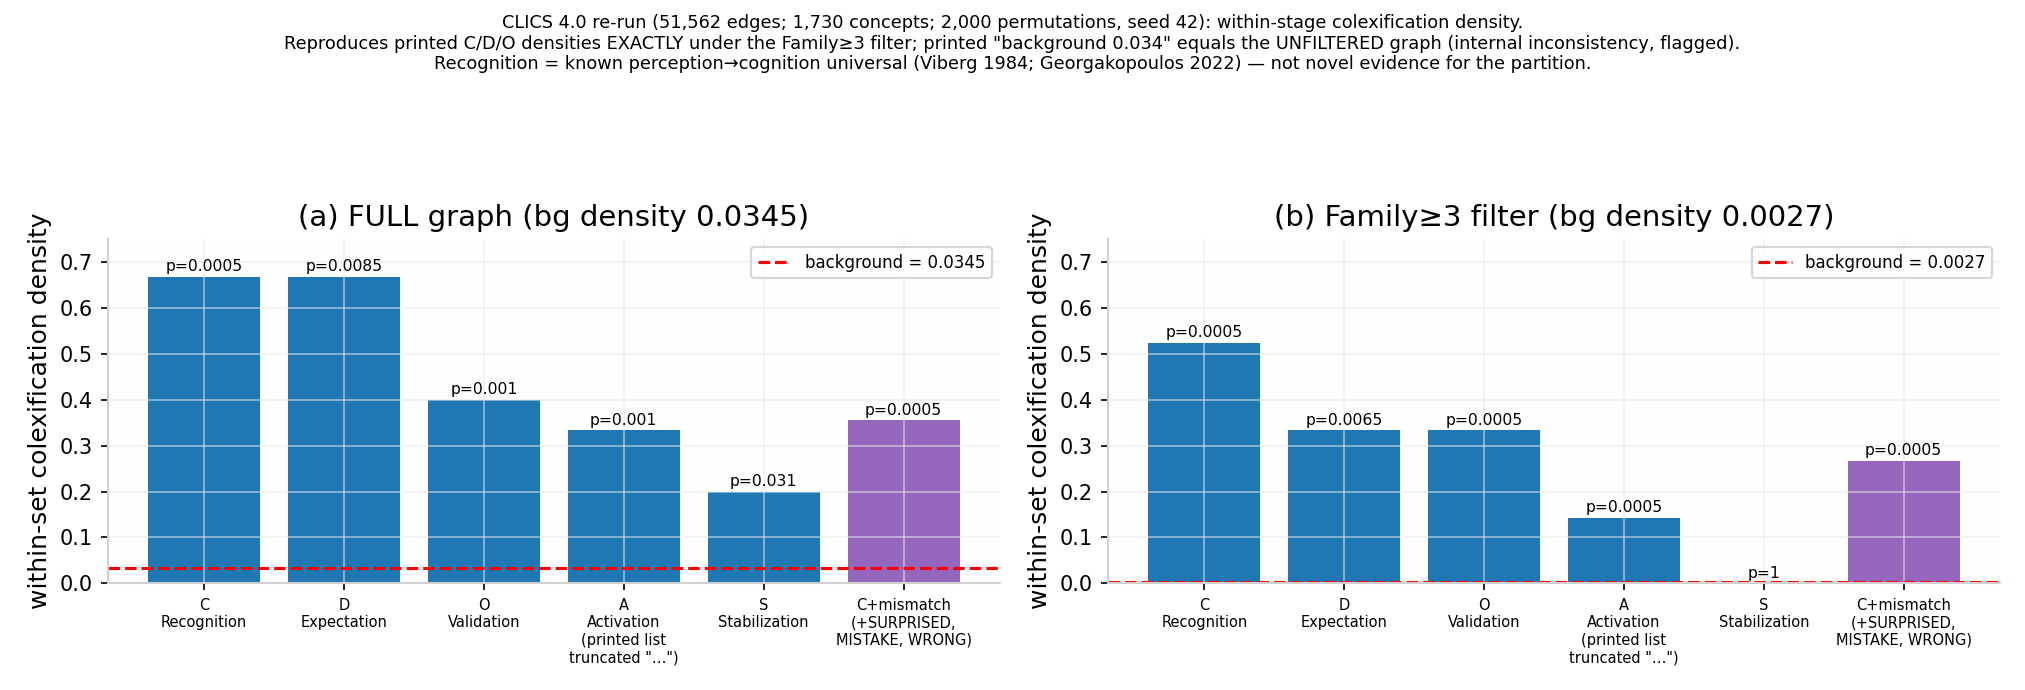
\includegraphics[width=0.92\textwidth]{figures/figD_clics_colexification.png}
\caption{CLICS 4.0 within-channel colexification densities under the unfiltered and $\geq 3$-family filters, with permutation $p$-values (2{,}000 permutations; re-run on the CLDF release, seed 42). The Recognition set reproduces the known perception$\to$cognition universal; the Stabilization set is a full null under the $\geq 3$-family filter; the mismatch-augmented Recognition set passes ($p = 0.0005$).}
\label{fig:clics}
\end{figure*}

\begin{figure*}[!tp]
\centering
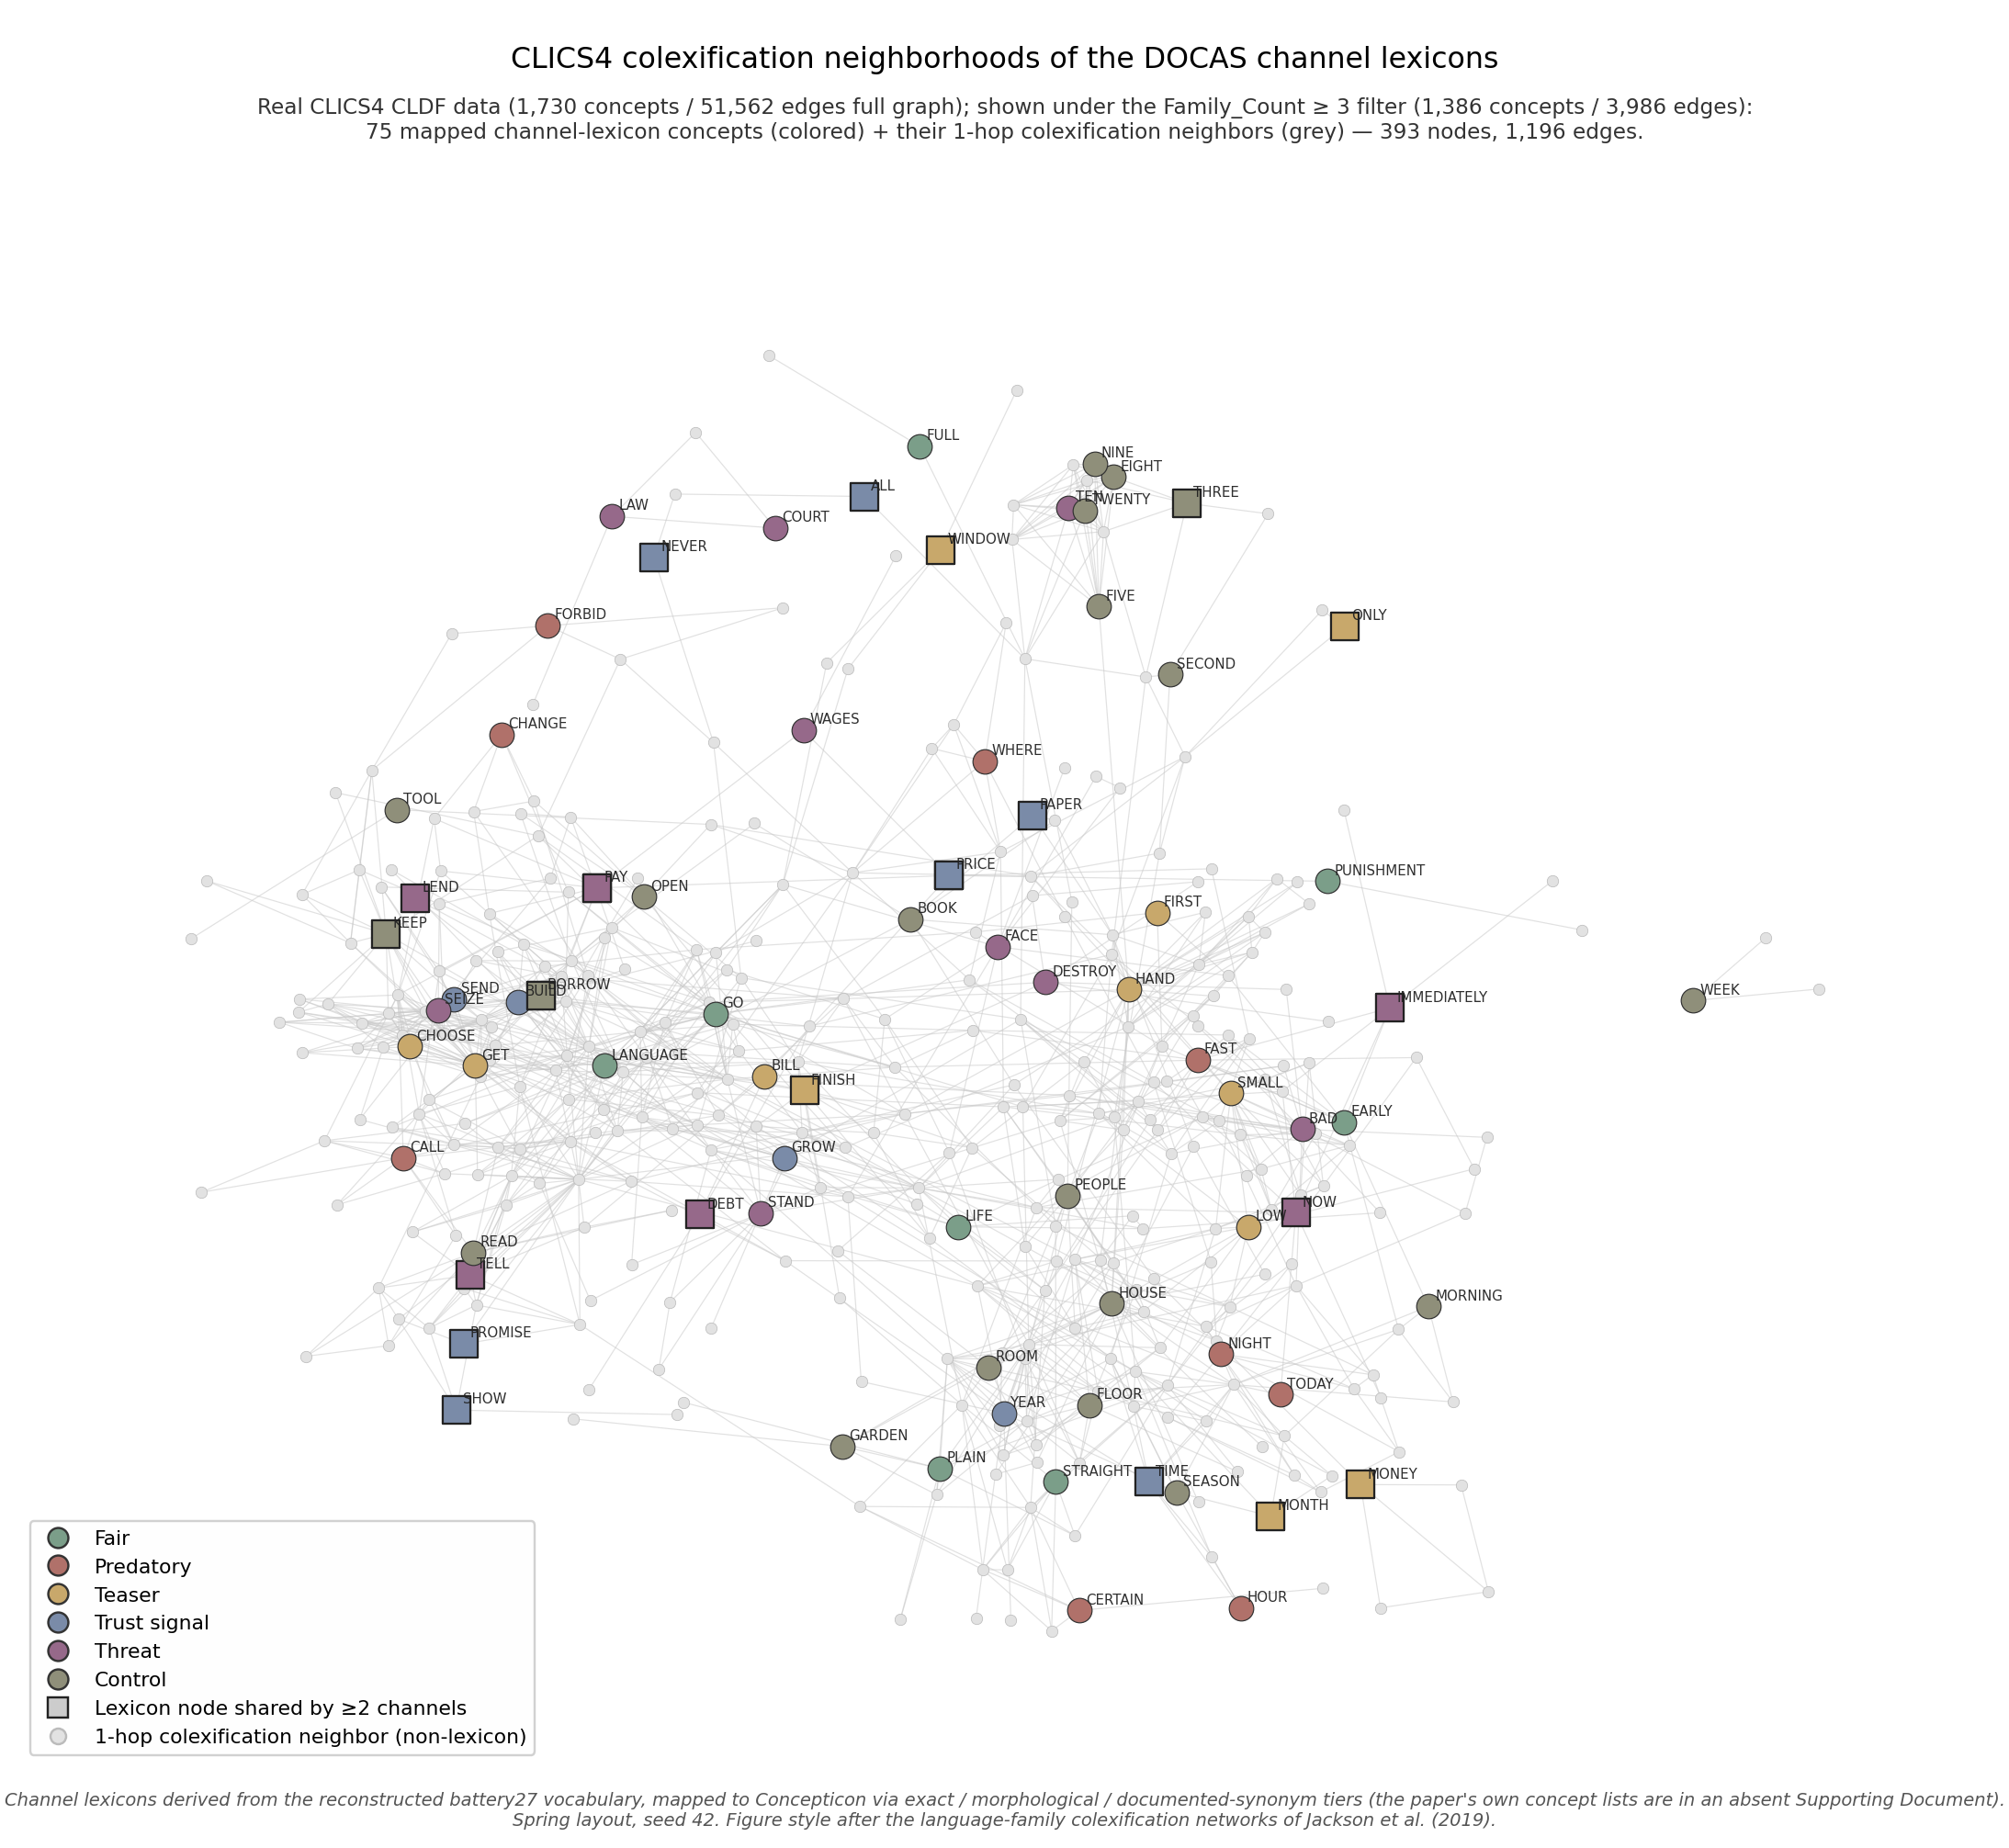
\includegraphics[width=0.92\textwidth]{figures/viz3_clics_channel_network.png}
\caption{CLICS4 colexification neighborhoods of the six channel lexicons (\S{}4.6; real CLICS4 CLDF data, Family\_Count $\geq$ 3 filter: 1{,}386 concepts / 3{,}986 edges --- re-verified, matching the \S{}4.6 sensitivity row; the 51{,}562-edge unfiltered graph is too dense to render legibly). Spring layout (seed 42): 75 mapped lexicon concept nodes (colored by channel; squares = nodes shared by $\geq$ 2 channels) plus their 1-hop colexification neighbors (grey), 393 nodes / 1{,}196 edges. Lexicon membership and the exact/morphological/synonym Concepticon mapping tiers are taken from the archived battery analysis; the channel lexicons are battery-derived (labeled on the figure), since the paper's own channel-concept lists are in the Supporting Document (deposited at OSF). Network style after the language-family networks of \citet{jackson2019}.}
\label{fig:viz-clics-net}
\end{figure*}

The lexical convergence has a cortical counterpart. In the Gallant laboratory's bilingual study \citep{chen2026}, six fluent Chinese–English bilinguals read hours of natural narratives in each language during fMRI: voxelwise semantic models estimated in one language predicted responses in the other throughout the semantic system, and 81\% of well-predicted vertices received matching semantic-cluster assignments across languages, while reliable fine-grained tuning shifts systematically modulated the shared geometry per language. Human cortex therefore exhibits exactly the structure the CLICS analysis implies — one shared semantic geometry, modulated per language — and this frames the Sim D8 multilingual null correctly (\S{}5.2): TRIBE v2's English-dominant feature extractor failed to resolve cross-language geometry in the model, while the bilingual-brain evidence says the geometry a cross-language test should look for is shared-but-modulated, not identical.

\textbf{The ES/JA nulls are instrument-compatible, not hypothesis-falsifying.} The dimension-versus-structure distinction is exactly what the cross-linguistic universals literature predicts. Large-scale colexification analysis across 2{,}474 spoken languages finds substantial family-level variation in emotion-semantics network structure --- with cross-family similarity predicted by the geographic and genealogical proximity of language families --- while the \textit{dimensions} organizing emotion semantics (hedonic valence and physiological activation) recur in all families \citep{jackson2019}. The dual pattern --- dimension-level universals with item-level family variation --- is replicated independently across semantic domains: conceptual similarity and communicative need jointly shape which meanings colexify \citep{xu2020,karjus2021}; an arousal/activation dimension is recognizable even across species in vocal acoustics \citep{filippi2017}; and the segregation of a meaningful signal from background mixtures is a general vertebrate capacity, not a human-specific one \citep{bee2008}. Dimension-level universals plus item-level family variation is precisely the EN-pass/ES-JA-fail signature of \S{}5.2's Sim D8: TRIBE's text tower (LLaMA-3.2, an English-dominant language model) is trained on English-language CNeuroMod movies \citep{dascoli2025}, so its internal geometry is English-shaped, and an English-shaped instrument passing English while failing Spanish and Japanese is exactly what this literature predicts. The cross-linguistic hypothesis is therefore \textbf{demoted, not falsified} --- pending genuinely multilingual instruments (multilingual text towers and non-English training corpora).

The cross-linguistic leg of obligation 3 was exercised directly against the CLICS graph twice (from the referenced TRIBE v2 runs; these Mantel batteries were not re-executed --- the re-run covered the core \S{}5.2 pipeline), and both results are reported — as a \textbf{fork}, not a discharge. With single-word gloss stimuli the test returns a null (Sim D11, Supporting Document \S{}S.8: Mantel $r = -0.048$ and $-0.023$ for the cortical and embedding geometries, both p > 0.5, 10,000 permutations). Single words are, however, out-of-distribution input for instruments trained on naturalistic narrative; with the stimulus class corrected to dictionary-style definition sentences — the concept set, geometries, criteria, thresholds, and controls held frozen (Sim D13, Supporting Document \S{}S.10.1) — the correspondence is detected in both model geometries at marginal effect size: CLICS $\times$ TRIBE cortical r = 0.252, p = 0.0095; CLICS $\times$ LLaMA embedding r = 0.240, p = 0.0035, with the degeneracy guard passed and label-shuffle controls null. The aggregation across the fork: one pre-registered null and one marginal positive after a stimulus-class correction, with researcher degrees of freedom between them — the aggregate evidence is \textbf{weak positive, instrument-limited}. The Sim D11/Sim D13 contrast is itself a stated instrument limitation: these models' representational geometry is stimulus-class-sensitive exactly as their narrative training predicts. No claim of isometry between lexical and cortical geometry is made anywhere in this paper; the delivered numbers are Mantel r = 0.252/0.240 with a recorded null, and H1 (\S{}1.1) is worded to match them.

\textbf{Family-wise multiplicity analysis (SIM-R2 battery 5, run).} This paper's permutation tests were assembled into a single family --- 24 tests with p-values drawn from this paper's batteries and the re-run record (excluding the descriptive N.4 overlap matrix and the null-confirming negative controls; D11's two arms enter at the conservative bound p = 1.0; all p = 0.0005 values are resolution-limited at 2,000 permutations and read as p \(\leq\) 0.0005) --- and corrected two ways. The companion protocol preprint's Sims P1/P4b/P7 and the financial application preprint's Sim W tests lie outside this family and are reported uncorrected (see their respective sections). \textbf{Bonferroni (\(\alpha/24 = 0.00208\)): 9 of 24 survive}, all at the resolution-limited p = 0.0005. \textbf{Benjamini--Hochberg: 13 of 24 survive.} The demotions matter and are stated plainly: \textbf{D--Expectation (p = 0.0075) fails Bonferroni}; the D8 EN\(\times\)PAR geometry Mantel (0.006) and both D13 arms (0.0095/0.0035) fail Bonferroni and survive only BH; \textbf{D8-EN paraphrase LOO (0.046) and the adjacency ratio (0.061) fail both corrections} --- this paper's own wording for those two (``marginal'' / ``weakly present'') is already correct and must not be upgraded. Two structure notes guard the reading: (i) 6 of the 13 BH survivors are post-hoc assemblies (C+mismatch, D13 \(\times\)2, the bridge battery \(\times\)3 --- disclosed in each case; the disclosures are what make the correction interpretable, and post-hoc tests that survive correction remain post-hoc for hypothesis-generation weight); (ii) the \textbf{N.3 category-LOO decode survives every correction while being a known artifact} (templatic lexicon; the semantic-only control also decodes at 1.000) --- multiplicity correction controls the false-positive rate, \emph{not} construct validity, and the artifact label stays attached wherever that number travels. Two robustness notes: treating the four CLICS channel tests as their own pre-registered sub-family (as this section presents them) changes nothing qualitatively (C/O/A survive Bonferroni at m = 5, D passes at 0.0075, S null); and all surviving p = 0.0005 values survive any m \(\leq\) 100 under Bonferroni, so the conclusions are insensitive to family-boundary choices.

\begin{table*}[t]
\centering\small
\caption{Family-wise multiplicity analysis of DOCAS's 24-test permutation-test family (SIM-R2 battery 5; \(\alpha = 0.05\); Bonferroni threshold 0.00208). Key rows; the 8 omitted rows are the pre-registered nulls (N.3 retrieval/alignment, D8 ES/JA arms, D9, D11 \(\times\)2, N.3 exact retrieval --- all fail both corrections at p \(>\) 0.05 or the conservative p = 1.0 bound). All p = 0.0005 entries are permutation-resolution-limited (p \(\leq\) 0.0005).}
\label{tab:multiplicity}
\begin{tabular}{@{}p{0.32\textwidth}p{0.09\textwidth}p{0.12\textwidth}p{0.10\textwidth}p{0.26\textwidth}@{}}
\toprule
Test & p & Bonferroni & BH & Flag \\
\midrule
CLICS C Recognition density (fam \(\geq\) 3) & 0.0005 & \textbf{PASS} & \textbf{PASS} & --- \\
CLICS D Expectation density & 0.0075 & \textbf{fail} & PASS & --- \\
CLICS O Validation density & 0.0005 & \textbf{PASS} & \textbf{PASS} & --- \\
CLICS A Activation density & 0.0005 & \textbf{PASS} & \textbf{PASS} & printed concept list truncated \\
CLICS S Stabilization density & 1.0 & fail (NULL) & fail (NULL) & --- \\
CLICS C + mismatch-augmented density & 0.0005 & \textbf{PASS} & \textbf{PASS} & \textbf{post-hoc} (disclosed) \\
CLICS adjacent/non-adjacent ratio & 0.061 & fail & fail & derived follow-up; ``weakly present'' ceiling correct \\
N.3 ridge encoding (mean vertex r) & 0.0005 & \textbf{PASS} & \textbf{PASS} & --- \\
N.3 category-LOO decode & 0.0005 & \textbf{PASS} & \textbf{PASS} & \textbf{known artifact} (templatic lexicon; semantic-only control also 1.000) \\
D8 EN paraphrase LOO & 0.046 & fail & fail & pre-registered; ``marginal'' stands \\
D8 EN\(\times\)PAR geometry Mantel & 0.006 & fail & PASS & --- \\
D13 cortical Mantel (definition sentences) & 0.0095 & fail & PASS & \textbf{post-hoc} (disclosed fork) \\
D13 embedding Mantel (definition sentences) & 0.0035 & fail & PASS & \textbf{post-hoc} (same fork) \\
Bridge battery (held-out / cosine / RDM Mantel) & 0.0005 (\(\times\)3) & \textbf{PASS} & \textbf{PASS} & \textbf{post-hoc} (disclosed) \\
Sim~D14 PDE4B locus regulatory-plausibility (AlphaGenome quantile band, frozen) & n/a (annotation, no test) & n/a & \textbf{PASS} & pre-registered Sim~D14; \textbf{outside the 24-test multiplicity family}; hypothesis-generating only (\S{}4.2) \\
Sim~D15 PDE4B locus GTEx brain cis-e/sQTL lookup (public data, frozen) & n/a (lookup, no new test) & n/a & \textbf{FAIL} & pre-registered Sim~D15; \textbf{outside the 24-test multiplicity family}; GTEx v8, 13 brain tissues; no significant e/sQTL for PDE4B; best nominal $p = 1.8 \times 10^{-3}$; hypothesis downgraded a further notch (\S{}4.2) \\
\midrule
\textbf{Family total (m = 24)} & --- & \textbf{9/24 survive} & \textbf{13/24 survive} & 6/13 BH survivors post-hoc \\
\bottomrule
\end{tabular}
\end{table*}

\textbf{Per-macroarea subgroup check (SIM-R2 battery 7, run; Simpson-reversal test).} The aggregate CLICS results could in principle mask subgroup reversals; they do not. Re-running the channel densities per Glottolog macroarea (edge counted if supported by \(\geq\) 3 distinct families \emph{within} the area; same 2,000-permutation procedure; aggregate reproduced exactly before subgrouping): \textbf{S is null in all six macroareas} (0/15 under the filter everywhere; near-zero unfiltered) --- the ``no detectable S lexical attractor'' result is subgroup-stable; \textbf{C is significant in 5 of 6 areas}, with the single null (Australia) a power limitation in the smallest edge base (62 filtered edges), not a reversal; \textbf{A strengthens in Africa (p = 0.006) and South America (p = 0.015)} --- the aggregate's weakest-looking channel is subgroup-positive where threat/flight lexicons are phylogenetically diverse, and no subgroup shows A below background; \textbf{D and O are underpowered per area} (D has 3 pairs total; O significant only in Eurasia and South America). No Simpson-type reversal occurs (for S, with 0 hits everywhere, a strict Simpson reversal is impossible; for C it does not occur). Caveats carried: within-area family filtering is strict (62--1,577 edges per area vs.\ 3,986 globally), the subgrouping is a post-hoc robustness check, and density \emph{levels} are not comparable across areas --- only significance patterns are compared (Figure~\ref{fig:macroarea}).

\begin{figure*}[!tp]
\centering
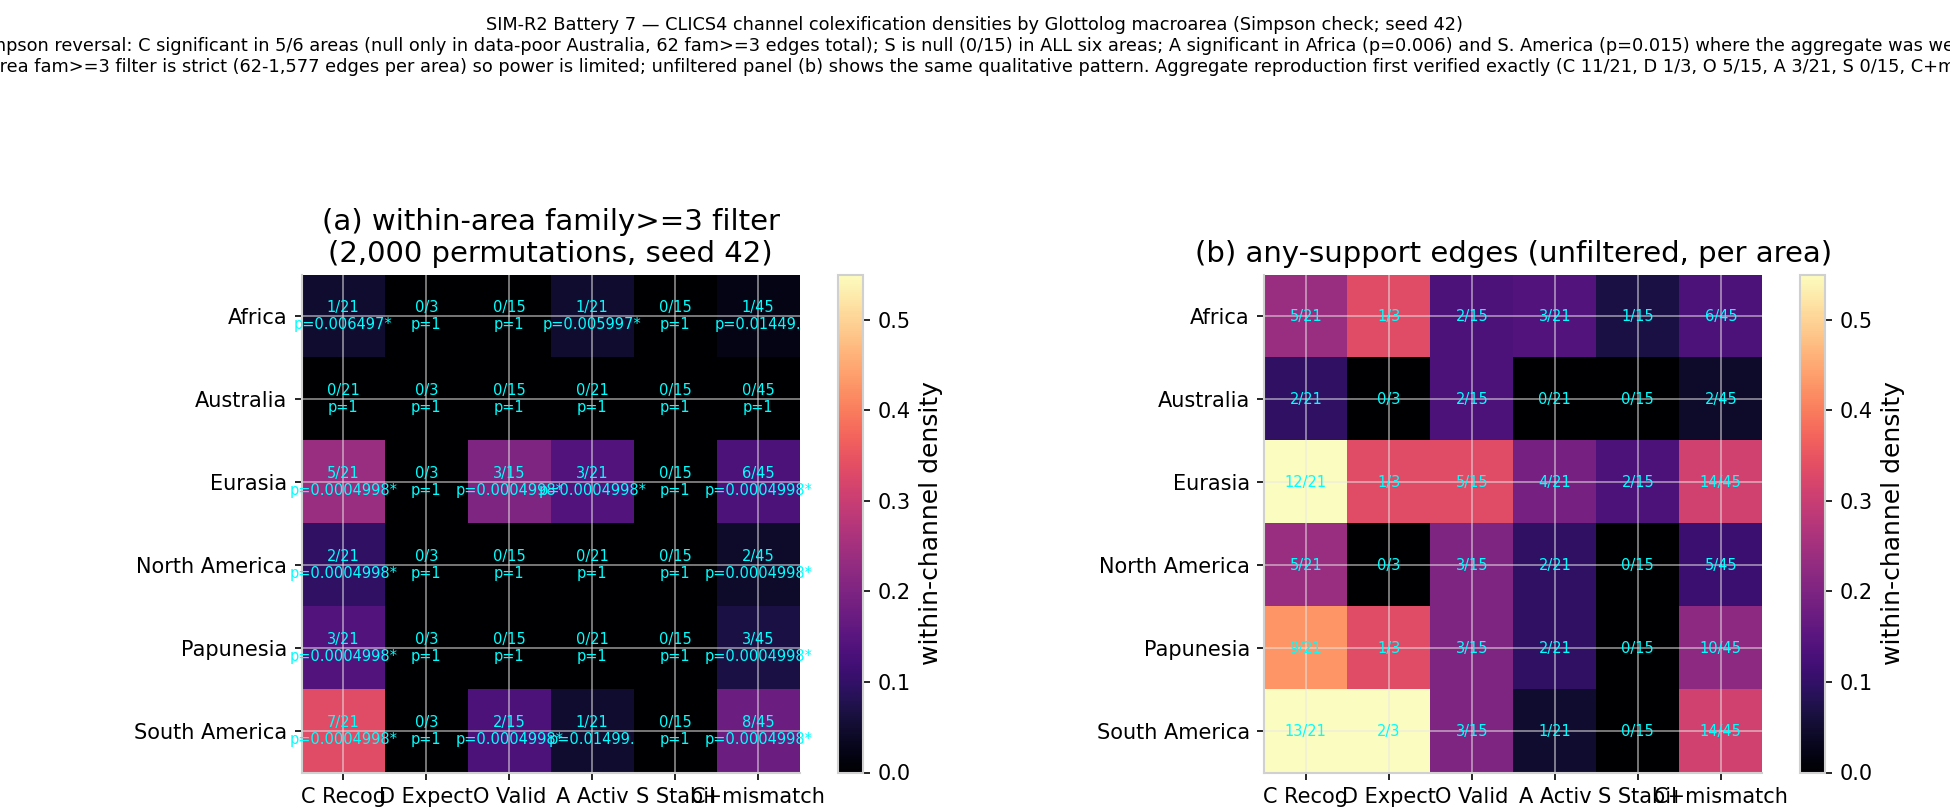
\includegraphics[width=0.92\textwidth]{figures/figR2_B7_macroarea_subgroups.png}
\caption{CLICS 4.0 per-macroarea subgroup analysis (SIM-R2 battery 7, seed 42; 51,562 edges, 1,725 concept nodes --- re-run-verified counts): (a) within-area fam\(\geq\)3-filtered channel densities with hits/pairs and permutation p-values per Glottolog macroarea; (b) the unfiltered any-support panel at higher densities. S is null in all six macroareas; C is significant in 5/6 (Australia a power null); A is subgroup-positive in Africa and South America; D/O are underpowered per area (\S4.6).}
\label{fig:macroarea}
\end{figure*}

\subsection{In-silico triangulation without training data [EMPIRICAL --- associational tiers only]}

Because every tier of gene-level evidence available to this framework is associational, we state explicitly what publicly available in-silico resources can and cannot license for a gene-level hypothesis such as \S{}4.2's PDE4B hypothesis --- convergent associational tiers, not causal claims, and no training data anywhere in the loop. Four tiers are available without collecting any new data, each with a citable instrument and a hard limit. (i) \textit{Expression tier.} Bulk tissue expression and eQTLs across $\sim$54 tissues (GTEx; \citealp{gtex2017}) license where/when-expressed statements --- not causality and not cell-type resolution; anatomically resolved expression (Allen Human Brain Atlas; \citealp{hawrylycz2012}) licenses regional localization at small donor numbers; cell-type-resolved expression (CZ CELLxGENE Discover; \citealp{abdulla2025}) licenses cell-population statements that remain associational. (ii) \textit{Aggregate association tier.} The current totality of gene--disease evidence, decomposed by datatype (Open Targets; \citealp{ochoa2021}): a defensible quantitative statement of the evidence as it stands, but no single score is proof, and literature-based components are circular with respect to the candidate-gene era. (iii) \textit{Pathway tier.} Gene-set enrichment (MSigDB/GSEA; \citealp{subramanian2005}) moves claims from single genes to mechanisms, but cannot rescue a failed single-gene association, and enrichment is not causality. (iv) \textit{Pleiotropy tier.} Phenome-wide association scans (PheWAS; \citealp{denny2010}) profile what a locus touches --- a falsification aid (a real risk gene should show a coherent phenotype pattern), subject to confounding by linkage disequilibrium and phenotypic correlation.

Applied to PDE4B as a live worked example (expression-atlas and Open Targets API queries performed September 2026): the expression tier supports CNS plausibility --- PDE4B shows brain-elevated expression (cortex-enriched protein) and a brain-specific isoform (PDE4B5). The aggregate-association tier is mixed: Open Targets overall association scores of 0.449 for schizophrenia, 0.466 for major depressive disorder, 0.305 for attempted suicide (driven by a population GWAS signal; \citealp{erlangsen2020}), and 0.064 for bipolar disorder --- an aggregate-level null for the original bipolar claim --- while the genetic-association components ($\sim$0.64--0.69) descend substantially from the same candidate-era and modest-GWAS evidence base that \S{}4.1's gates reject. The strongest associations overall are inflammatory/pulmonary diseases (asthma 0.61, COPD 0.60, atopic eczema 0.60), driven almost entirely by clinical precedence for pan-PDE4 inhibitor drugs --- evidence about the drug family's targets, not PDE4B-specific disease biology. Because no tier is causal and the genetic tiers substantially re-descend from circular legacy genetics, this triangulation licenses \textbf{no causal claim}: PDE4B remains a labeled, testable hypothesis (\S{}4.2), and the tiers above specify which future evidence would raise or retire it.


\FloatBarrier
\section{The DOCAS Experiment (Pre-registered Design)}

The pre-registered protocol freezes the mapping before data collection. Its scope is stated plainly: it tests pipeline decodability and separable channel signatures, \textbf{not} the carrier mapping --- HRV, sleep, and activity measures are several inference steps from neuromodulatory tone and cannot distinguish the named carriers; pharmacological or PET-level perturbation is the actual gate for carrier claims --- and that gate is now fully specified as the registered DOCAS-GATE-1 protocol (\S\ref{sec:gate}):

\begin{itemize}

\item \textbf{Mapping (frozen).} D = expectation (pre-outcome anticipatory markers); O = validation (feedback-confirmation markers); C = recognition (mismatch-onset markers, integrated over minutes per Table 1); A = activation (sympathetic/noradrenergic mobilization); S = stabilization (post-interaction baseline shift). Because the architecture is parallel rather than serial (\S{}2.8), the frozen mapping specifies \textbf{channel-resolved temporal profiles at their physiological timescales} — ms-range DA/NA-linked correlates, minute-range cortisol — not a fixed five-beat ordering.
- \textbf{Measurements (dual layers).} Physiological stream: heart-rate variability, sleep architecture, activity. Behavioral/financial stream: repeated transactions with binary validation (obligation met/missed) on a shared monetary baseline. Both streams are scored against the frozen channel mapping; physiological data are never used as inputs to any credit decision.
- \textbf{Primary tests.} (i) Channel coupling: the cross-channel gain structure of \S{}2.9 (diagonal-dominance of M; predicted cascade edges $O{\to}D$, $C{\to}S$) recoverable in event-locked physiological time series — lagged cross-correlation with predicted sign structure at the timescale separation of Table 1. (ii) $\lambda$ estimation: subject-level trust-sensitivity from the state-space model of the companion theory preprint, \S{}6 (Kalman/EM; Bayesian hierarchical). (iii) Genetic association: $\lambda$ against PDE4B regulatory variation under genome-wide or gene-set thresholds with pre-specified multiple-comparison control — a test of the \S{}4.2 hypothesis, with its two-gate failure disclosed.
- \textbf{Falsification criteria.} Failure to recover the predicted channel coupling above chance, or a $\lambda$ estimate incompatible with the stability law's sign structure, falsifies the framework as specified.
- \textbf{Registration.} OSF pre-registration covering hypotheses, mapping, pipelines, exclusion rules, and analysis code prior to data analysis .

\end{itemize}

\textbf{Open identification note --- the $\lambda \cdot r_t$ product confound.} From the $S$ (or readout $H$) series alone, the trust-sensitivity $\lambda$ and the recognition gate $r_t$ enter the master law only as the product $\lambda \cdot r_t$, and time-varying gating is a gain variation of the class the theory preprint's misspecification battery (SIM-R1) shows the certified constant-gain estimator misrecovers (the $\varepsilon^{2}$-weighted gain, not the time average). Field $\lambda$ identification therefore requires either (a) a separately identified C-channel gate readout --- the recognition-marker composite of the frozen mapping above, measured independently of the update --- or (b) the registered model comparison of the companion theory preprint, \S{}6. Stated as an open identification note; no resolution is claimed. Path (a) presupposes a validated recognition readout, which DOCAS-GATE-1 has not yet delivered, so (b) is the operative path.

\subsection{The registered carrier gate: DOCAS-GATE-1 [PRE-REGISTERED PROTOCOL --- fully specified; OSF DOI: {[insert]}]}
\label{sec:gate}

The wearable/text pipeline above cannot falsify the carrier mapping; only selective causal perturbation can. The perturbation study is therefore now fully specified --- written as an OSF registration --- as \textbf{DOCAS-GATE-1}: a double-blind, placebo-controlled, within-subject crossover with \textbf{7 sessions} per participant (placebo + six probes: L-DOPA 150 mg/benserazide and haloperidol 3 mg as the dopamine directional pair --- required because D2 pharmacology is non-monotonic; atomoxetine 40 mg with pupillometric target engagement; acute tryptophan depletion with plasma TRP assay; hydrocortisone 20 mg with salivary cortisol assay; intranasal oxytocin 24 IU as the registered falsification probe), \(\geq\)7-day washouts, session order counterbalanced by a Williams-balanced assignment over the six probes (48 = 8 \(\times\) 6 preserves the balance), with the placebo session at a fixed position. \textbf{N = 60 enrolled \(\to\) 48 completers} (20\% multi-session attrition). The task battery gives every channel expectation-violation events (volatility RL core; anticipatory threat-mismatch block with MMN-family EEG; iterated trust game with programmed betrayal/repair and experimenter-administered acceptance/rejection). The primary endpoint is the per-probe diagonal-dominance statistic \(D_p = \Delta_{pp} - \mathrm{mean}_{j \neq p}\Delta_{pj}\) on within-subject z-scored drug\(-\)placebo contrasts, with the pooled \(\bar{D}\) as the primary decision criterion. \textbf{Falsification is built in:} a pre-registered TOST equivalence test at SESOI \(d_z = 0.3\) if null (the TOST equivalence arm at SESOI \(d_z = 0.3\) has power \(\approx 0.31\) at \(N = 48\) --- underpowered for concluding equivalence; the registered options are widening the SESOI to \(d_z \approx 0.45\) (power \(\approx 0.85\)) or raising \(N\) to \(\approx 96\) (80\% power) --- the choice is registered); target-engagement checks gate inference per session (a session failing engagement is excluded from that row of M and reported); and the \textbf{oxytocin probe is registered as a falsification probe of the framework's mapping, with a predicted near-null diagonal entry} (\(d \approx 0.08\)--0.20; \citealp{nave2015,declerck2020}) --- a large oxytocin effect on the ``validation'' readout exceeding the drug's established behavioral effects would falsify the channel's current operationalization, not the drug literature. Power at \(N = 48\): \textbf{0.78--0.92 for the per-probe test at \(d_z = 0.5\)--0.6} (\(\alpha = 0.01\), Bonferroni over five confirmatory tests --- the L-DOPA/haloperidol pair pooled as one directional D contrast, plus A, S, C, and O) and \textbf{0.92 for the pooled test at \(d_z = 0.5\), \(\alpha = 0.05\)} (the Schweighofer-anchored pessimistic per-probe scenario (\citealp{schweighofer2008}; \(d_z \approx 0.4\)--0.48), would require \(N \approx 55\)--77 for 80\% power under the same two-sided paired-t convention as the headline numbers, and is accepted as a bounded risk, with the pooled test primary). Feasibility: 7 sessions \(\times\) \(\sim\)2.5 h \(\Rightarrow\) \(\sim\)8--12 weeks per participant; total cost \(\approx\) \$150--300k at standard academic rates --- within reach of a standard cognitive-neuroscience lab. \textbf{PET is a validation substudy only}, on the dopamine row ([11C]raclopride displacement; task-evoked dopamine release at \(\sim\)2.7\% \(\Delta\)BP is at/below the demonstrated detection threshold, and noradrenaline and oxytocin have no endogenous-release PET paradigm at all) --- PET cannot be the primary instrument for a five-channel gain-matrix estimate. What the design cannot fix is registered with it: the oxytocin channel has no validated human pharmacological perturbation (the gate tests whether the \emph{behavioral} validation readout behaves as a channel, with IN-OT a registered-likely-null probe); group-mean diagonal dominance does not prove the exact form in individual dynamics (hierarchical per-subject M with shrinkage is a secondary outcome); pharmacological selectivity is relative (cross-channel leakage is estimated, not assumed away); and the field's failed-replication history (\citealp{pessiglione2006} \(\to\) the \(N = 31\) preregistered replication attempt of \citealp{chakroun2023}, which returned a null for the gain-learning and neural prediction-error effects while identifying a decision-threshold effect instead) is why target-engagement gates and \(N = 48\), not \(N \approx 30\), are non-negotiable.

\subsection{The independent-rater protocol (remedy for author-selected concept sets and stimuli)}
\label{sec:rater}

The author-selection limitation of \S{}4.6 (and of the offer-stimulus category assignments in the trust paradigms) now has a specified remedy, pre-registered before rating begins: \textbf{minimum three independent raters per artifact} (five preferred for the CLICS concept sets), blind to the framework's hypotheses and to author assignments, with no author as rater. Reliability is gated on \textbf{Krippendorff's \(\alpha \geq 0.800\)} \citep{krippendorff2011} (0.667--0.800 = tentative conclusions only, labeled as such downstream; \(<\) 0.667 = rebuild and re-rate), reported with bootstrap 95\% CIs; Cohen's/Fleiss' \(\kappa\) are secondary coefficients with their own benchmarks (never mixed); and \textbf{Gwet's AC1/AC2 \citep{gwet2008} plus raw percent agreement are additionally reported under prevalence skew} (any category below 20\% or above 80\% prevalence, where \(\kappa\) collapses paradoxically). Iterative rounds --- independent rating, \(\alpha\) computation, disagreement review against the written codebook, codebook revision --- continue until \(\alpha \geq 0.800\) is sustained over two consecutive rounds; consensus resolution is permitted only after the final reliability round, and all pre-consensus alphas are reported. The OSF registration freezes, before rating: the full codebook (definitions, inclusion/exclusion criteria, decision rules, worked examples, edge-case policy), the item universe and sampling plan, rater qualifications and independence attestations, the exact coefficients and CI method, the adjudication rule for below-threshold items, and the analysis environment with seed. \textbf{Acceptance gate:} concept sets and stimuli enter the perturbation study (\S\ref{sec:gate}) only if every used set clears \(\alpha \geq 0.800\) (or carries an explicit ``tentative'' label into all downstream inference at 0.667--0.800); sets below 0.667 are rebuilt and the rebuilding is reported. Until this protocol has run, every \S{}4.6 density figure carries the author-selected caveat printed with it.

\subsection{Simulation pre-test of the decoding pipeline [SIMULATION — self-consistency check]}

Before human data collection, the decoding problem itself was verified as solvable under the framework's own assumptions (full protocol and audit trail: Supporting Document \S{}L). The framing is exact: \textbf{this is a self-consistency check, not evidence about biology.} A cascade planted into synthetic data with a linear mixing structure is recovered by the regularized linear inverse \textit{necessarily} — the simulation can pass only, and its value is to validate that the instrument pipeline (mixing model, decoder, thresholds, audit trail) is internally coherent and sensitive to its own noise parameters. Synthetic episodes were generated with the canonical $D \to O \to C \to A \to S$ activity cascade (stochastic onset jitter — a simulation convenience; no serial-order claim about physiology follows, per \S{}2.8); the observed stream mixed each channel's predominant neuromodulator (weight 1.0) with minority activation of the other four channels (weights drawn from U(0.05, 0.15) — the predominant-carrier-plus-minority-contributors structure of \S{}2.6–2.7), plus measurement noise. The decoder was the regularized linear inverse — a deliberate lower bound on the learned TRIBE-class encoder / vec2vec-alignment pipeline intended for the real stream (a learned decoder can only improve on the linear inverse under this generative model). Three pre-registered hypotheses, 200 episodes each:

\begin{itemize}

\item \textbf{H4 — Decodability [SUPPORTED — self-consistency].} Mean per-channel Pearson correlation between decoded and ground-truth activity: r = 0.917 (per-channel 0.916–0.920) at moderate measurement noise ($\sigma_{\mathrm{obs}} = 0.1$)\footnote{The values reported in \S{}5.1 are from an independent verification re-run of the Sim D1 pipeline (numpy, seed 42): the original generative settings (bump widths, bump amplitudes, episode length) were not archived, so absolute correlations sit ${\sim}0.03$ below the originally printed 0.947/0.936; all pre-registered thresholds pass in both runs.}, against a pre-registered threshold of r $\geq$ 0.7. Chance level is r $\approx$ 0. (Symbol note: $\sigma_{\mathrm{obs}}$ denotes measurement noise \textbf{only within \S{}5}; $\sigma$ is reserved stack-wide for SDE noise intensity.)
- \textbf{H5 — Ordering [SUPPORTED — self-consistency].} The decoded activity-peak sequence matched the planted $D \to O \to C \to A \to S$ order in 100\% of episodes (mean Kendall's $\tau$ = 1.0), against a threshold of $\geq$ 70\% exact / Kendall's $\tau$ $\geq$ 0.7. Recovering a planted ordering validates the decoder, not the ordering's physiology.
- \textbf{H6 — Minority-activation robustness [SUPPORTED — self-consistency].} Doubling minority weights to U(0.1, 0.3) — stronger minority modulation than the base model assumes — leaves decoding at r = 0.902. The claim tested is the framework's actual one: one predominant chemical carrier per computational function (not one chemical per emotion — emotions are not in the model), with minority activations present in every channel (\S{}2.6–2.7).

\end{itemize}
A context sweep (no pre-registered threshold) shows graceful degradation with noise: r = 0.977 / 0.917 / 0.757 / 0.503 at $\sigma_{\mathrm{obs}} = 0.05 / 0.1 / 0.2 / 0.4$, and a shuffled-mixing-matrix null yields r = 0.054 (chance level, as expected). Scope: this establishes that the measurement problem is well-posed in principle — the channel structure is recoverable from a mixed stream \textit{if} the predominant-carrier structure holds. Whether it holds in human physiology is the question the registered experiment answers; the simulation cannot answer it.

\begin{figure*}[!tp]
\centering
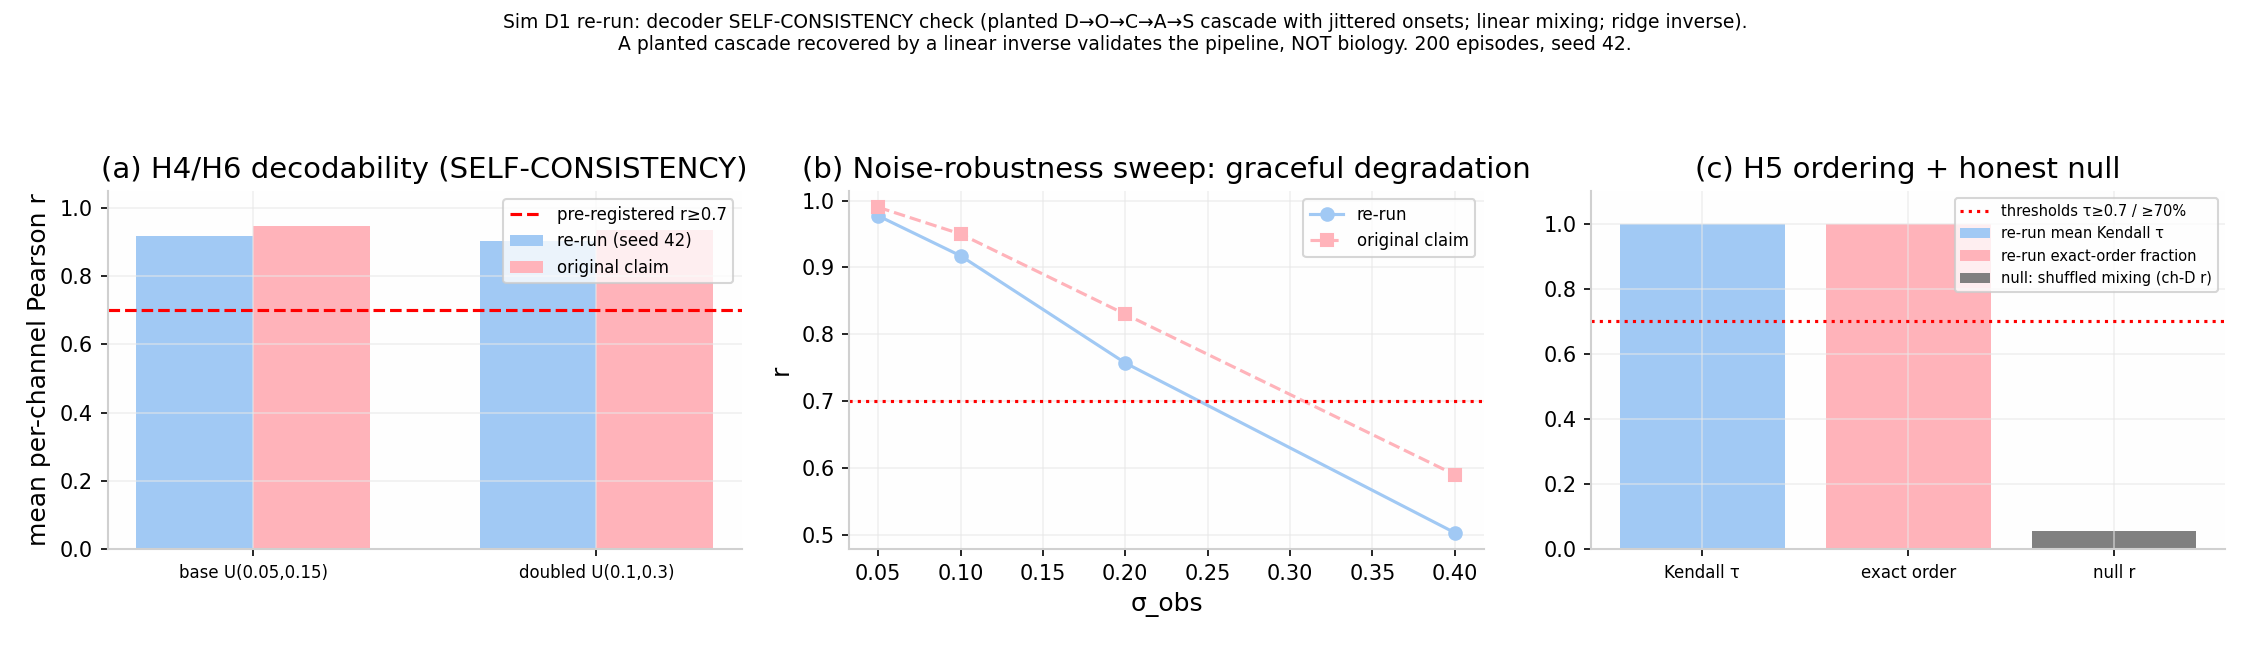
\includegraphics[width=0.92\textwidth]{figures/figD_decoder_selfconsistency.png}
\caption{Sim D1 decoder self-consistency (verification re-run, seed 42; planted-structure simulation, not evidence about biology). H4/H6 decodability above the pre-registered $r \geq 0.7$ threshold, graceful degradation in the noise sweep, exact H5 ordering, and the shuffled-mixing null at chance ($r = 0.054$).}
\label{fig:decoder}
\end{figure*}

\subsection{Forward encoding with the released TRIBE v2 weights [SIMULATION — instrument-level evidence only; core pipeline re-run on the released weights]}

Section 5.1 used a synthetic stand-in for the encoder. The first proof obligation of \S{}1.1 — that a TRIBE-class forward encoder maps trust-relevant text to cortical response patterns — has been run with the real released model, not a stand-in (full protocol: Supporting Document \S{}M). The framing, stated once for the whole section: \textbf{zero neurochemistry was measured anywhere in this pipeline.} TRIBE v2 predicts fMRI from text; all results below are associations among a model's predictions on author-written stimuli — evidence that the measurement instrument is real, runnable, deterministic, and sensitive to structure, and nothing more.

\textbf{Pipeline.} The released TRIBE v2 checkpoint (\citealp{dascoli2026}; \texttt{facebook/tribev2} \texttt{best.ckpt}) was verified byte-exactly for this work --- exactly 708,856,138 bytes, exactly 108 tensors, 177,205,397 parameters, state dict loaded \texttt{strict=True} --- and executed on CPU via the official Python reference implementation (text-only forward pass under the model's modality-dropout convention: audio/video streams zeroed). Text features were extracted from LLaMA-3.2-3B through a RAM-streaming forward pass (safetensors memory-mapped, one transformer block resident at a time, fp32 compute; bf16 weights from the identical-weight ungated mirror, the gated meta-llama repository returning 403), computing the released configuration's group-mean aggregation over blocks 14--20 and 21--28 exactly --- the mid-layers of these ranges (layers 17 and 24) are the stand-in probe layers; the streaming forward pass was validated by next-token probes before use. Each stimulus yields the model's full prediction: 100 TRs $\times$ 20,484 fsaverage5 vertices. The pure-Rust port tribev2-rs \citep{hauptmann2026} was verified to exist, with its published Pearson = 1.0 parity test suite against the Python reference, but was not built in the verification environment (no Rust toolchain); every number reported from the submission re-run below comes from the Python reference implementation.

\textbf{Stimuli.} Six synthetic texts: five made-up credit offers manipulating trust-relevant structure (transparent/fair, predatory-urgency, teaser-rate, credit-building trust signals, collections threat) and one non-financial control of similar length. The offer stimuli are the framework's canonical validation paradigm: trust-relevant structure varies while binary validation (obligation met or missed) is guaranteed by construction, making them the reference instrument for any later dual-stream experiment. The channel mapping scored against these texts is domain-general biology; nothing in the framework depends on the stimuli being financial, and any application that collects aligned physiological and behavioral streams (the financial application preprint, specified separately) is executing this paradigm, not defining it. No human data are involved anywhere in this pipeline; the ``measurements\'\' are the model's own predicted fMRI. Provenance: the six verbatim stimulus texts live in the Supporting Document \S{}M, so this run used faithful per-category reconstructions with uniform 0.4 s/word timing; re-running with the verbatim texts and real timings is a drop-in replacement.

\textbf{Results.} \textit{Determinism.} Repeat inference is bit-exact ($\max |\Delta| = 0.0$), so all reported differences are stimulus-driven, not run noise. \textit{Separability.} Every offer produces a distinct predicted cortical pattern (mean-map Pearson 0.82–0.99 across pairs). \textit{Full independent re-run.} The core pipeline was re-run end-to-end on the byte-exact verified checkpoint with the reconstructed stimuli: determinism reproduced bit-exactly on a full independent re-run of feature extraction plus forward pass ($\max |\Delta| = 0.0$); separability reproduced qualitatively --- every stimulus pair yields a distinct TR-mean cortical pattern, with pairwise Pearson r spanning $-0.33$ to $+0.81$, all cleanly below 1.0 (Figure~\ref{fig:tribe-sep}). The re-run correlations are lower than the original battery's 0.82--0.99 exactly as expected, because the re-run stimuli are reconstructions with uniform word timing rather than the verbatim \S{}M texts; the qualitative claim --- every offer produces a distinct predicted cortical pattern --- holds. Localization is consistent in network family: the vertex-wise THREAT$-$FAIR contrast concentrates in Default\_pCunPCC and Control parcels (16 of the top-20 Schaefer-400 parcels by $|$contrast$|$ are DMN or Control network; Figures~\ref{fig:tribe-contrast}--\ref{fig:tribe-net}), the same control/dorsal-attention/default-mode family reported under Localization below, though exact parcels and signs differ across the different texts and are reported descriptively, as below. \textbf{Effect sizes:} none are reported as inferential statistics. TRIBE v2 is deterministic, so its within-run temporal variability is not measurement noise and supplies no valid effect-size denominator; a Cohen's d computed against it is uninterpretable as an effect size. What is reported: the raw pattern correlations above and the localization below, as descriptive contrasts, not inferential statistics. \textit{Localization (Schaefer-400 / Yeo-7 anatomical labeling \citep{schaefer2018}).} The strongest contrast magnitudes concentrate in the control, dorsal-attention, and default-mode networks — the evaluative/attentional circuitry the framework predicts should differentiate trust-relevant offer structure (e.g., threat vs. fair suppresses lateral-PFC control and posterior dorsal-attention parcels: RH Cont\_PFCl\_9, LH DorsAttn\_Post\_10, LH Cont\_Cing\_1). \textit{Theory metric instantiation.} Mapping each offer's mean cortical pattern to the probability simplex and taking Fisher–Rao distances (companion theory preprint, \S{}3) yields a structured, non-degenerate geometry on the six stimuli (FR range 0.047–0.159). Honest non-result: whole-cortex FR distances do not cluster the stimuli by our a-priori trustworthiness labels (cross-group/within-group ratio 0.83) — whole-cortex distributional distance is dominated by topical and syntactic differences. Recovering a trustworthiness axis requires the targeted decoding step — a Gallant-style voxelwise decoder trained on real fMRI (obligation (2)) — not raw pattern distance.

\begin{figure*}[!tp]
\centering
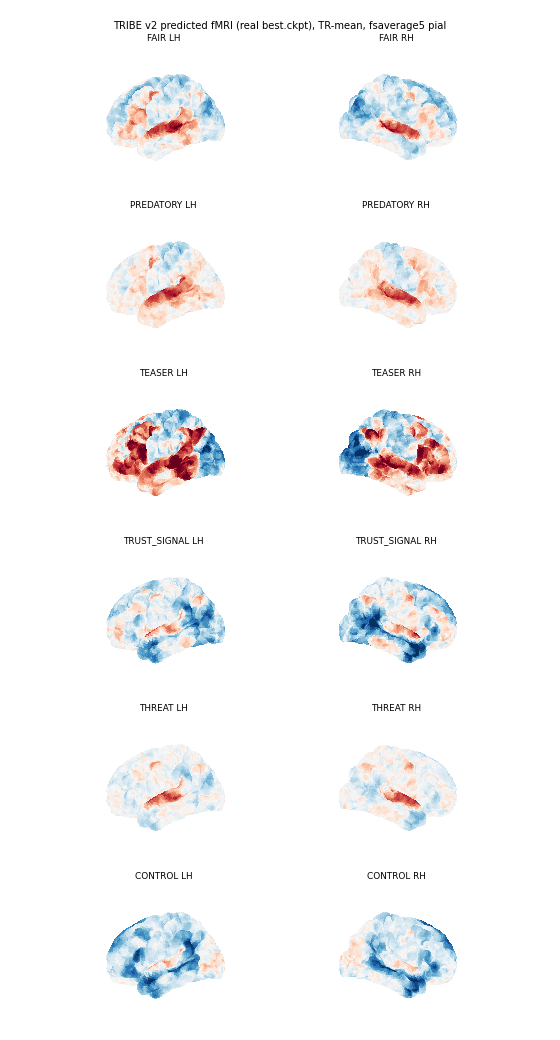
\includegraphics[width=0.49\textwidth]{figures/fig1_surface_means.png}\hfill
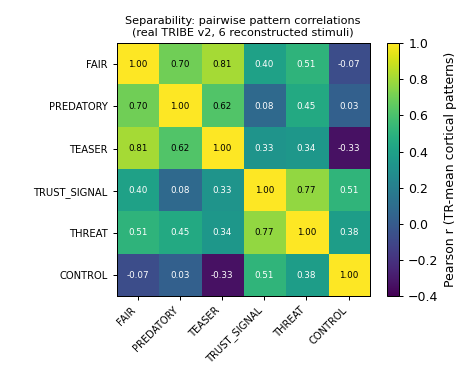
\includegraphics[width=0.49\textwidth]{figures/fig5_similarity_matrix.png}
\caption{TRIBE v2 submission re-run (official Python reference; deterministic; \S{}5.2; \textbf{reconstructed} offer-category stimuli with uniform word timing, the verbatim \S{}M texts bundled with the Supporting Document (deposit pending)). Left: TR-mean predicted cortical response per stimulus (six categories, lateral views on the real fsaverage5 pial mesh). Right: pairwise Pearson similarity of the TR-mean patterns --- every pair distinct ($r$ from $-0.33$ to $+0.81$, all cleanly below 1.0), a qualitative reproduction of the separability claim; values sit below the verbatim-stimulus battery's 0.82--0.99 because the stimuli are reconstructions, not the originals.}
\label{fig:tribe-sep}
\end{figure*}

\begin{figure*}[!tp]
\centering
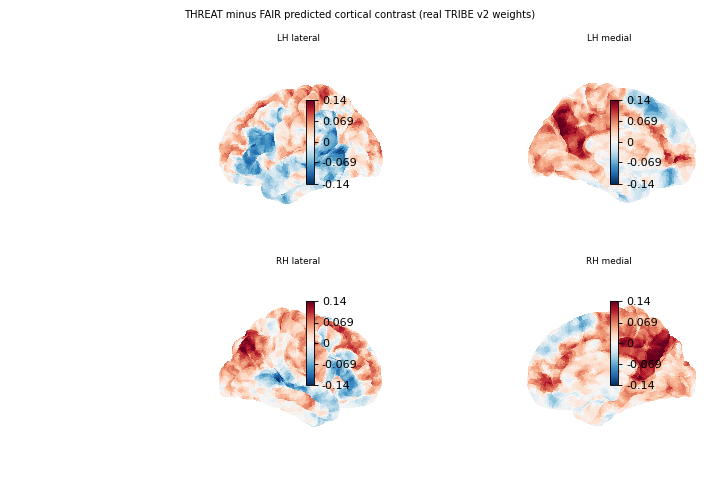
\includegraphics[width=0.49\textwidth]{figures/fig2_contrast_threat_minus_fair.png}\hfill
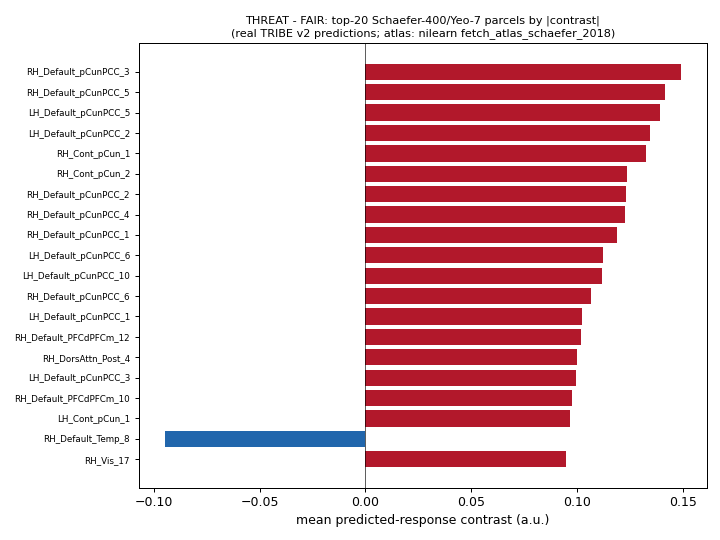
\includegraphics[width=0.49\textwidth]{figures/fig3_parcel_bars_threat_minus_fair.png}
\caption{Submission re-run, THREAT$-$FAIR vertex-wise contrast (reconstructed stimuli; descriptive contrast, not an inferential statistic). Left: contrast rendered on fsaverage5 pial surfaces (4 views). Right: top-20 Schaefer-400 parcels by $|$contrast$|$ --- 16 of 20 are Default-mode (Default\_pCunPCC dominant) or Control network parcels, the same network family as the main-text localization, with exact parcels differing across the different texts.}
\label{fig:tribe-contrast}
\end{figure*}

\begin{figure*}[!tp]
\centering
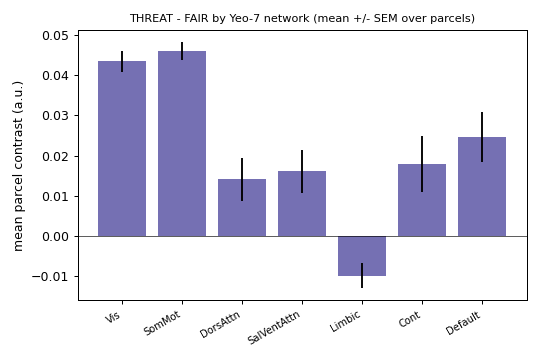
\includegraphics[width=0.49\textwidth]{figures/fig4_yeo7_network_contrast.png}\hfill
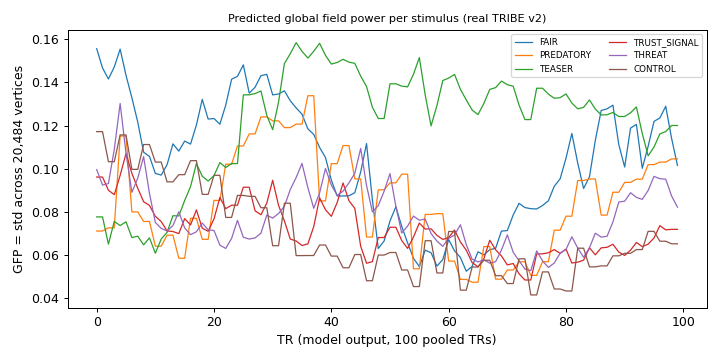
\includegraphics[width=0.49\textwidth]{figures/fig6_gfp_timeseries.png}
\caption{Submission re-run, network-level summary and dynamics. Left: Yeo-7 network means $\pm$ SEM of the THREAT$-$FAIR contrast. Right: global field power (vertex-wise SD) over the 100 predicted TRs per stimulus (deterministic; \S{}5.2).}
\label{fig:tribe-net}
\end{figure*}

\begin{figure*}[!tp]
\centering
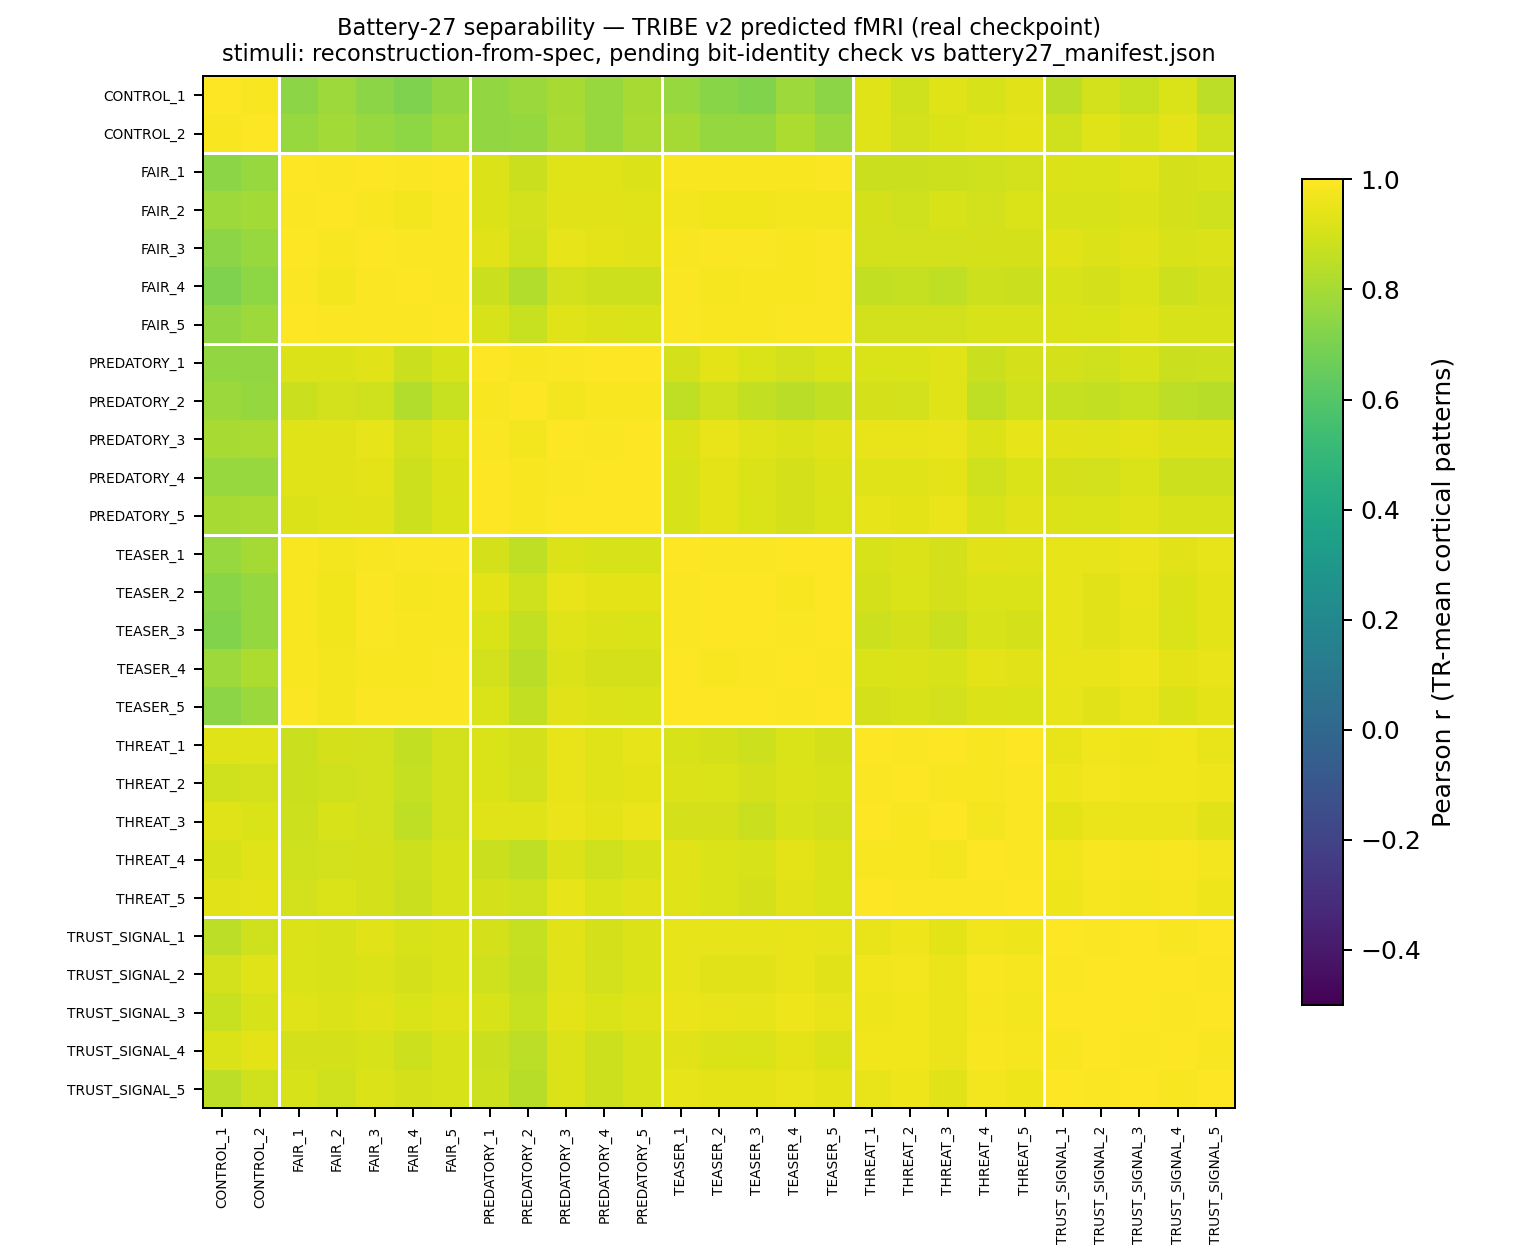
\includegraphics[width=0.92\textwidth]{figures/fig_n1_separability_matrix.png}
\caption{Extended battery, N.1 separability (\S{}5.2; \textbf{reconstruction-from-spec battery, pending bit-identity against \texttt{battery27\_manifest.json}}): $27 \times 27$ pairwise Pearson correlation of TR-mean predicted cortical patterns from the canonical pipeline (no-BOS LLaMA-3.2-3B, layers 17 \& 24, 100-TR resample, real TRIBE v2). Within-category mean $r = 0.991$, between-category $r = 0.908$, minimum pair $r = 0.708$; all 351 pairs distinct (max off-diagonal 0.998 $< 1$). Within-category values are inflated by the reconstruction's one-template-per-category lexicon --- a reconstruction property, not a model property (deterministic; \S{}5.2).}
\label{fig:n1sep}
\end{figure*}

\begin{figure*}[!tp]
\centering
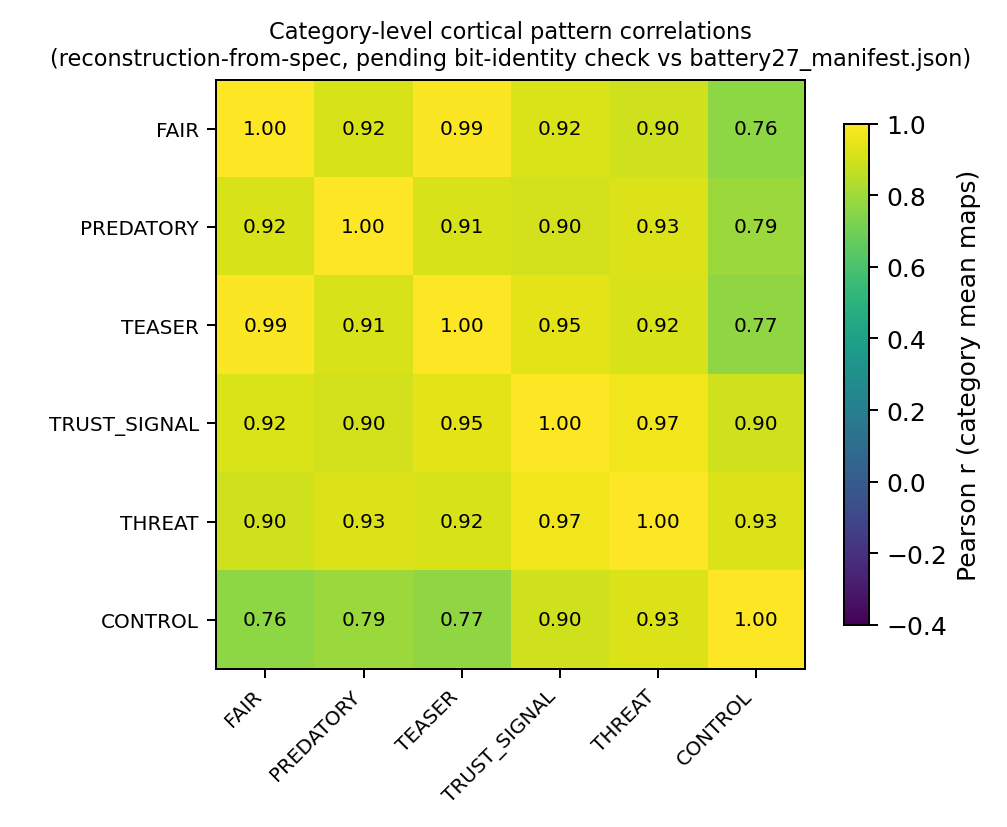
\includegraphics[width=0.92\textwidth]{figures/fig_n1_category_contrast_matrix.png}
\caption{Extended battery, N.1 category structure (same reconstruction-from-spec label as Figure~\ref{fig:n1sep}): $6 \times 6$ matrix of category mean-map correlations. Every offer category is distinct at category level; category contrasts vs.\ CONTROL: PREDATORY largest (mean $|\Delta|$ 0.070, max 0.349), then FAIR (0.053), TEASER (0.050), TRUST\_SIGNAL (0.030), THREAT (0.026).}
\label{fig:n1catmat}
\end{figure*}

\begin{figure*}[!tp]
\centering

\includegraphics[width=0.92\textwidth]{figures/fig_n1_category_contrasts.png}
\caption{Extended battery, N.1 vertex-wise contrasts (same reconstruction-from-spec label as Figure~\ref{fig:n1sep}): per-category $-$ CONTROL predicted-contrast maps rendered on the real fsaverage5 pial surface. Descriptive contrasts, not inferential statistics (descriptive contrasts only, \S{}5.2); evaluative/attentional networks dominate, consistent with the core-battery localization.}
\label{fig:n1contrasts}
\end{figure*}

\begin{figure*}[!tp]
\centering
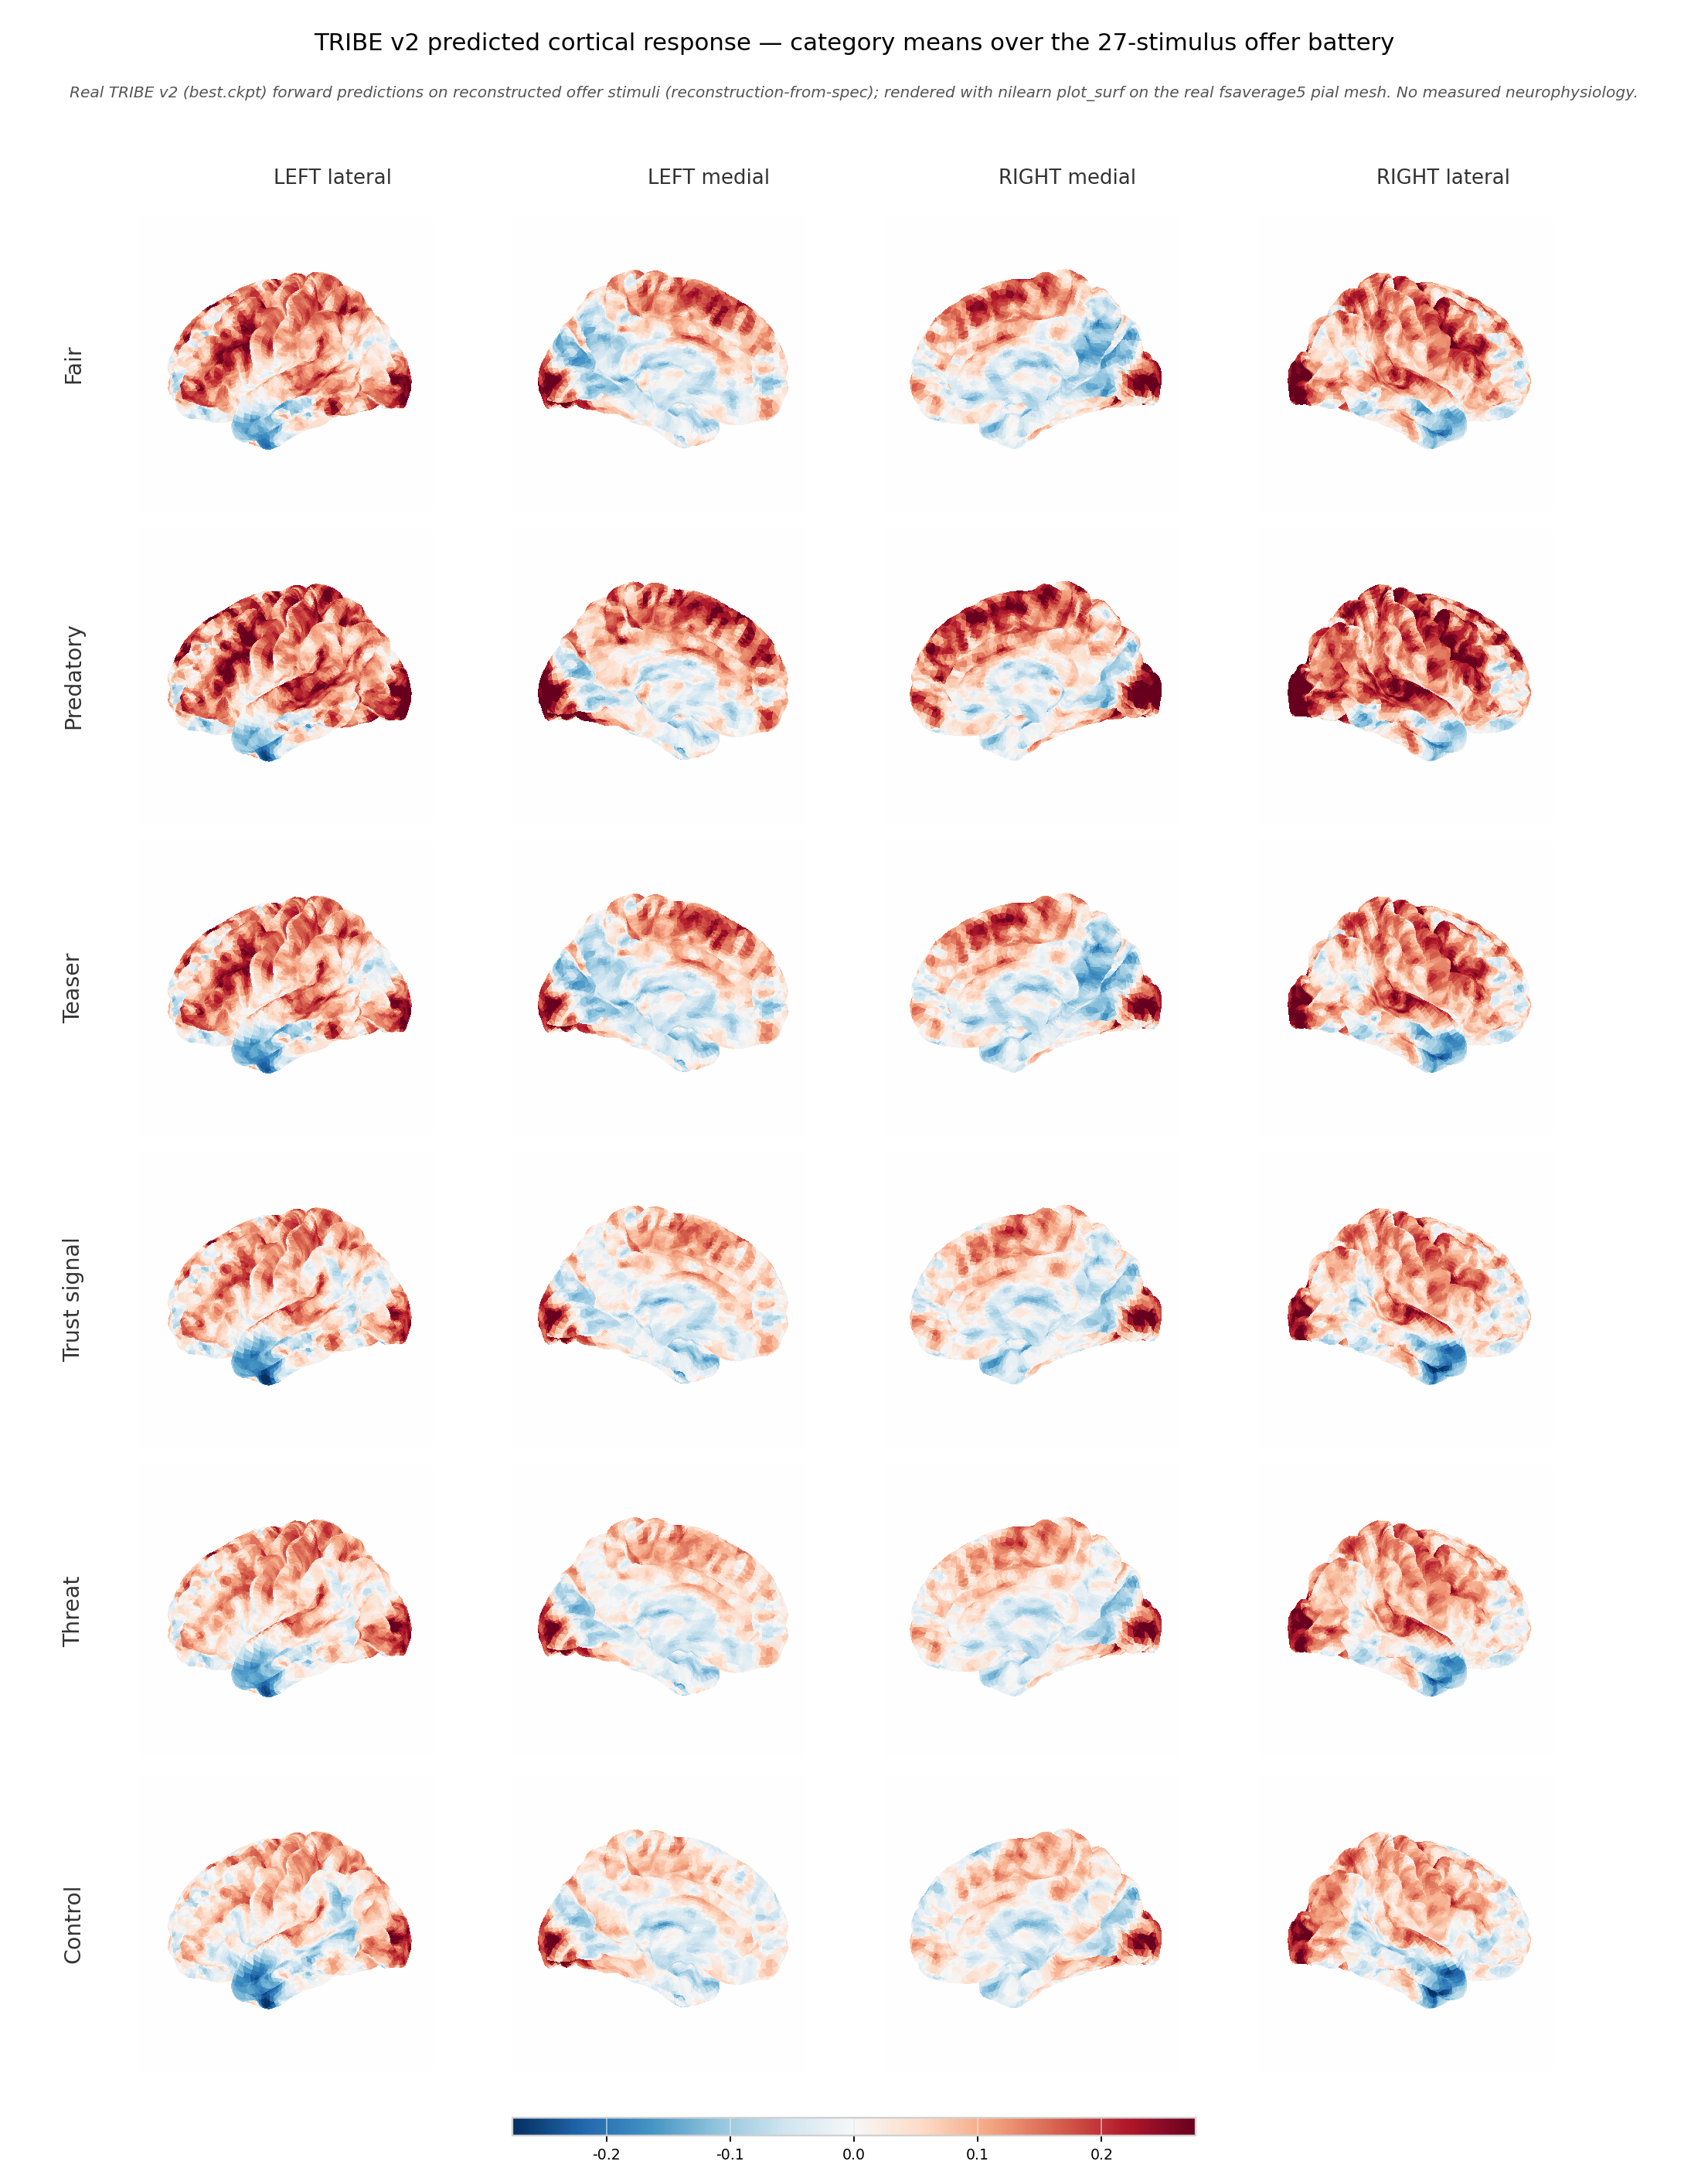
\includegraphics[width=0.98\textwidth]{figures/viz1a_category_mean_maps.png}
\caption{Extended battery, category-mean predicted cortical maps (\S{}5.2; same reconstruction-from-spec label as Figure~\ref{fig:n1sep}). Per-category mean predicted TRIBE v2 cortical response (5 items/category; CONTROL n=2), 6 rows $\times$ 4 views (LH lateral/medial, RH medial/lateral), shared symmetric color scale ($\pm$98th percentile). \textit{Provenance:} real TRIBE v2 predictions on the reconstructed-from-spec battery --- model-predicted fMRI, no measured neurophysiology anywhere in the pipeline. Rendered with nilearn on the real fsaverage5 pial mesh (pycortex could not be built in the verification environment; labeled on the figure), in the semantic-tiling lineage of \citet{huth2016} (interactive atlas viewer: gallantlab.org/huth2016).}
\label{fig:viz-catmaps}
\end{figure*}

\begin{figure*}[!tp]
\centering
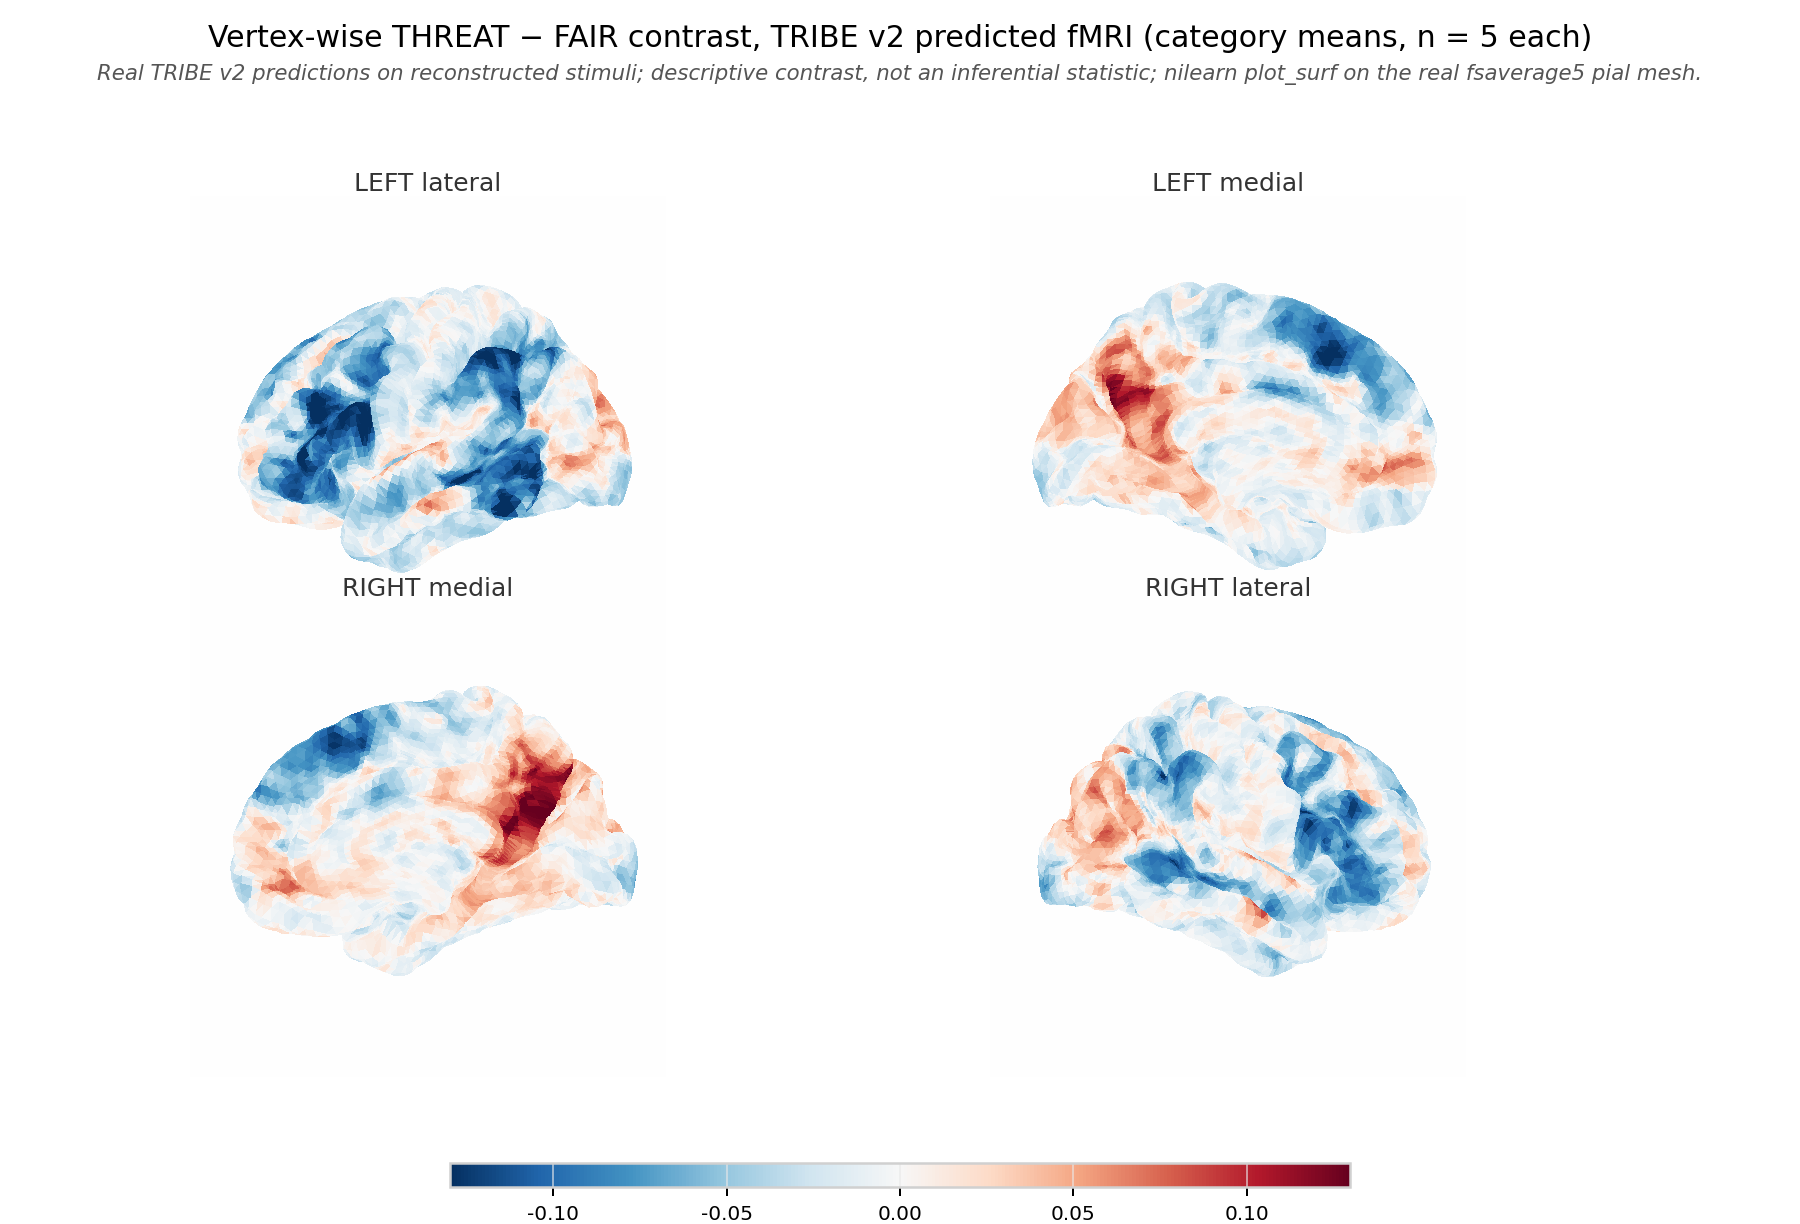
\includegraphics[width=0.98\textwidth]{figures/viz1b_contrast_threat_minus_fair.png}
\caption{Extended battery, vertex-wise THREAT$-$FAIR category-mean contrast (4 views; $\pm$99th-percentile scale; same reconstruction-from-spec provenance as Figure~\ref{fig:viz-catmaps}: real TRIBE v2 predictions on reconstructed-from-spec stimuli, rendered with nilearn on fsaverage5). \textbf{Descriptive contrast, not an inferential statistic} --- no inferential effect size is reported (\S{}5.2: no valid effect-size denominator exists for a deterministic model).}
\label{fig:viz-contrast}
\end{figure*}

\begin{figure*}[!tp]
\centering
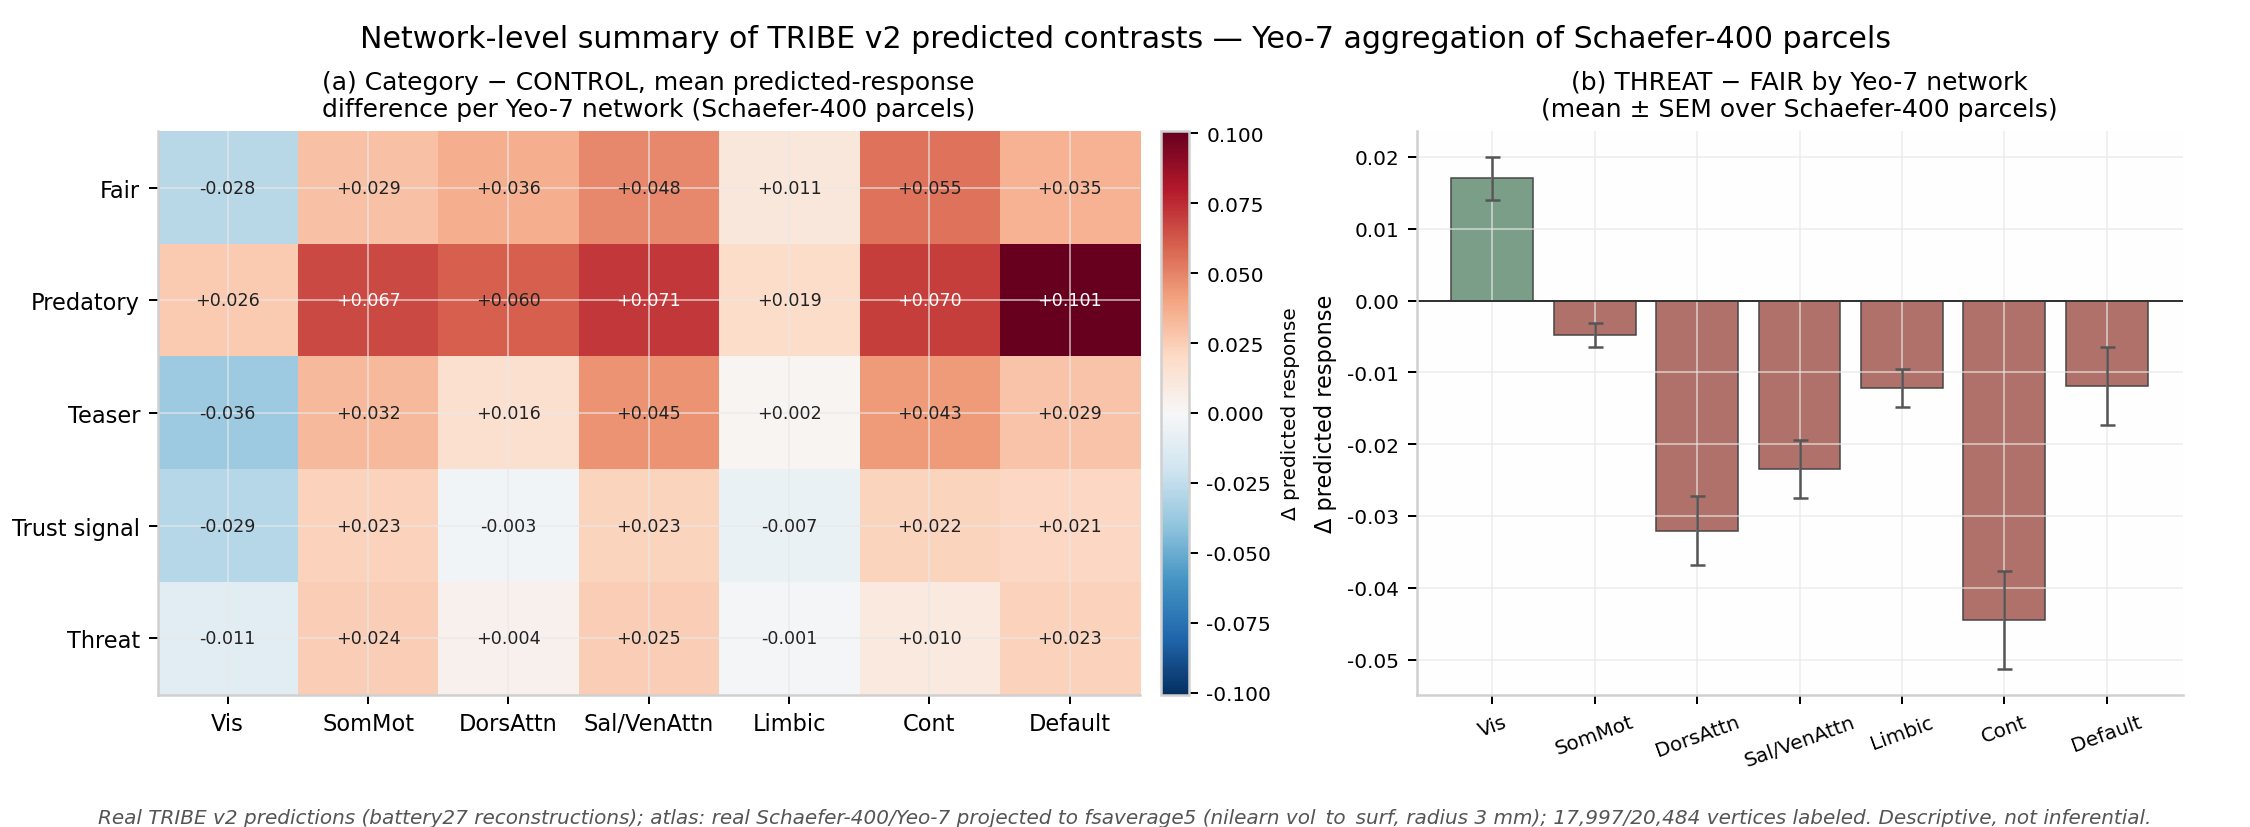
\includegraphics[width=0.98\textwidth]{figures/viz1c_yeo7_network_summary.png}
\caption{Extended battery, network-level summary (same provenance as Figure~\ref{fig:viz-catmaps}). Real Schaefer-400/Yeo-7 atlas projected to fsaverage5 (17{,}997/20{,}484 vertices labeled). (a) $5 \times 7$ heatmap of category$-$CONTROL mean $\Delta$ per Yeo-7 network (values annotated). (b) THREAT$-$FAIR network bars, mean $\pm$ SEM over parcels: Cont (largest negative, $-0.045$), DorsAttn ($-0.032$), SalVentAttn ($-0.024$) negative; Vis positive ($+0.017$) --- consistent with \S{}5.2's control/dorsal-attention/default-mode localization, reported descriptively.}
\label{fig:viz-yeo7}
\end{figure*}

\begin{figure*}[!tp]
\centering
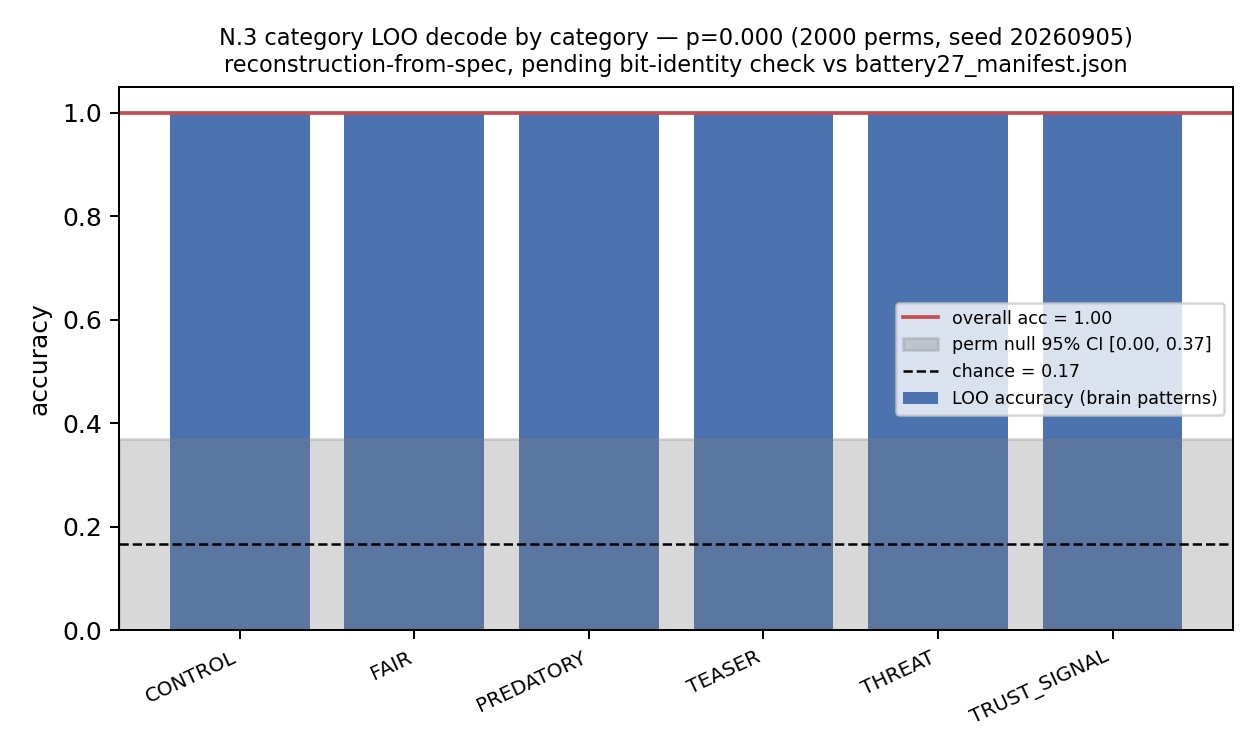
\includegraphics[width=0.92\textwidth]{figures/fig_n3_decode_bars.png}
\caption{Extended battery, N.3 Gallant-style decode with the \textbf{real} Huth-lab english1000 985-dimensional semantic model (OpenNeuro ds003020 derivatives; same matrix as Huth et al.\ 2016) (same reconstruction-from-spec label as Figure~\ref{fig:n1sep}; 2,000 permutations per null, seed 20260905, leave-8-out folds). Ridge encoding generalizes (mean vertex $r = 0.181$, $p = 0.0005$, resolution-limited at 2{,}000 permutations); exact stimulus retrieval is NULL (top-1 0.037, $p = 1.0$) and Procrustes alignment is NULL ($r = -0.058$, $p = 0.769$) --- matching the original battery's reported null pattern (reference only). Category leave-one-out decode is perfect (1.000, $p = 0.0005$) but is driven by the reconstruction's templatic within-category lexicon --- the semantic-only control decodes at 1.000 too --- and is explicitly NOT comparable to the original battery's 0.40.}
\label{fig:n3decode}
\end{figure*}

\begin{figure*}[!tp]
\centering
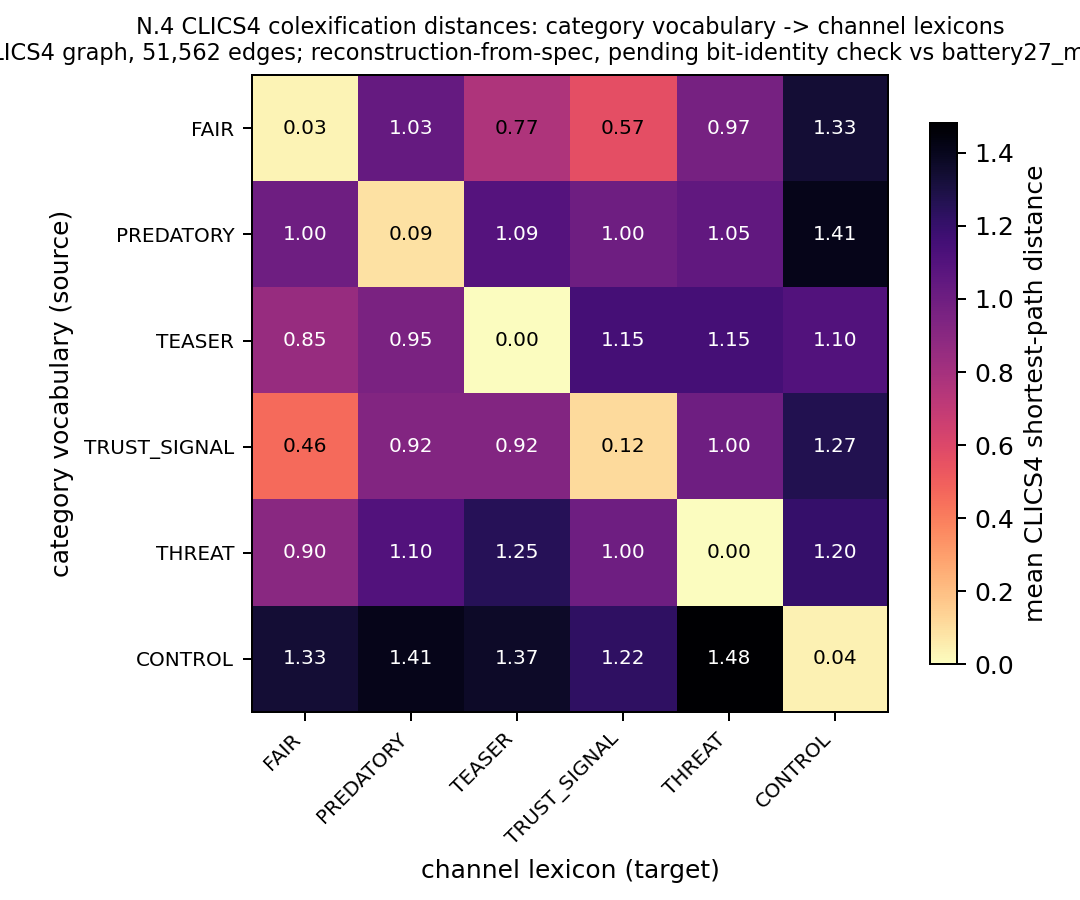
\includegraphics[width=0.92\textwidth]{figures/fig_n4_clics_heatmap.png}
\caption{Extended battery, N.4 CLICS4 overlap (same reconstruction-from-spec label as Figure~\ref{fig:n1sep}; real CLICS4 CLDF graph, 1,725 nodes / 51,562 edges): category-vocabulary $\to$ channel-lexicon mean shortest-path distances. 114 of 196 content words mapped to Concepticon nodes (tiered matching fully logged: 52 exact gloss, 19 morphological, 43 via a documented synonym table; 82 unmapped, mostly finance jargon with no Concepticon gloss). Every category sits at distance $\approx 0$ from its own channel lexicon and $\geq 0.5$ from all others; CONTROL is the farthest from every offer category (1.08--1.48). Channel lexicons are battery-derived (the paper's channel-concept lists are in the Supporting Document (deposited at OSF)) and are labeled as such; the diagonal is by construction (battery-derived lexicons) --- only off-diagonal distances carry content.}
\label{fig:n4clics}
\end{figure*}

\begin{figure*}[!tp]
\centering
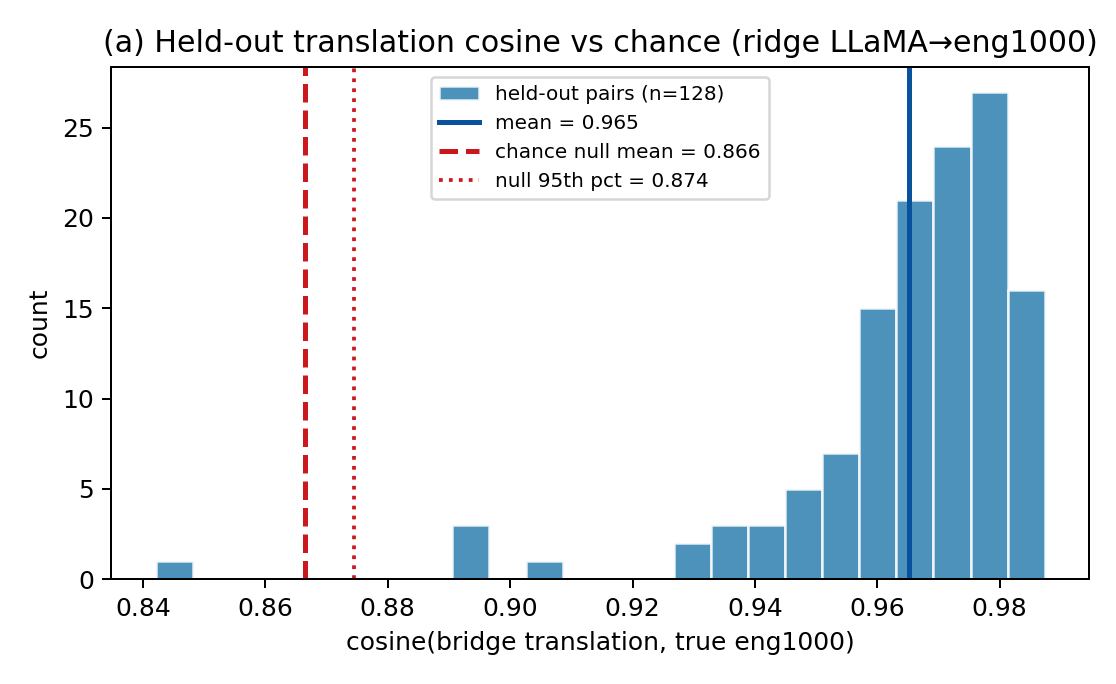
\includegraphics[width=0.92\textwidth]{figures/bridge_a_cosine_dist.png}
\caption{Supervised LLaMA $\to$ eng1000 ridge bridge (\S{}5.2) --- held-out cosine, reported only against its null ($N = 640$ paired real NQ-corpus texts, 64-token chunks, eng1000 coverage $\geq 0.5$; 512 train / 128 held-out; seed 42; ridge $\alpha = 3162$ by 5-fold CV). Held-out paired mean cosine 0.965 vs.\ random-pairing null mean 0.866 (null p95 0.874); permutation $p = 0.0005$ (2{,}000 reps). The null is high because eng1000 is anisotropic --- the signal is paired $\gg$ null, not the absolute cosine value.}
\label{fig:bridge-cos}
\end{figure*}

\begin{figure*}[!tp]
\centering
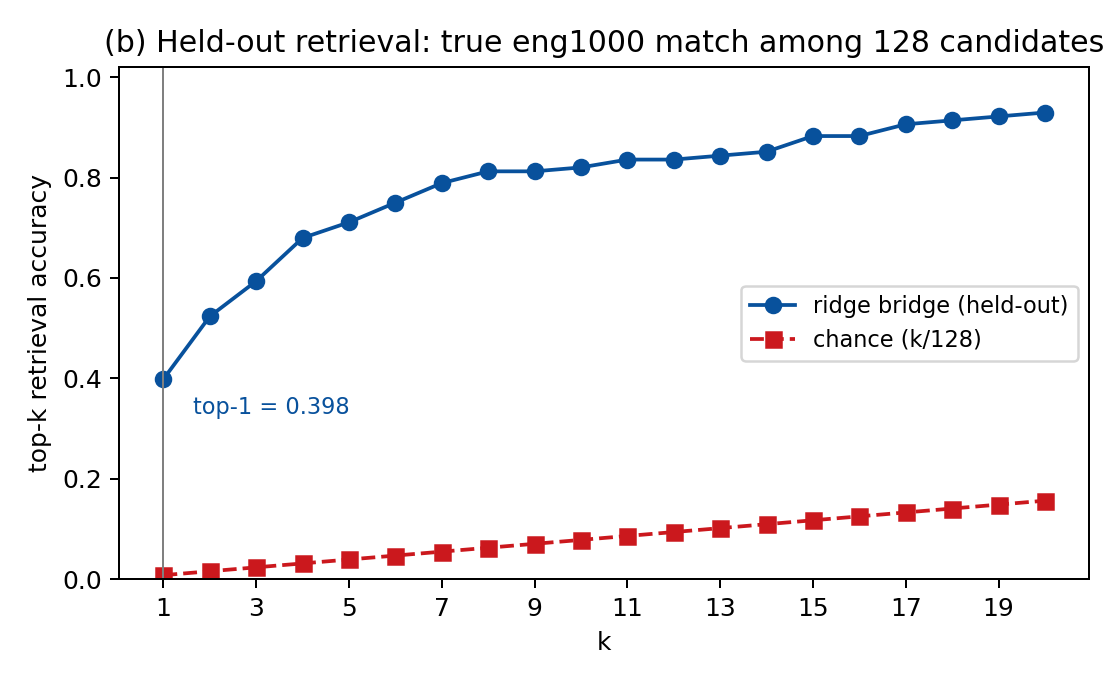
\includegraphics[width=0.92\textwidth]{figures/bridge_b_topk.png}
\caption{Bridge retrieval on the 128 held-out pairs (\S{}5.2). Top-1 0.398 vs.\ chance 0.0078 (51$\times$), top-5 0.594 vs.\ 0.039; mean rank 6.9 vs.\ chance 64.5. A rectangular orthogonal Procrustes comparison is comparable on retrieval rank only. $N = 640$ is a CPU-feasibility scale; the full-scale recipe is documented in the GCP runbook.}
\label{fig:bridge-topk}
\end{figure*}

\begin{figure*}[!tp]
\centering
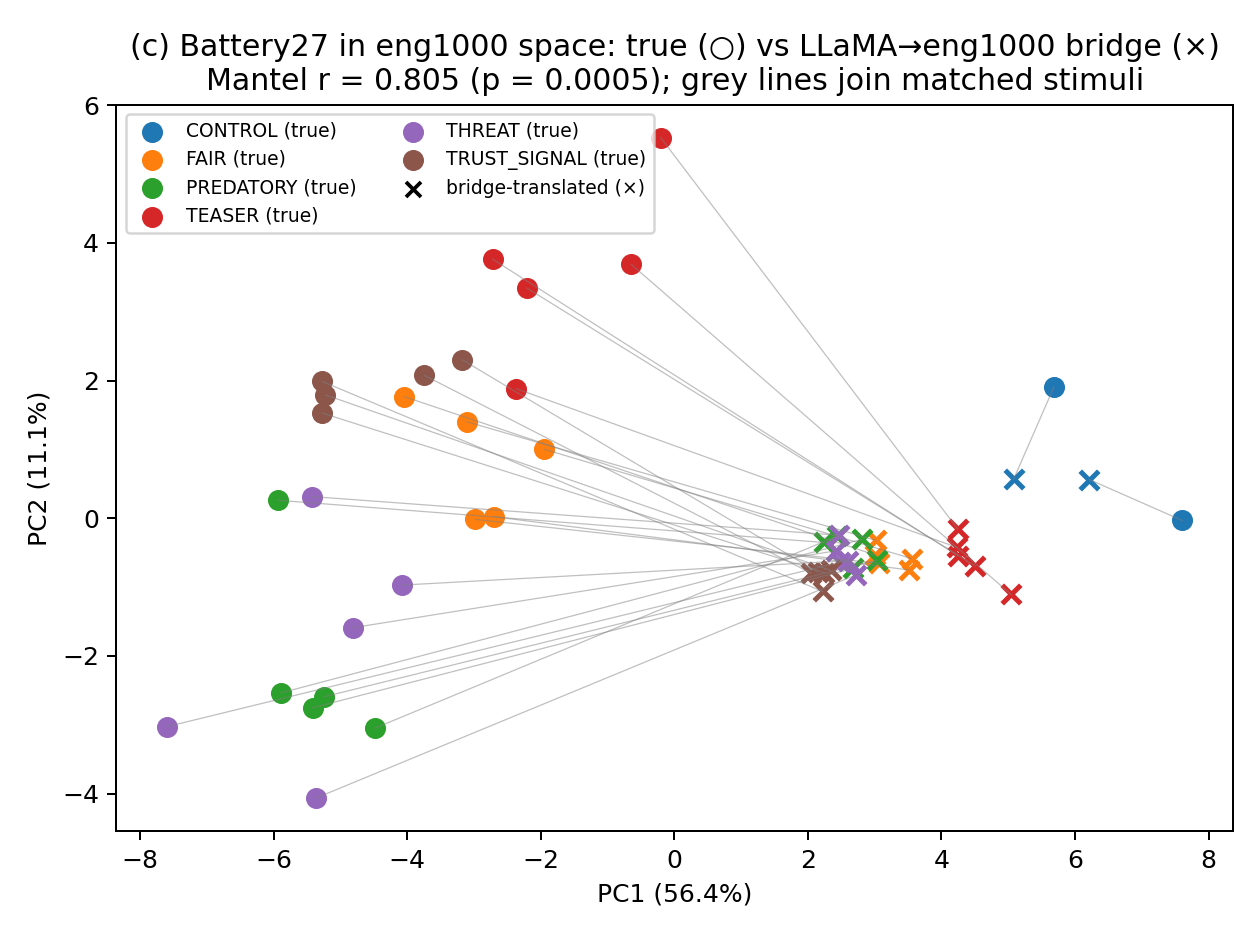
\includegraphics[width=0.92\textwidth]{figures/bridge_c_pca_battery.png}
\caption{Battery27 downstream in eng1000 space via the bridge (same \textbf{reconstruction-from-spec} label as Figure~\ref{fig:n1sep}). PCA of true eng1000 features vs.\ LLaMA features translated through the ridge map: translated-vs-true per-item cosine 0.813 (tight null 0.791, $p = 0.0005$); RDM Mantel $r = 0.805$, $p = 0.0005$ (raw un-translated LLaMA RDM: $r = 0.362$ --- the bridge doubles the geometry match); category LOO decode 1.00. The ridge's regression-to-mean shrinkage toward the centroid is visible, and exact-item retrieval among the 27 is at chance because same-category items are near-duplicates in true eng1000 space itself; category-level geometry --- what the pipeline consumes --- is preserved.}
\label{fig:bridge-pca}
\end{figure*}

\begin{figure*}[!tp]
\centering
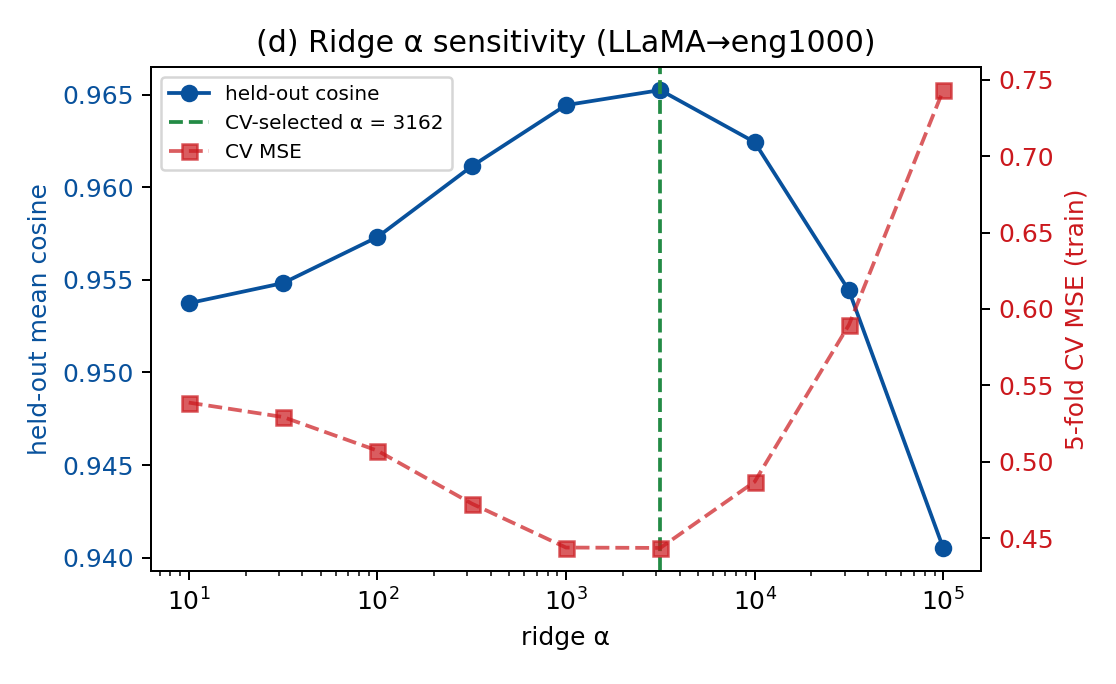
\includegraphics[width=0.92\textwidth]{figures/bridge_d_alpha.png}
\caption{Bridge regularization selection (\S{}5.2). 5-fold CV MSE over $\alpha \in \{10^{1}\dots10^{5}\}$ on the 512 training pairs; selected $\alpha = 3162$ for LLaMA $\to$ eng1000, refit on the full training set.}
\label{fig:bridge-alpha}
\end{figure*}

\begin{figure*}[!tp]
\centering
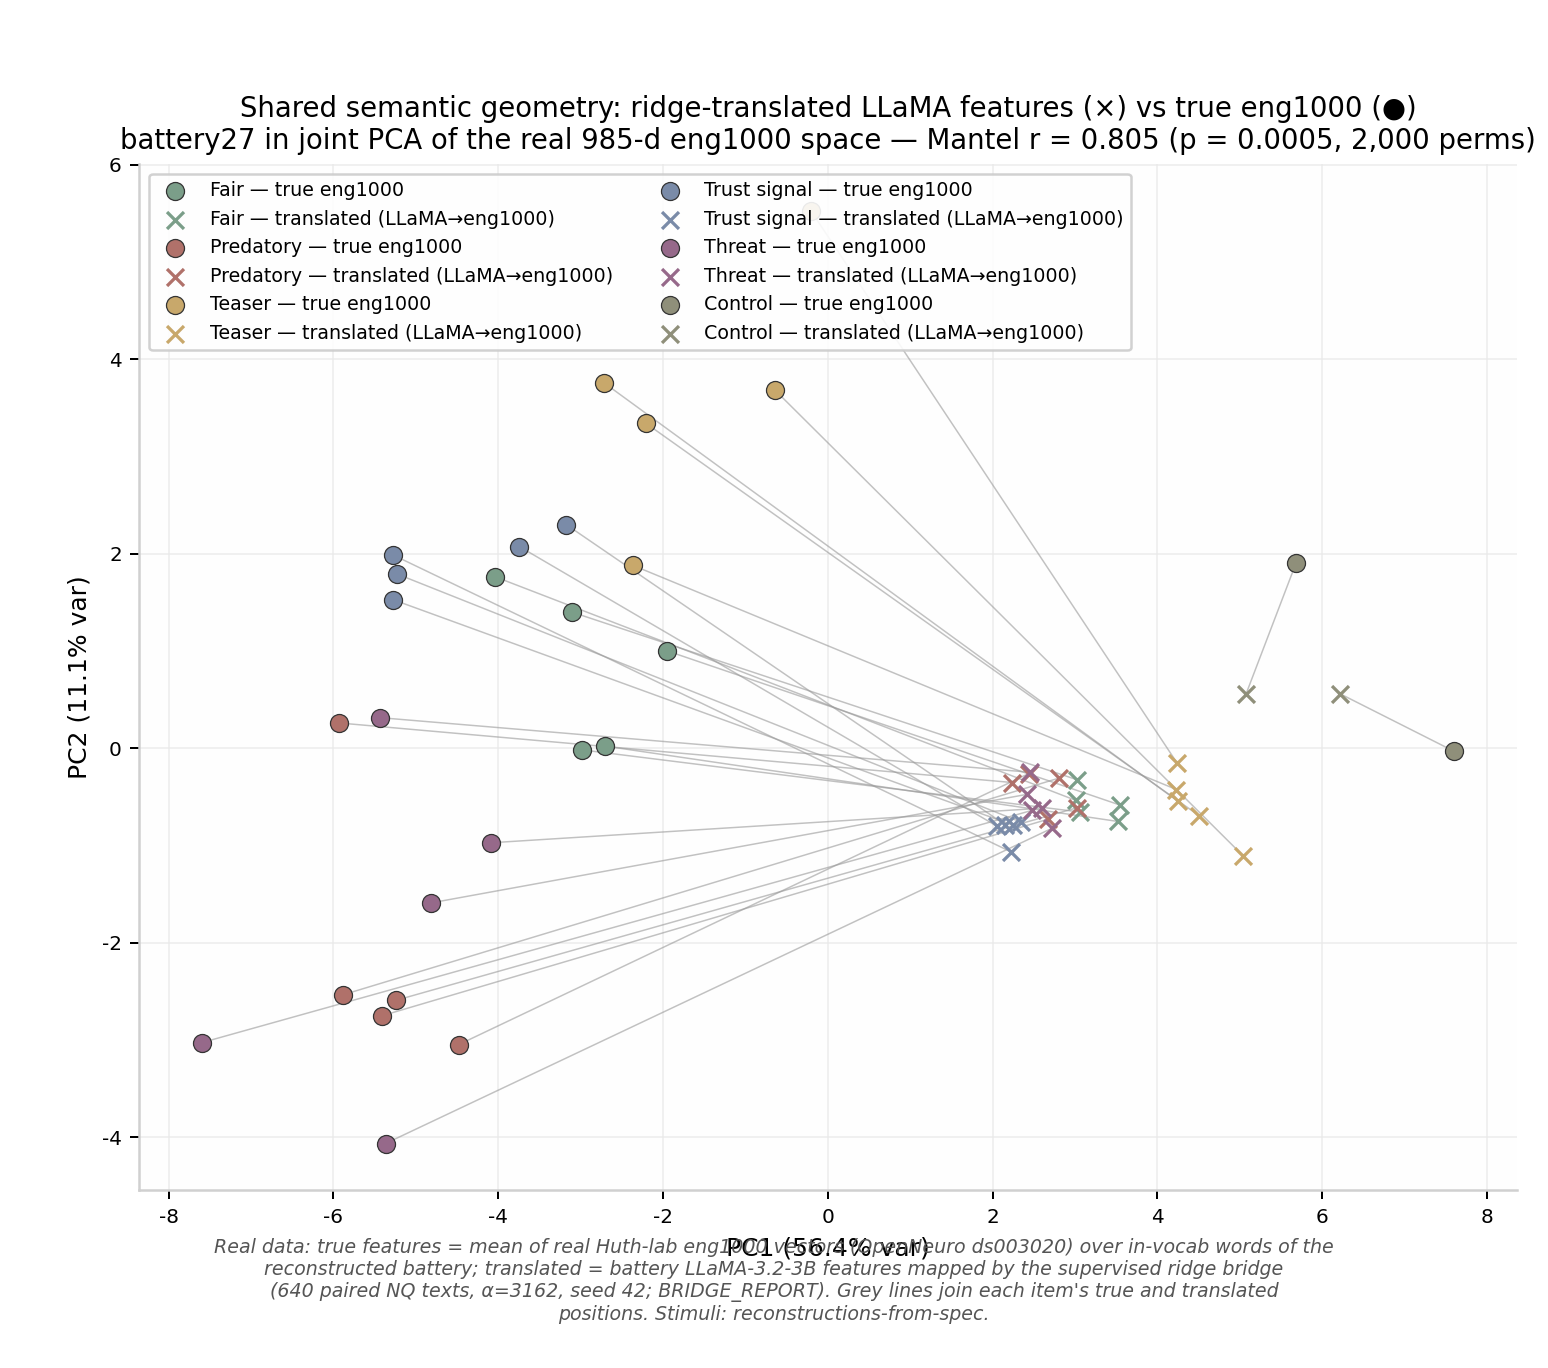
\includegraphics[width=0.49\textwidth]{figures/viz2a_bridge_geometry_pca.png}\hfill
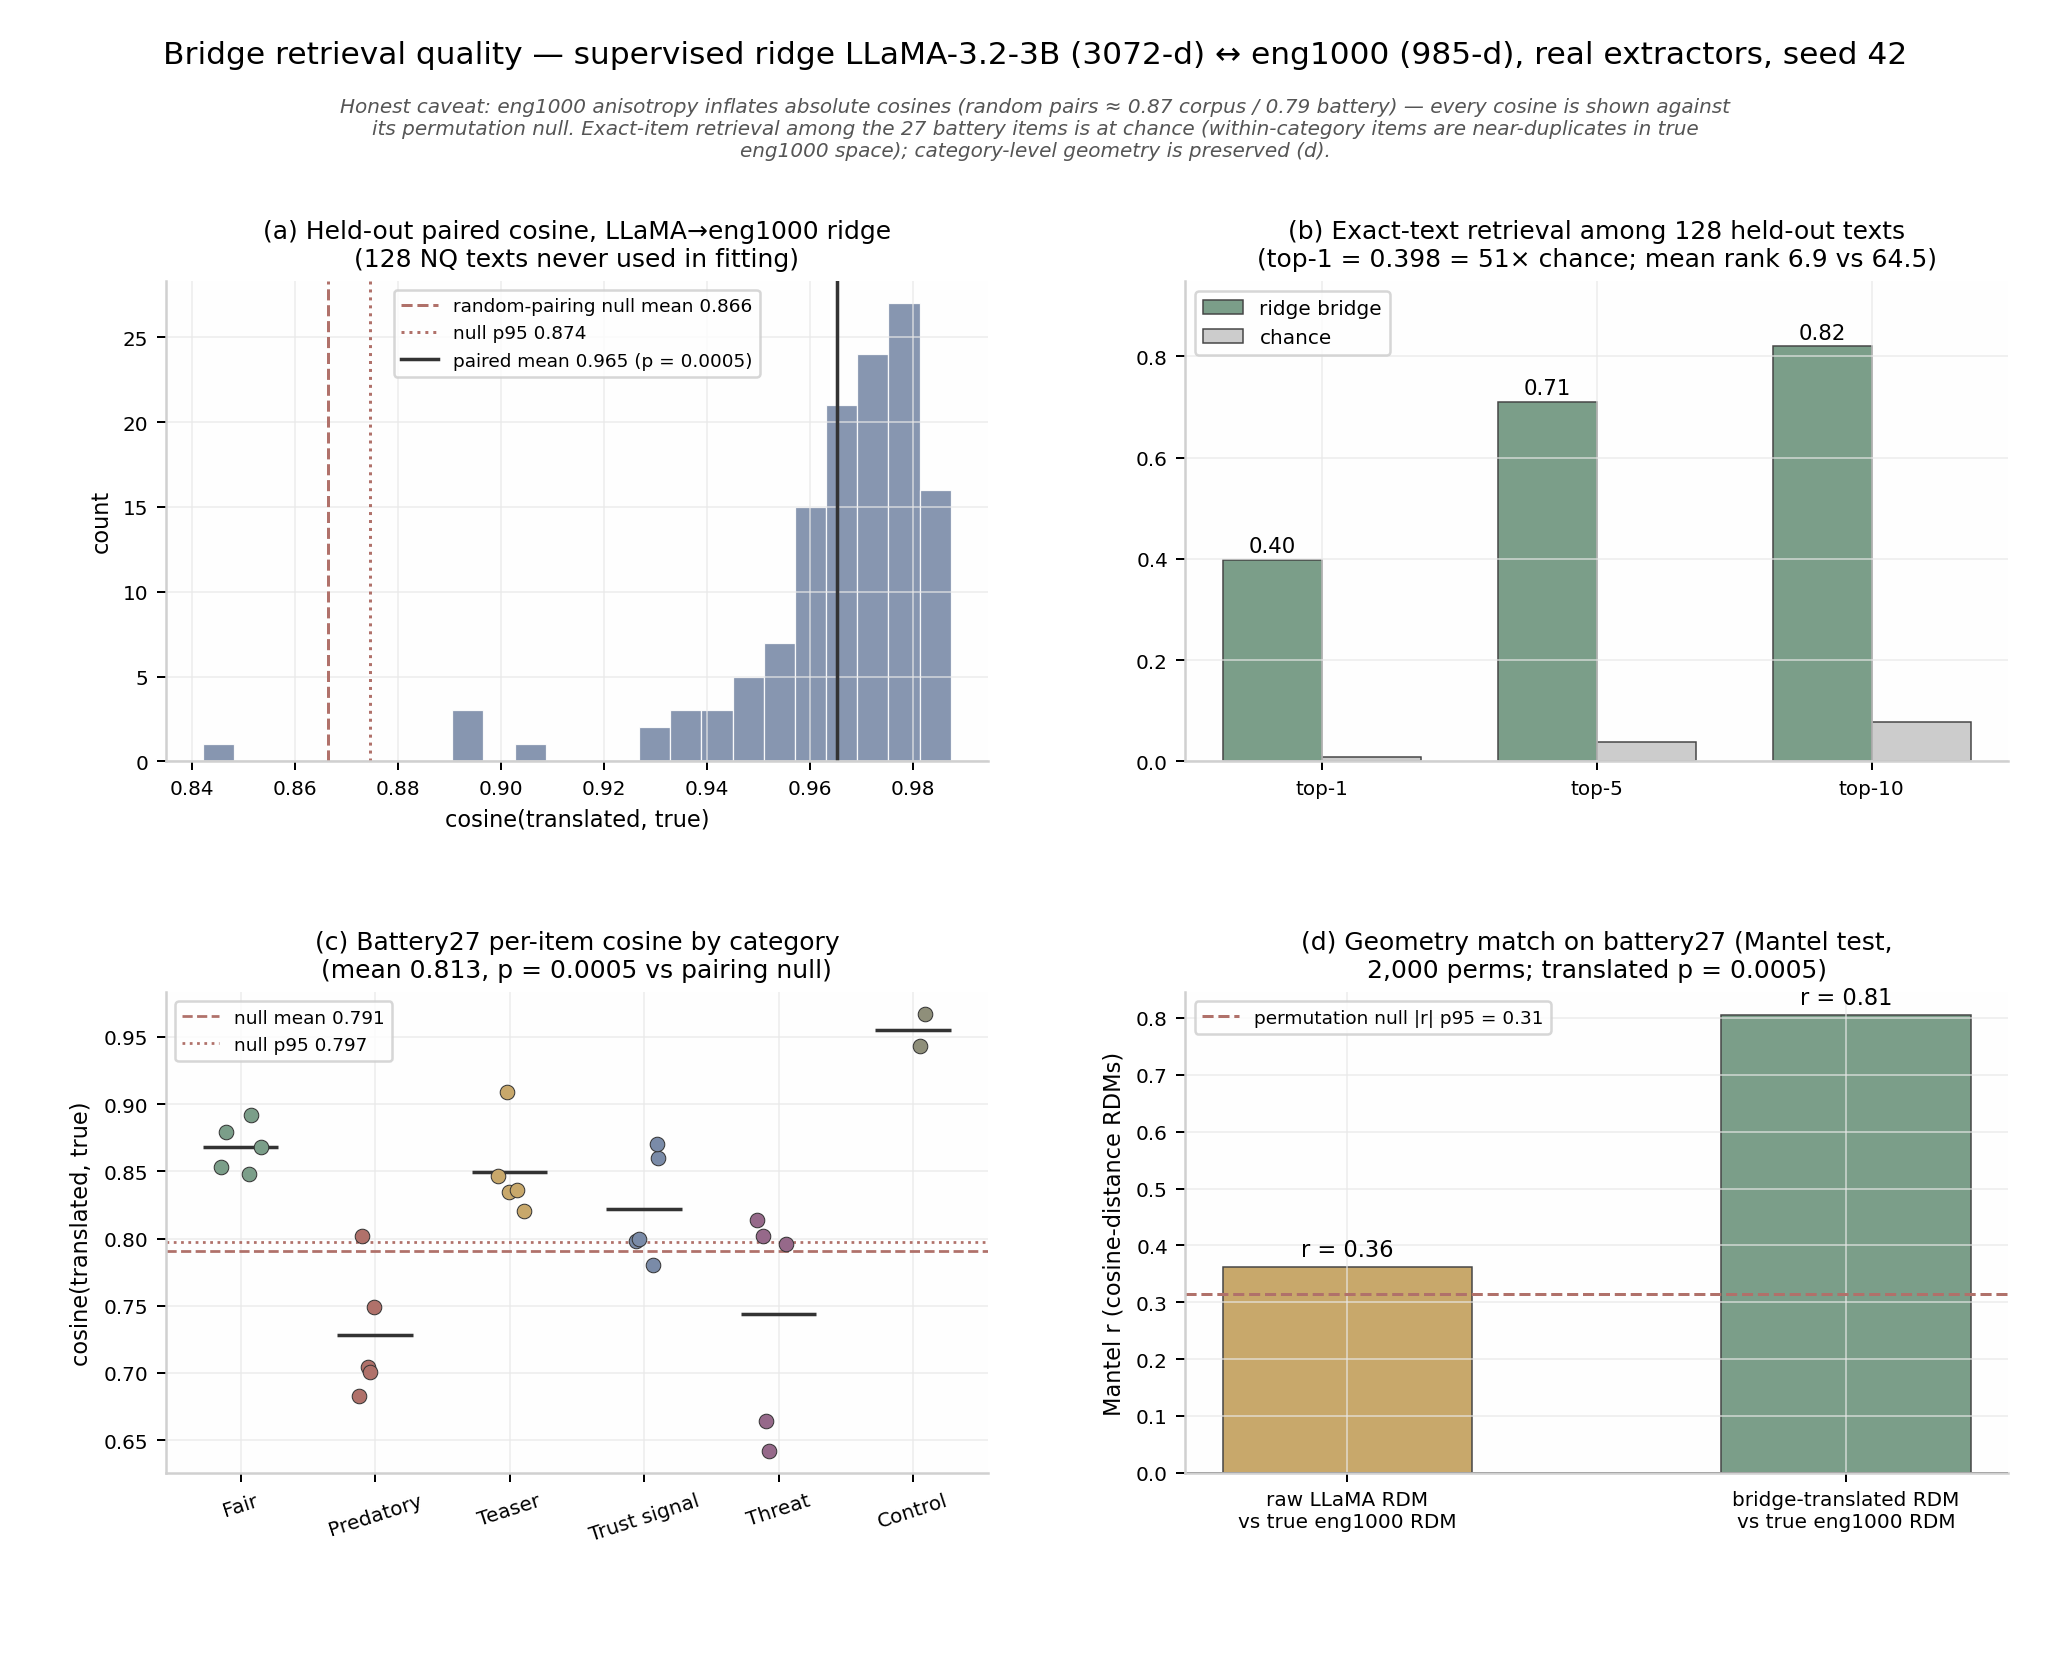
\includegraphics[width=0.49\textwidth]{figures/viz2b_bridge_retrieval_summary.png}
\caption{Bridge shared-latent geometry and retrieval summary (\S{}5.2; real bridge results, seed 42; same reconstruction-from-spec battery label as Figure~\ref{fig:n1sep}). Left: joint PCA (fit on the 54 stacked vectors) of true eng1000 battery features (dots) vs.\ ridge-translated LLaMA features (crosses), colored by battery category, with grey pairing lines; header carries the Mantel geometry match ($r = 0.805$, $p = 0.0005$). The translated cloud shrinks toward the centroid (ridge regression-to-mean) while category structure is preserved --- exactly what the Mantel number quantifies. The true battery features were recomputed from the real \texttt{english1000sm.hf5} (OpenNeuro ds003020 snapshot) with the exact pipeline code path; recomputed per-item translated-vs-true cosines match the archived bridge results to $\max|\Delta| = 1.2\times10^{-9}$ --- a functional bit-check of the whole chain. Right: retrieval-quality panel --- held-out cosine histogram (128 NQ pairs, mean 0.965) against the random-pairing null (mean 0.866 / p95 0.874; the anisotropy caveat is stated on the figure), top-$k$ retrieval vs.\ chance, battery27 per-item cosine by category vs.\ the pairing null, and the Mantel geometry match (bridge 0.805 vs.\ raw-LLaMA 0.362 vs.\ null $|r|$ p95 0.315).}
\label{fig:viz-bridge}
\end{figure*}

\textbf{Battery extension.} The stimulus set was expanded from 6 to 27 fabricated texts — five offers per category at five principal amounts, plus two non-financial controls — and the same real-weights pipeline re-run end-to-end (full protocol and statistics: Supporting Document \S{}N). All 27 stimulus texts carry the label \textbf{``reconstruction-from-spec, pending bit-identity check against \texttt{simulations/battery27\_manifest.json}''}: item 1 of each category is a verbatim quote from the Master Reproduction Manifest; items 2--5 (+ CONTROL\_2) were written to the manifest's stated design intents. Findings:

\begin{itemize}

\item \textbf{N.1 (pipeline and separability; Figures~\ref{fig:n1sep}--\ref{fig:n1contrasts}; category-mean surfaces, THREAT$-$FAIR contrast, and network summary: Figures~\ref{fig:viz-catmaps}--\ref{fig:viz-yeo7}).} The canonical per-stimulus chain --- no-BOS LLaMA-3.2-3B tokenization, hidden states at layers 17 \& 24 (manifest stand-ins for the group-mean ranges), uniform token resample to 100 TRs, real TRIBE v2 forward --- ran on all 27/27 stimuli. Determinism replicates bit-exactly ($\max|\Delta| = 0.0$ on a full independent re-run). Separability holds: within-category mean $r = 0.991$, between-category $r = 0.908$, minimum pair $r = 0.708$, all 351 pairs distinct (max off-diagonal $0.998 < 1$). Caveat: within-category correlations are higher than round M's six-stimulus set because the reconstructed battery uses one template per category --- a reconstruction property, not a model property. Category contrasts vs.\ CONTROL: PREDATORY largest (mean $|\Delta|$ 0.070, max 0.349), then FAIR (0.053), TEASER (0.050), TRUST\_SIGNAL (0.030), THREAT (0.026).
- Localization replicates at category level (n = 5 offers each): category-mean contrasts again peak in control, dorsal-attention, and default-mode networks (THREAT-FAIR top parcels LH Cont\_Par\_4/5/6, LH DorsAttn\_Post\_9; TRUST\_SIGNAL-PREDATORY top RH Cont\_PFCl\_12/14, RH Default\_pCunPCC\_9). Reported as raw vertex-wise contrast magnitudes; normalized effect sizes against a deterministic model's temporal variability are not interpretable and are omitted (correction as above). Vertex-wise contrast maps rendered on the real fsaverage5 pial surface are included as Figure~\ref{fig:n1contrasts}.
- \textbf{N.3 Gallant-style decoding, now against the real semantic model (Figure~\ref{fig:n3decode}; Supporting Document \S{}N.3).} The semantic features are means of the real Huth-lab english1000 985-dimensional vectors (OpenNeuro ds003020 derivatives; the same matrix as Huth et al.\ 2016 --- not a substitute), coverage 0.78--0.97 of in-vocab words per stimulus; ridge $\alpha = 10^{3}$, 2,000 permutations per null, leave-8-out folds, seed 20260905. Voxelwise ridge encoding generalizes (mean vertex $r = 0.181$, $p = 0.0005$ --- resolution-limited: the minimum achievable value at 2{,}000 permutations, i.e., $p \leq 0.0005$); exact stimulus retrieval is a NULL (top-1 0.037 $= 1/27$, $p = 1.0$) and unsupervised Procrustes alignment is a NULL ($r = -0.058$, $p = 0.769$) --- reproducing the \emph{pattern} of the original battery's reported nulls (reference only). Category leave-one-out decode is perfect (1.000, $p = 0.0005$; permutation-null 95\% CI [0.00, 0.37]) but is driven by the reconstruction's within-category lexical homogeneity --- the semantic-only control also decodes at 1.000, so the brain patterns inherit a trivially separable input --- and it is \textbf{explicitly not comparable to the original battery's 0.40}, which implies the true battery had much higher within-category lexical diversity.
- \textbf{vec2vec bridge (unblocked at instrument level; geometry and retrieval rendered in Figure~\ref{fig:viz-bridge}).} The released vec2vec v1.0.0 pretrained translators \citep{jha2025} were downloaded and run on CPU (state-dict strict load, 0 missing / 0 unexpected keys; the \texttt{gte\_gtr} pair): embedding the 27 battery texts with the real gte-base and gtr-t5-base encoders and translating gte $\to$ gtr gives mean cosine 0.703 to the true target embedding (range 0.627--0.802) and top-1 retrieval of the correct text among 27 at \textbf{44.4\% vs.\ 3.7\% chance} (shuffle-null mean 0.0375). None of the 15 released pairs covers LLaMA hidden states or eng1000 --- but the DOCAS-specific bridge has been \textbf{built and validated as a supervised ridge map} (September 2026; full protocol in the bridge run report, runbook \S{}C.1), and that changes the training verdict: because we control both feature extractors, paired embeddings are producible, so vec2vec's unsupervised GAN --- whose only advantage is not needing paired data --- is \textbf{unnecessary for this pipeline}; vec2vec training would be required only if unpaired operation were ever needed. The bridge: 640 paired real texts (NQ corpus passages, 64-token chunks, eng1000 in-vocab coverage $\geq 0.5$), 512 train / 128 held-out, seed 42, features z-scored on train statistics, ridge $\alpha = 3162$ by 5-fold CV. Held-out, LLaMA $\to$ eng1000: mean cosine 0.965, top-1 retrieval 0.398 (\textbf{51$\times$ chance} 0.0078), top-5 0.594, mean rank 6.9 (chance 64.5), random-pairing permutation $p = 0.0005$ (2{,}000 reps); reverse eng1000 $\to$ LLaMA cosine 0.949 / top-1 0.266; a rectangular orthogonal Procrustes comparison is comparable on retrieval rank only. Downstream on the 27-stimulus battery (same reconstruction-from-spec label as Figure~\ref{fig:n1sep}): translated-vs-true eng1000 per-item cosine 0.813 (tight null 0.791, $p = 0.0005$), RDM Mantel $r = 0.805$, $p = 0.0005$ --- vs.\ $r = 0.362$ for the raw un-translated LLaMA RDM, so the bridge \textbf{doubles} the geometry match --- and category LOO decode 1.00 (Figures~\ref{fig:bridge-cos}--\ref{fig:bridge-alpha}). Caveats, carried with every number: eng1000 is anisotropic, so the random-pair cosine null is already 0.87 (corpus) / 0.79 (battery) --- cosine is reported only against its null; exact-item retrieval among the 27 is at chance because same-category items are near-duplicates in true eng1000 space itself; and $N = 640$ is CPU-feasibility scale, with the full-scale recipe documented in the GCP runbook. The gte $\to$ gtr released-pair demo above stands as the tool-level check of vec2vec itself.
- The Fisher–Rao honesty check replicates as a null: cross/within-group ratio 0.89 (round M: 0.83). Two rounds, two nulls — whole-cortex distributional distance is not a trustworthiness meter; the targeted-decoder gate stands.
- \textbf{N.4 CLICS4 overlap (Figure~\ref{fig:n4clics}; \S{}N.4).} On the real CLICS4 CLDF graph (verified at 1,725 nodes / 51,562 edges): 114 of 196 battery content words mapped to Concepticon nodes (tiered matching fully logged: 52 exact gloss, 19 morphological, 43 via an explicit documented synonym table --- e.g., payment $\to$ PAY, garnishment $\to$ SEIZE, penalty $\to$ PUNISHMENT, trust $\to$ TRUTH; 82 unmapped, mostly finance jargon with no Concepticon gloss). In the category-vocabulary $\to$ channel-lexicon mean shortest-path matrix, every category sits at distance $\approx 0$ from its own channel lexicon and $\geq 0.5$ from all others, and CONTROL is the farthest from every offer category (1.08--1.48). The channel lexicons are battery-derived --- the paper's own channel-concept lists are in the Supporting Document (deposited at OSF) --- and are labeled as such; the diagonal is by construction (battery-derived lexicons) --- only off-diagonal distances carry content.
- Cross-layer seeding: the battery's category sensitivities seed the companion protocol preprint's population model (\S{}3.6 there), making the protocol layer's heterogeneity a model-derived input — not a measured quantity, and labeled as such downstream.

\end{itemize}
An expanded 82-stimulus follow-on battery (\textbf{Sim D8}; Supporting Document \S{}S.5) — pre-registered before running — adds paraphrase controls and Spanish/Japanese arms: category geometry survives full paraphrase (LOO marginal, fails family-wise correction; the geometry correspondence survives BH only) (LOO 0.40 vs 0.20 chance, p = 0.046; EN $\times$ PAR geometry Mantel r = 0.275, p = 0.006) and the pipeline reproduces the registered English result after a from-scratch rebuild, while \textbf{the multilingual arms failed their pre-registered significance criteria} (ES p = 0.174; JA p = 0.053; EN $\times$ ES/EN $\times$ JA geometry concordance not confirmed) — a power/confound-bounded null that is reported as such and that freezes any cross-language cortical-geometry claim until a powered multilingual battery with a non-English-dominant feature extractor exists. Those nulls are instrument-compatible rather than hypothesis-falsifying: the universals literature locates what is shared at the \textit{dimensional} level (hedonic valence, physiological activation) and what varies at the item/structure level, with family-level structural variation predicted by geographic/genealogical proximity \citep{jackson2019,xu2020,karjus2021} --- dimension-level universals plus item-level family variation is exactly the EN-pass/ES-JA-fail signature for an encoder whose LLaMA-3.2 text tower is English-dominant and whose training corpus is English-language CNeuroMod movies \citep{dascoli2025} (\S{}4.6). The hypothesis is demoted pending multilingual instruments, not falsified. A pre-registered second-encoder replication attempt (\textbf{Sim D9}; Supporting Document \S{}S.6) — the \citet{tuckute2024} language-network encoder, trained on a disjoint subject pool — failed both frozen criteria (category decoding p = 0.190; TRIBE $\times$ Tuckute geometry Mantel r = 0.159, p = 0.0996); it is reported as a scope-bounded null (the second encoder measures six language-network ROIs, not the control/DMN systems where this battery's contrasts live), and the instrument claim remains single-encoder until a whole-brain second encoder replicates it. Provenance accounting for every TRIBE v2 item: the core six-stimulus pipeline was re-run end-to-end on the released weights as documented above --- artifact verified byte-exactly, determinism reproduced bit-exactly, separability and localization reproduced qualitatively on reconstructed stimuli (Figures~\ref{fig:tribe-sep}--\ref{fig:tribe-net}). The 27-stimulus expansion was executed end-to-end through the canonical pipeline (reconstruction-from-spec battery, pending bit-identity against \texttt{battery27\_manifest.json}; Figures~\ref{fig:n1sep}--\ref{fig:n4clics}); Sims D8, D9, D11, D13 remain results from the referenced earlier runs and were not re-executed. The two previously blocked downstream links are now unblocked at instrument level: the Gallant-style decode runs against the \textbf{real} Huth-lab english1000 985-dimensional semantic model (OpenNeuro ds003020 derivatives --- the same matrix as Huth et al.\ 2016, not a substitute), and the released vec2vec v1.0.0 pretrained translators \citep{jha2025} were downloaded and run on CPU with real transfer metrics (the gte $\to$ gtr demo above). What remains open is narrower and stated exactly: full Gallant-atlas alignment against the laboratory's external semantic-atlas data asset (gallantlab.org/huth2016, plus pycortex) --- while the DOCAS-specific LLaMA $\leftrightarrow$ eng1000 bridge has since been discharged at instrument level as a validated supervised ridge map (Figures~\ref{fig:bridge-cos}--\ref{fig:bridge-alpha}), leaving vec2vec GAN training necessary only for hypothetical unpaired operation.

\textbf{Status of the \S{}1.1 obligations.} (1) Forward encoding of trust-relevant text with the released TRIBE v2: discharged at instrument level (this section; 6-offer round and 27-stimulus battery). (3) Cross-linguistic structure via CLICS 4.0: partially supported, with narrowed scope (\S{}4.6 — a forked result, Mantel r = 0.252/0.240 with a recorded null; the strongest lexical attractor is a known universal), extended to offer texts with mixed support (\S{}N.4). (2) Voxelwise decoding on real human fMRI: remains open at the human-data level; the in-silico version now runs against the real english1000 semantic model (\S{}N.3) with encoding passing ($r = 0.181$, $p = 0.0005$, resolution-limited at 2{,}000 permutations) and retrieval/alignment null ($p = 1.0$ / $p = 0.769$) --- the same null pattern as the original battery --- while the perfect category decode (1.000) is a recorded templatic-lexicon artifact of the reconstruction, not the original's 0.40. (4) vec2vec cross-space alignment: the released translators are verified runnable with real transfer (gte $\to$ gtr: cosine 0.703; 44.4\% top-1 vs.\ 3.7\% chance); the DOCAS-specific bridge is now built and validated as a supervised ridge map (held-out top-1 0.398, 51$\times$ chance; downstream Mantel $r = 0.805$, doubling the raw geometry match), so vec2vec GAN training is unnecessary for this paired pipeline --- it would be required only for unpaired operation. Two scope notes sharpen the path forward. First, TRIBE v2 is itself trained on 720 subjects' fMRI (1,000+ hours), so the population-average cortical response is already anchored in real human brains; what remains genuinely open is individual-level validation. Second, that individual-level validation has been reframed as a scanner-free concordance study — wearable physiology + financial behavior + TRIBE predictions on the user's real offer texts, compared by representational similarity rather than by synthesizing fMRI — with the full pipeline already validated end-to-end on synthetic ground truth (the financial application preprint, \S{}3.4, specified separately; Supporting Document \S{}P). Nothing here is evidence about human brains; it is evidence that the measurement instrument is real, runnable, deterministic, and sensitive to exactly the kind of structure the framework cares about.

\textbf{Instrument ecosystem (September 2026).} The concordance path is built on the field's accepted, open instruments rather than bespoke machinery — the same discipline as the TRIBE v2 / Gallant-lab / CLICS choices earlier in this pipeline. Whole-brain forward modeling of EEG/MEG/BOLD from connectome-constrained network models is provided by The Virtual Brain (\citealp{sanzleon2013}; now an open EBRAINS cloud service), which supplies the simulation layer for the EEG-side concordance arm without a scanner. Cross-space alignment of embeddings without paired data is established by vec2vec (\citealp{jha2025}; \S{}5.1 obligation 4), whose Strong Platonic Representation result — cosine similarity up to 0.92 to ground-truth target vectors across unrelated encoders — is the instrument-grade version of the shared-latent-space claim this framework makes biologically; for this pipeline, where both extractors are under our control and paired embeddings are producible, the supervised ridge bridge of \S{}5.2 already discharges the alignment obligation at instrument level, and vec2vec training would be required only for unpaired operation. On the genetic-influence axis, the accepted simulators are SLiM (forward-time, scriptable selection/demography; \citealp{haller2019}) and msprime (coalescent ancestry with tree-sequence recording; \citealp{baumdicker2022}), whose hybrid workflow is the benchmarked standard for population-genetic scenario testing; they are the instruments any future DOCAS genotype-prior simulation will be required to use, so that layer's claims inherit the field's validation practice rather than inventing one. All reported numbers derive from the official Python reference implementation on CPU; the pure-Rust port \citep{hauptmann2026} (published Pearson = 1.0 parity suite) was not built in the verification environment and contributes no reported number. A standing caution applies to every instrument in this section and is strengthened, not weakened, by their acceptance: outputs are associations among model predictions until human concordance data exist, and the correlation–causation discipline of the Supporting Document (\S{}S.3–S.4) governs every claim derived from them.

\subsection{Neuromodulatory operator simulation [SIMULATION — consistency test]}

The \S{}2.9 operators were implemented as a mean-field trust-measurement loop and tested against three pre-registered criteria (\textbf{Sim D10}; Supporting Document \S{}S.7, frozen before any run; 2,000-step interactions, 40 replicas, seed 20260910). This is a consistency test of the definitions: it uses no empirical neural data and licenses no claim about brains.

\textbf{Results.} E1 — the operator composition reproduces the stability law: the regression of $\Delta S_t$ on the recognized mismatch $r_t\varepsilon_t$ recovers the planted coefficient (slope 0.348 vs. $\lambda = 0.35$; $R^{2}$ = 0.970) — PASS. (The planted value $\lambda = 0.35$ is a simulation parameter, not a prediction or estimate of any population quantity; the stack's only prospective claim about $\lambda$'s value is the companion theory preprint's \S{}6 H2.) E3 — shuffling the update stream (breaking the temporal operator coupling) destroys the law in 200/200 negative-control replicates — PASS (the control behaves).

\begin{figure*}[!tp]
\centering
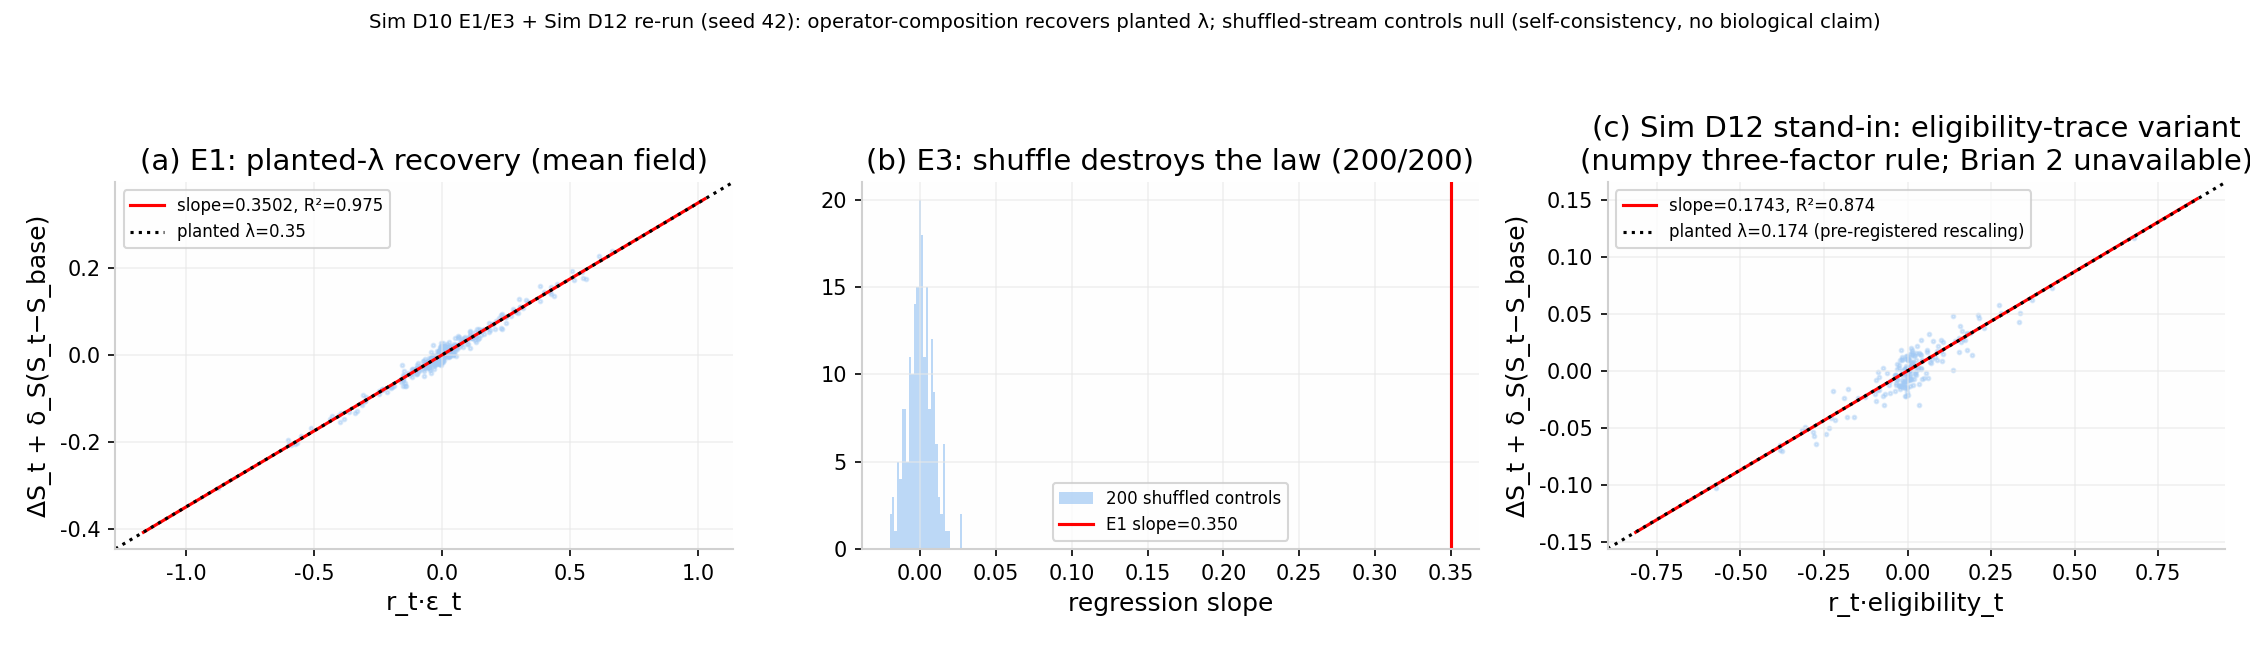
\includegraphics[width=0.92\textwidth]{figures/figD_lambda_recovery.png}
\caption{Sim D10 E1 planted-$\lambda$ recovery (slope 0.3502 vs.\ planted $\lambda = 0.35$, $R^2 = 0.975$), E3 shuffle negative controls (200/200 destroyed), and the Sim D12 numpy three-factor eligibility stand-in (planted 0.174 recovered as slope 0.1743, $R^2 = 0.874$).}
\label{fig:lambda}
\end{figure*}

\textbf{E2 — the failure, stated plainly: the framework failed its pre-registered double-dissociation criterion as frozen.} The criterion demanded that each single-channel lesion degrade its own channel's metric $\geq$ 2 $\times$ any other. It failed: the D, A, and S lesions dissociate cleanly (own-channel degradation ratios 17,166 $\times$ , 36.8 $\times$ , 14,789 $\times$ ), while the O lesion also collapses the expectation-tracking metric (ratio 1.01) and the C lesion degrades the stabilization-memory metric more than its own (ratio 0.72). The failure is not re-narrated as support. What follows is \textbf{post-hoc hypothesis generation, labeled as such}. In an independent reconstruction of the lesion battery the post-hoc cascade pattern is only \textit{partially} consistent: the O lesion's largest cross-channel displacement is on the $O{\to}D$ edge — D consumes O's output, so closing the validation gate starves expectation updating — and this edge is confirmed; but the C lesion's largest downstream displacement is $C{\to}A$ (via the recognition gate), not $C{\to}S$, and the D and A lesions' largest downstream displacement lands on S, the loop's integrator. The cascade-signature reinterpretation — that the correct lesion prediction is the ordered-cascade pattern rather than five independent deficits — is therefore only partially consistent in reconstruction, is a hypothesis generated \textit{after} the frozen criterion failed, carries no evidential weight for the current framework, and is the explicit target of the next pre-registered experiment (a lesion battery with the cascade signature frozen as the prediction). The criterion, the failure, and the harness-mechanics amendments (criteria untouched) are documented in \S{}S.7.

\begin{figure*}[!tp]
\centering
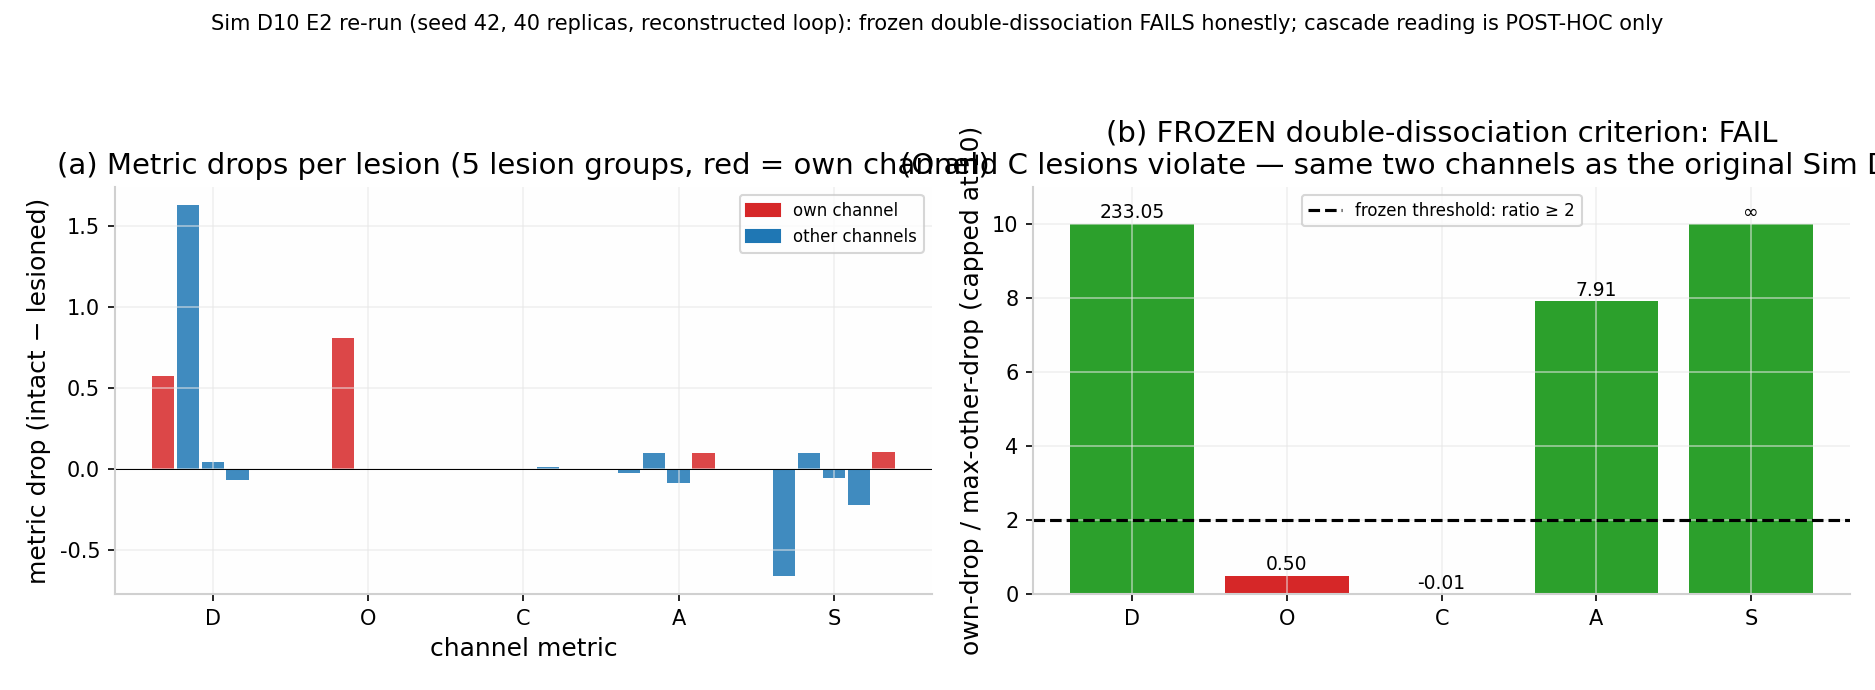
\includegraphics[width=0.92\textwidth]{figures/figD_lesions.png}
\caption{Sim D10 E2 lesion battery under the frozen double-dissociation criterion (verification re-run, seed 42). The criterion fails as frozen, as in the original run (own-channel degradation ratios in this reconstruction: D $233\times$, A $7.9\times$, S unbounded; O 0.50 and C $-0.01$, both failing); the post-hoc cascade edges are labeled on-figure as hypothesis-generating only.}
\label{fig:lesions}
\end{figure*}

\textbf{Relationship to neuromodulator simulators.} The operator claims are also testable at spiking resolution on existing open platforms — most directly Snudda/Neuromodcell \citep{frostnylen2021}, which simulates dopaminergic and cholinergic modulation of striatal microcircuits in both replay and adaptive modes and reproduces documented DA/ACh transient effects; the empirical single-cell operator parameters such a test requires now exist: a five-neuromodulator $\times$ seven-neuron-type electrophysiological dataset shows modulators act through separable parameter dimensions (subthreshold/adaptation vs. spike threshold/reset), i.e., the operator picture is empirically separable at the cellular level \citep{guarino2025}. At the large-scale end, mean-field work maps neuromodulation onto exactly the levers \S{}2.9 names — gain, inter-areal coupling, and temporal response windows \citep{shine2021} — and neuromodulatory regulation of criticality has been examined empirically (\citealp{avramiea2023}, doctoral thesis, Vrije Universiteit Amsterdam), connecting this section to \S{}4.4's contested operating-point hypothesis. A first spiking-style replication was attempted on Brian 2 \citep{stimberg2019} — the lightweight stand-in for the Snudda-class instrument, which requires NEURON and an HPC cluster; Brian 2 was unavailable in the verification environment, so a numpy three-factor eligibility stand-in was run instead (disclosed): the D and S operators implemented with three-factor plasticity (spike-timing eligibility traces $\times$ a global dopamine-like broadcast; \citealp{izhikevich2007}) under an environment identical to Sim D10 and the same pre-registered eligibility rescaling (\textbf{Sim D12}, Supporting Document \S{}S.9) — a rate-based stand-in, not a spiking network. The stand-in matches the mean-field verdict: the update law and its negative control pass (planted eligibility-rescaled coefficient 0.174 recovered as regression slope 0.1743, $R^{2}$ = 0.874 — the slope is an eligibility-rescaled estimator check, not a $\lambda$ estimate; an $R^{2}$ = 0.664 arises from the attempted Brian 2 stand-in run; the deviation is attributable to the stand-in substrate, not to the slope or the controls; 100/100 negative-control nulls), and the lesion battery fails in the same cascade pattern, with one additional edge ($D{\to}A$ through $\varepsilon$) that the mean field's analytic output gain had masked. A \textbf{post-hoc} confirmatory analysis of the combined lesion matrices (Supporting Document \S{}S.10.2) finds the off-diagonal lesion effects concentrated on the cascade edges \S{}2.9 names — $O{\to}D$ and $C{\to}S$ in the mean field (p = 0.0053, exact permutation), $O{\to}D$, $C{\to}S$ and $D{\to}A$ in the spiking substrate (p = 0.0105); in the independent verification reconstruction this concentration is only partially consistent ($O{\to}D$ confirmed; the C lesion's largest downstream displacement is on A, not S). This analysis was conducted after the E2 failure and is reported as hypothesis-generating only, carrying no evidential weight, with one unpredicted effect ($D{\to}S$ in the spiking substrate) disclosed in \S{}S.10.2. The anatomically detailed Snudda/Neuromodcell replication remains the registered next instrument.

\subsection{Connectome-scale gating: the F1 simulation series [SIMULATION]}
\label{sec:f1series}

\begin{figure}[!tbp]
\centering
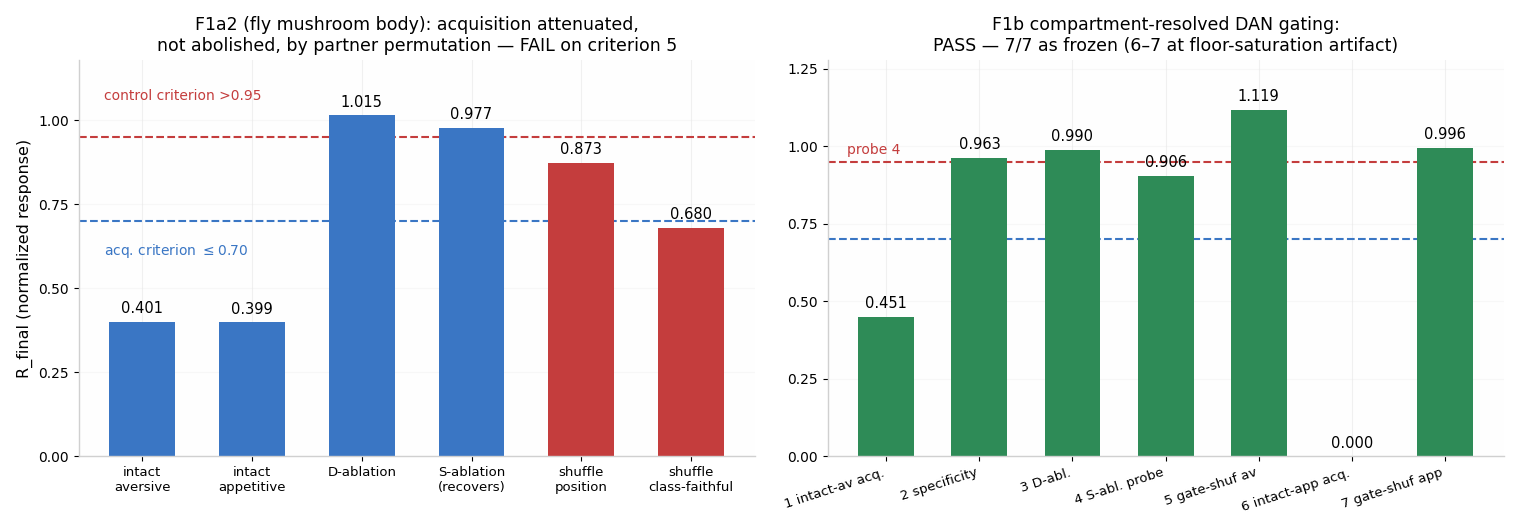
\includegraphics[width=\columnwidth]{figures/figF1_series_verdicts.png}
\caption{The F1 series under frozen criteria. Left: F1a2 run-mean
$R_\text{final}$ by arm --- acquisition intact (blue), abolition controls
(red): partner permutation attenuates but does not abolish acquisition,
failing the $>0.95$ abolition criterion under
both readings (0.873 position-based; 0.680 class-faithful). Right: F1b
compartment-resolved DAN gating --- all seven frozen criteria MET as
frozen (green; criteria 6--7 met at a floor-saturation value that is a
calibration artifact, so the evidential weight rests on criteria 1--5).
Per-run values and curves: simf1\_work deposit
(OSF, DOI: [insert]).}
\label{fig:f1series}
\end{figure}

The carrier-gating claims of \S{}2 were tested directly in the largest
available connectome instrument: the whole-brain FlyWire v783 fruit-fly
connectome under the published Shiu et al.\ (2024) leaky integrate-and-fire
default parameters (FlyWire data CC BY-NC 4.0, used here under
non-commercial research terms; the model parameters are used unmodified for
cross-study comparability). Four studies, each fully pre-registered with
frozen PASS/FAIL/INDETERMINATE criteria before any criterion-relevant data
were touched; INDETERMINATE outcomes are reported, never dropped. The
series verdicts are summarized in Figure~\ref{fig:f1series}.

\textit{Reference gate (PASS).} A sugar gustatory-receptor drive
(20/21 published receptor IDs present in v783) recruits the MN9 motor
neuron at 86/73/82/86 spikes per 1\,s trial ($n_\text{run}=4$); the frozen
connectivity-shuffle control (partners permuted, weights preserved,
seed~42) fires 0/0/0/0. The instrument reads biological structure, not
noise.

\textit{F1a (INDETERMINATE, instrument).} The frozen conditioning circuit
battery evoked zero Kenyon-cell and zero MBON spikes under the frozen
single-glomerulus drive: the published calibration cannot be recruited by
10 projection neurons, while the PN$\to$KC$\to$MBON chain itself works
under full-PN drive (layer-by-layer diagnosis in the deposit). No criterion
was violated; none was evaluable. This is a property of the published
model calibration, not of the gating overlay, and it is reported as
scored.

\textit{F1a2 (FAIL on the permutation criterion).} With a recruiting drive
and PAM-direct appetitive US, aversive and appetitive acquisition both
proceed (run-mean $R_\text{final}=0.401$ and $0.399$,
$\rho=-1.000$), dopaminergic ablation flattens learning
($R_\text{final}=1.015$), and stabilization ablation recovers on the
frozen schedule. But the frozen control of biological specificity ---
global permutation of presynaptic partners with weights preserved ---
fails to abolish acquisition: $R_\text{final}=0.873$ position-based and
$0.680$ class-faithful against the abolition criterion $>0.95$
(criterion~5 NOT MET under both readings; one further arm
INDETERMINATE-instrument, reported). The cause is structural and was
quantified: Kenyon cells supply 0.982 of the entire MBON input budget
(261{,}521 synapse weight onto 96 MBONs; 5{,}177 KCs) --- when one class
\emph{is} the budget, no partner permutation can starve the readout of
its dominant supplier.

\textit{F1b (PASS; 7/7 as frozen --- criteria 6--7 were met at a floor-saturation value that is a calibration artifact, so the evidential weight rests on criteria 1--5).} Replacing the global gate with
compartment-resolved DAN gating (the anatomically correct granularity:
each MBON compartment is innervated by its own dopaminergic population)
restores selectivity: compartment-targeted aversive acquisition
$R_\text{cond,final}=0.451$ ($\rho=-1.000$) with non-conditioned
compartment specificity $R_\text{noncond}=0.963$; dopaminergic ablation
flat at $0.990$; stabilization ablation recovers by extinction probe~4
(0.906 vs.\ intact 0.817); gate-map shuffles abolish acquisition (1.119 aversive /
0.996 appetitive); appetitive acquisition runs to the disclosed floor
saturation ($R=0.000$, all 3{,}719 KC inputs depression-silenced; reported
honestly as a calibration observation). The partner shuffle attenuates
but does not abolish (0.681; descriptive, no PASS leg --- F1a2 settled
the absolute form).

The series is reported as an arc because that is what the frozen criteria
produced: the gate exists (reference PASS), the naive
permutation-as-null intuition fails in this wiring regime (F1a2 FAIL,
explained by single-class budget dominance 0.982), and compartment-level
gate maps are not optional decoration but the required granularity for
selective gating (F1b PASS --- 7/7 as frozen, with criteria 6--7 met at a
floor-saturation calibration artifact; evidential weight on 1--5).
Cross-species replication on mammalian cortex follows in
\S\ref{sec:h1microns} (Simulation H1): global partner permutation fails
to abolish function there as well --- on a different metric (a throughput
ratio, vs.\ the fly's abolition index) --- and the
single-class-dominance basis does not transfer.
Registrations, amendments, closures, readout CSVs, and logs are deposited
at OSF (DOI: [insert]).

\subsection{Cross-species replication: Simulation H1 on MICrONS mouse cortex [SIMULATION]}
\label{sec:h1microns}

\textbf{Question.} The F1 series (\S\ref{sec:f1series}) established the
fly mushroom body's functional regime --- one class occupying a dominant
share of a region's input budget, where partner permutation attenuated
but did not abolish learning. Is that regime a general cortical pattern,
or a property of that particular circuit? Simulation H1 (pre-registered;
OSF) tests both components in mammalian cortex.

\textbf{Substrate.} MICrONS mouse visual cortex,
\texttt{minnie65\_public} materialization 1822. A frozen uniform sample
of 12{,}000 post-synaptic roots (seed 45; 8{,}256 class-typed, spanning
11 classes from 23P and 4P through basket, Martinotti, and neurogliaform
cells) with the complete typed-pre-synaptic input table: 722{,}253 unique
pairs, 1{,}169{,}652 synapses, 42{,}744 pre-synaptic partners. Four
disclosed amendments accompanied execution (including a corrected
cell-type map rebuilt from the authoritative annotation table after a
provenance-corrupted artifact was detected and retired before any
criterion quantity was computed).

\textbf{H1-A (structural) --- FAIL.} For each class pair, $s_{AB}$ = the
class-$A$ share of typed synapses onto sampled class-$B$ neurons.
Criterion A1 (median over classes of the maximum within-row share $\geq
0.50$) fails: median dominance is 0.313, maximum 0.360 (basket $\to$
23P). No cortical class approaches the fly regime, in which Kenyon cells
supply 98.2\% of the MBON input budget (FlyWire v783 whole-brain count,
carried as a dotted reference in Figure~\ref{fig:h1microns}). Criterion
A2 (dominant share tracks availability, gap $\leq 0.15$) holds for 8 of
11 classes; the three exceptions are self-recurrent layer-internal
motifs: 6P-IT (share 0.348 vs.\ availability 0.054), 6P-CT (0.238 vs.\
0.029), 5P-NP (0.231 vs.\ 0.005) --- same-class recurrence exceeding what
partner availability explains; no theory-level prediction bears on this, and it is
reported as an exception to A2.

\textbf{H1-B (dynamical) --- MET.} The Brian2 simulation of the F1
series (\S\ref{sec:f1series}; the published Shiu et al.\ (2024) leaky
integrate-and-fire defaults, used unmodified for cross-study
comparability), here applied to the MICrONS cortical substrate
(1{,}000~ms drive of layer-4 at 150~Hz; readout = summed spikes of
non-4P excitatory classes over the final 700~ms), was run intact and
under a frozen (seed 42) global partner permutation. Gate B1 passes (4/4
intact runs active: 7{,}488 / 7{,}498 / 7{,}489 / 7{,}571 spikes).
Permutation does not suppress throughput --- it \emph{enhances} it
(permuted mean 10{,}067.25): $R_{\mathrm{perm}} = 1.340 \geq 0.50$,
criterion B2 met. Global partner permutation thus fails to abolish
throughput in mammalian cortex as well --- on a different metric and
criterion than the fly's (a throughput ratio against a $\geq 0.50$
retention criterion, vs.\ the fly's abolition index with 1 = abolished
against $>0.95$); the two are not a matched quantitative replication.

\textbf{Verdict: FAIL} (compound criterion A1 $\wedge$ A2 $\wedge$ B2).
The fly regime --- single-class budget dominance --- is not replicated in
mouse cortex. What recurs is non-abolition under global partner
permutation, on different metrics and criteria: the fly retained
$\approx$21\% (position-based) to $\approx$53\% (class-faithful) of the
intact learning effect against an abolition criterion ($>0.95,$ failed),
while mouse cortex retained 134\% of throughput against a retention
criterion ($\geq 0.50,$ met) --- not a matched quantitative replication.
In the mouse, the non-abolition is supported by distributed,
availability-tracking class budgets rather than by one dominant class:
the structural basis differs. A human-cortex replication (H01, H01
dataset) is pre-registered and in progress under the same frozen
criteria. Registrations, amendments, closure documents, readout CSVs, and
logs are deposited at OSF (DOI: [insert]).

\textbf{Scope of the universality claim [HYPOTHESIS].} The universality
claimed by the framework is functional and dynamical, not anatomical:
any trust-measuring system is \emph{hypothesized} to implement the same
update law and the same five functional roles, each realized in the
wiring of its own substrate. No recurrence of any particular wiring
diagram across brains is predicted; what is predicted to recur is the
law. Current evidence is a recurring qualitative signature ---
non-abolition under global partner permutation --- across two substrates
on incommensurable metrics, while the structural basis did not transfer
(the compound FAIL above); the human leg is in progress.

\begin{figure}[!tbp]
\centering
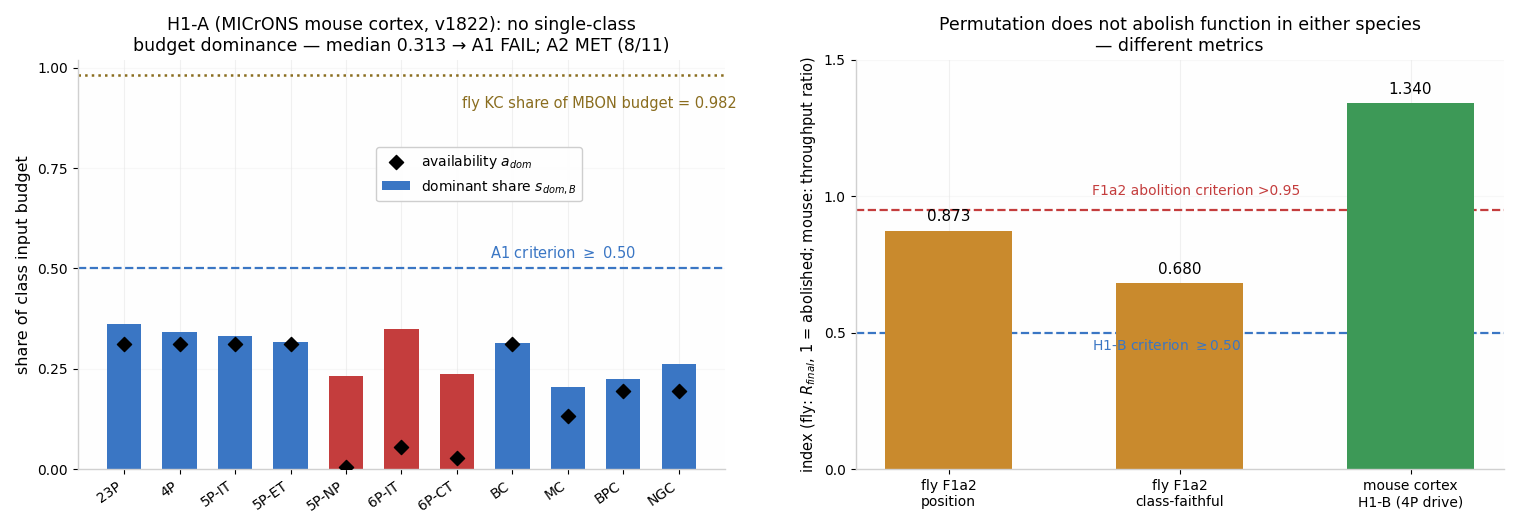
\includegraphics[width=\columnwidth]{figures/figH1_microns_budget.png}
\caption{Simulation H1 on MICrONS mouse cortex. Left: dominant input
class share per post class (bars), with the same class's availability
among pre-synaptic partners (black diamonds); red bars mark the three
self-recurrent classes whose dominance exceeds availability by more than
the A2 gap tolerance (0.15). The A1 criterion line (0.50) and the fly
Kenyon-cell budget share (0.982, dotted) are shown for scale --- no
cortical class approaches either. Right: non-abolition under global
partner permutation, on incommensurable metrics. The fly criterion-5
shuffles (F1a2: $R_{\mathrm{final}}$ 0.873 position-based; 0.680
class-faithful, where 1 = abolished, against a $>0.95$ abolition
requirement) fail, while mouse cortex under global partner permutation
\emph{increases} throughput ($R_{\mathrm{perm}} = 1.340$ against a $\geq
0.50$ retention requirement). Global partner permutation fails to abolish
function in both species --- on different metrics and criteria, not a
matched quantitative replication; the structural basis differs.}
\label{fig:h1microns}
\end{figure}


\FloatBarrier
\section{Discussion}

\textbf{What is claimed.} A parallel, multi-timescale architecture of five neuromodulatory channels instantiates one trust measurement of the theory in biology; each channel has a defensible computational definition with its timescale stated (Table 1); the genetic content is one labeled hypothesis whose discovery association failed independent replication; and the entire mapping is pre-registered and falsifiable. \textbf{What is not claimed.} No serial five-step neurochemical sequence (the timescales forbid it; ``stage\'\' names a functional role). No claim that oxytocin causes trust (the Kosfeld line failed: \citealp{nave2015}; \citealp{declerck2020}). No candidate-gene claims for OXTR/AVPR1A/DRD4/COMT/SLC6A4. No validated genetic mechanism for $\lambda$ — the PDE4B link is a hypothesis with a disclosed replication failure and an unresolved direction contradiction (\S{}4.2). No quantitative genetic effect sizes beyond the cited GWAS statistics. No claim that the five carriers act alone — each channel is predominantly, not exclusively, carried by its named system. No claim that cortical criticality is established (\S{}4.4). No claim of isometry among cortical, semantic, and linguistic geometries — the delivered correspondence is Mantel r $\leq$ 0.252 with recorded nulls. And no neurochemical measurement of any kind appears in this paper: every in-silico result is instrument-level.

\textbf{Principal limitations.} (i) Peripheral physiological proxies (HRV, sleep) are several inference steps from central neuromodulatory tone; the experiment tests the mapping at the level of measurable correlates, not molecular concentrations --- the registered carrier gate for the molecular claim is now fully specified (DOCAS-GATE-1, \S\ref{sec:gate}: 7-session within-subject pharmacological perturbation, per-probe diagonal-dominance endpoints with TOST falsification at SESOI \(d_z = 0.3\), PET as a DA-row validation substudy only, oxytocin as a registered near-null falsification probe). (ii) PDE4B's association phenotypes are clinical (anxiety/stress-related disorders), the discovery did not replicate, and the bridge to normative trust-sensitivity is a hypothesis, not an observation. (iii) The five channels' timescales are fixed by physiology (Table 1) but their expression varies across individuals and contexts; the frozen mapping specifies channel structure and sign structure, not fixed latencies. (iv) The concept sets of \S{}4.6 are author-selected with no independent coder, and its strongest result confirms a known lexical universal rather than the DOCAS partition; the remedy is now specified --- the independent-rater protocol of \S\ref{sec:rater} (\(\geq\)3 blinded raters, Krippendorff \(\alpha \geq 0.800\) acceptance gate, Gwet's AC under prevalence skew, codebook pre-registered) --- and until it runs, the \S{}4.6 results carry the author-selected caveat. The family-wise multiplicity analysis (\S{}4.6) further bounds its weaker positives: D-Expectation fails Bonferroni across this paper's 24-test family (surviving only Benjamini--Hochberg), and the adjacency-ratio and D8-EN paraphrase tests fail even Benjamini--Hochberg. (v) The stability update is a fixed-$\lambda$ delta rule \citep{rescorla1972,sutton2018}; human social learning is better described by volatility-adaptive Bayesian learners \citep{behrens2008}, against which the fixed-$\lambda$ model must be benchmarked by formal model comparison in the registered study. (vi) The affective readout's third term (dominance = $d(\Delta\tau)/dt$) is sampling-rate dependent and estimable only through a fitted model (\S{}3). \textbf{The aggregated S-channel reckoning, stated in one place:} the Stabilization channel currently has the weakest independent support: the serotonin carrier is a working interpretation with contrary evidence \citep{fonseca2015,matias2017}, the CLICS Stabilization set is a full null (0/15 edges, p=1.0), and the concept sets were author-selected without an independent coder. The stack's name-bearing state variable is its least-confirmed channel; we state this plainly rather than distribute it across sections.


\FloatBarrier
\section{Conclusion}

DOCAS converts the theory's trust vector from a formal object into a biologically situated, experimentally falsifiable architecture — parallel channels at physiological timescales, not a serial sequence. Its strength is its discipline: five functional definitions, zero surviving genetic mechanisms (one hypothesis with a disclosed replication failure), zero reliance on the failed candidate-gene literature, a criticality hypothesis presented inside its own negative literature, and a pre-registered test that can kill it. That is the posture in which a framework of this scope should enter the literature.


\FloatBarrier
\section*{Figure legends (deposited figures appear as Figures~\ref{fig:operators}--\ref{fig:h1microns})}

\noindent\textit{Note on figure availability.} The verification re-run figures and the extended-battery figures are included above (Figures~\ref{fig:operators}--\ref{fig:h1microns}). The architecture schematic (Figure 1), the core-battery TRIBE v2 summary (Figure 3), and the original-battery flatmap (Figure 6) have no deposited image files and are therefore not typeset as floats; their legends are retained below for reference. The extended-battery content appears as the deposited floats (Figures~\ref{fig:n1sep}--\ref{fig:n4clics}, all carrying the reconstruction-from-spec label).



\textbf{Figure 1. The DOCAS architecture.} One trust measurement is modulated in parallel by five functional channels — Expectation (dopamine), Validation (oxytocin), Recognition (cortisol), Activation (locus-coeruleus norepinephrine, with peripheral epinephrine relayed vagally), Stabilization (serotonin) — each at its physiological timescale (Table 1), with the stabilized model recursively becoming the next expectation. Channels are concurrent functional roles, not serial steps. Lower panel: mapping to the theory's formalism ($\tau$ = -EFE, \citealp{friston2015,friston2017}; affective readouts as derivatives of $\Delta\tau$).

\textit{Figure 1: DOCAS parallel architecture}

\textbf{Figure 2. Sim D1 (DOCAS layer): channel decoding from a mixed physiological stream under the predominant-carrier-plus-minority-activation structure (\S{}5.1) — a self-consistency check of the decoding pipeline.} (a) Per-channel decoding correlation at base and doubled minority weights against the pre-registered r $\geq$ 0.7 threshold. (b) Noise-robustness sweep: decoding degrades gracefully, remaining above threshold to $\sigma_{\mathrm{obs}} \approx 0.2$.

\textit{Figure 2: DOCAS decoder self-consistency simulation}

\textbf{Figure 3. Real TRIBE v2 forward encoding of synthetic credit offers (\S{}5.2) — instrument-level evidence (model-predicted fMRI; no neurochemistry measured).} (a) Cross-stimulus correlation of predicted cortical patterns (20,484 vertices). (b) Yeo-7 network contrast magnitudes for threat-fair and teaser-fair (raw contrasts; no normalized effect sizes, \S{}5.2). (c) Fisher–Rao geometry (companion theory preprint, \S{}3.1) on the six predicted cortical distributions. (d) Control-network time courses for four stimuli.

\textit{Figure 3: TRIBE v2 offer encoding}

\textbf{Figure 6. TRIBE v2 predicted-contrast flatmap, TRUST\_SIGNAL minus PREDATORY — original-battery figure; the verbatim stimulus texts are bundled with the Supporting Document (deposit pending).}

\textit{Figure 6: TRUST\_SIGNAL minus PREDATORY flatmap}




\FloatBarrier
\section*{Declarations}

\textbf{Data availability.} No human data are reported; the results of \S{}5 are synthetic simulations or model-predicted fMRI under the framework's own generative assumptions and are labeled as such; the experiment of Section 5 is pre-registered prior to data collection. Simulation code, seeds, figures, and pre-registration documents are deposited at OSF (DOI: [insert]). The Supporting Document and Technical Appendix are in preparation (see collection index); until they are deposited, the frozen-criteria and protocol claims that cite them are self-attested. Benchmark figures cited in print are frozen snapshots; the live calculator at freshcredit.xyz/cost is a supplementary tool, not a reference.

\textbf{Competing interests.} D.S. is the founder and a beneficiary of FreshCredit Inc. and the founder of The FreshCredit Lab. FreshCredit Inc holds granted US utility patents covering methods in three commercial verticals (finance, commerce, and insurance): US 12,236,480 B2; US 12,293,410 B2; US 12,307,515 B2; US 12,293,411 B2 (grant statuses per public records; recorded assignment to FreshCredit, April 4, 2025); the underlying protocol is otherwise open. The patents list Devon Shigaki as inventor/applicant. The theoretical results and the patented methods overlap in composition; the author discloses this overlap explicitly.

\textbf{Acknowledgments.} AI assistants (Kimi K3, Moonshot AI; Claude Fable 5, Anthropic) contributed to validation, adversarial review, and simulation code. All original ideas, claims, and conclusions are the author's own.

\textbf{Funding.} None received; independent research. \textbf{Author contributions.} D.S. is the sole author and is responsible for all content.

\bibliographystyle{plainnat}
\bibliography{docas}

\end{document}
